% Gelfand seminar notes, 1975-76: source pages P000603-P000658.
% English translation (AI-made, checked against the scans), cut page by page from the cumulative working reader A4-reader-chapters01-34-complete-first1527-separated-diplomatic-r5.
% \SourcePage{GELFAND-Pnnnnnn}{label} starts a scanned page; the second argument is the number written
% on the page, if any. Editorial notes give the page, a label and the transcriber's remark; \Unclear
% marks a doubtful reading.
\SourcePage{GELFAND-P000603}{unlabelled}
\underline{\underline{15.9.75.}}\qquad\underline{Gelfand Sem.}

There will be a series of lectures by \uwave{Polyakov} on physics.

\underline{\underline{Kirillov.}}\qquad\uwave{Thm. J. Vey} on deformation of the Poisson bracket.
\Unclear{GELFAND-P000603}{vey-initial}{The initial reads “J.”.}
\end{GelfandAdjacentEvidence}
\begin{GelfandAdjacentEvidence}{GELFAND-P000603}{2}


\((M,\omega)\) — a sympl. manifold, \([u,v]\) — the Poisson bracket.
There are essentially no other Lie alg. structures (Kirillov et al.). But if diff. oper. of order \(\infty\) are allowed, the structure can be deformed.

\underline{Thm.:} \(\exists\) a formal deformation of the Poisson bracket, inequivalent to it.
\[
[u,v]_t=\sum_{k=0}^{\infty}t^k[u,v]^{(k)}
\]
[stroke from \([u,v]^{(k)}\):] oper. of order \((2k+1)\) in \(u\) and \(v\).

nontriviality: a change of coordinates does not reduce it to the original Poisson bracket.
\[
[u,v]^{(k)}=\frac{1}{(2k+1)!}\left(
\frac{\partial^{2k+1}u}{\partial p^{2k+1}}
\frac{\partial^{2k+1}v}{\partial q^{2k+1}}-
\frac{\partial^{2k+1}u}{\partial q^{2k+1}}\cdot
\frac{\partial^{2k+1}v}{\partial p^{2k+1}}\right)+\ldots
\]
\hfill lower terms\par
On the plane (or torus) there are no lower terms.
\Unclear{GELFAND-P000603}{lower-terms-abbreviation}{The abbreviation in both places tentatively reads “мл.” (lower).}
\end{GelfandAdjacentEvidence}


Defined globally on \(M\) provided that \(H^3(M,R)=0\).
\[
?\qquad pq-qp=t
\]


\Needspace{7\baselineskip}
\begin{GelfandAdjacentEvidence}{GELFAND-P000604}{1}
\SourcePage{GELFAND-P000604}{unlabelled}
\underline{\underline{Polyakov.}} (\underline{Alexander Markovich}).

\underline{Elementary particle physics.}

\underline{\(\gamma\) — photon.} — a separate group

\underline{Leptons}
\[
\begin{array}{@{}l@{}}
\begin{array}{@{}ll@{}}
e^- & m=0{,}5\\
\mu^- & m=105
\end{array}\\[-.1ex]
\left.\begin{array}{@{}ll@{}}
\nu_e & m=0\\
\nu_\mu & m=0
\end{array}\right\}\text{ neutrinos}
\end{array}
\]
\par\noindent\rule{.31\linewidth}{.45pt}\par

\underline{Hadrons.}
\[
\begin{array}{ll}
p & m=940\\
n & \text{— \(\Vert\) —}\\
\pi & m=140
\end{array}
\]
etc.
\par\noindent\rule{.31\linewidth}{.45pt}\par
\Unclear{GELFAND-P000604}{pion-mark}{The top stroke of \(\pi\) is separate from the lower strokes.}
\end{GelfandAdjacentEvidence}
\begin{GelfandAdjacentEvidence}{GELFAND-P000604}{2}


\underline{Interactions:}\qquad
\dashuline{Intensity in units} \(x=\dfrac{E_{\text{int}}}{m}\)
\[
\begin{array}{lll}
\mathrm{Gr} & (\text{gravit.}) & x\sim10^{-38}\\
\mathrm W & (\text{weak}) & x\sim10^{-5}\\
\mathrm{EM} & (\text{electromagn.}) & x\sim10^{-2}\\
\mathrm S & (\text{strong}) & x\sim1
\end{array}
\]
The weaker the interact., the more accommodating it is (it violates fewer conservation laws).

They are distinguished only by symmetry (the strong from the weak, since both are [crossed out] short-range).
\Incomplete{GELFAND-P000604}{cancel-after-oba}{The word after “both” is heavily crossed out.}
\end{GelfandAdjacentEvidence}
\begin{GelfandAdjacentEvidence}{GELFAND-P000604}{3}


\underline{Leptons} — all interact. except the strong.

\underline{Hadrons} — all 4 interactions.

\uwave{Quantum electrodynamics} describes the electromagn. interact. of leptons. (the others are weaker and are ignored for now).

A particle is described by its own field. One must specify the action:
\[
S=S[e(x),\mu(x),\ldots]
\]
Invariance: rot., transl., Lorentz transf..

\dashuline{Exper. fact}: under rot. the electron transf. according to the spinor representation
\[
\begin{pmatrix}e'_1\\e'_2\end{pmatrix}
=\exp\left(\frac i2(\bar\sigma\,\bar\Theta)\right)
\begin{pmatrix}e_1\\e_2\end{pmatrix}
\]
\hfill(\(e_j\in\mathbb C\) — components of the spinor)\par

\(\bar\sigma\) [crossed out] — Pauli matrices (a set of 3 such matrices); \(\bar\Theta\in\mathbb R^3\);
\Unclear{GELFAND-P000604}{cancel-after-sigma}{The entry after \(\bar\sigma\) is heavily crossed out.}
\end{GelfandAdjacentEvidence}


\(|\bar\Theta|\) — angle of rot., dir. of \(\Theta\) — dir. of the axis of rotation.


\Needspace{7\baselineskip}
\begin{GelfandAdjacentEvidence}{GELFAND-P000605}{1}
\SourcePage{GELFAND-P000605}{unlabelled}
\[
\sigma_x=\begin{pmatrix}0&1\\1&0\end{pmatrix},\quad
\sigma_y=\begin{pmatrix}0&-i\\i&0\end{pmatrix},\quad
\sigma_z=\begin{pmatrix}1&0\\0&-1\end{pmatrix}.
\]
\Unclear{GELFAND-P000605}{matrix-upper-entry}{There is a short stroke before the upper right 1 in \(\sigma_x\). It may be a minus.}
\end{GelfandAdjacentEvidence}
\begin{GelfandAdjacentEvidence}{GELFAND-P000605}{2}

Calc. also the transf. under the action of the Lorentz group. 2 possibilities:
\Unclear{GELFAND-P000605}{initial-verb}{The initial abbreviation tentatively reads “Вычис.” (calc.).}
\end{GelfandAdjacentEvidence}
\begin{GelfandAdjacentEvidence}{GELFAND-P000605}{3}

\[
e'_L=\exp\left(\frac{\bar\sigma\bar\psi}{2}\right)e_L,
\]
where \(\bar\psi\) — a vector collinear with the velocity vect.:
\[
v=\operatorname{th}|\bar\psi|,\qquad
\frac{\vec v}{|\bar v|}=\frac{\bar\psi}{|\bar\psi|}
\qquad(\bar\psi\text{ — also a 3-vector})
\]
[below the line] “rapidity”
\[
e'_R=\exp\left(-\frac{\bar\sigma\bar\psi}{2}\right)e_R
\]
\rule{.21\linewidth}{.4pt}\par
\underline{Explan.} (G.) [crossed out]. \(SO(3)\longrightarrow\)
[crossed out]. \(SU(2)\).
\Incomplete{GELFAND-P000605}{cancel-before-so}{An entry before \(SO(3)\) is crossed out.}
\end{GelfandAdjacentEvidence}
\begin{GelfandAdjacentEvidence}{GELFAND-P000605}{4}

\Incomplete{GELFAND-P000605}{cancel-before-su}{An entry before \(SU(2)\) is crossed out.}
\end{GelfandAdjacentEvidence}
\begin{GelfandAdjacentEvidence}{GELFAND-P000605}{5}

\Unclear{GELFAND-P000605}{so-su-direction}{The handwritten arrow points from \(SO(3)\) to \(SU(2)\).}
\end{GelfandAdjacentEvidence}
\begin{GelfandAdjacentEvidence}{GELFAND-P000605}{6}

\[
\bar\Theta\text{ — rot. in }\mathbb R^3\Longrightarrow\text{matr.}\in SU(2)
\]
(representation of \(SU(2)\))

This rep. extends to a rep. of the Lorentz group.

Lorentz transf. — the velocity vector \(\vec v\) (rotation is omitted)
(proper Lorentz transf.)

\uwave{Rapidity} \(\bar\psi\) — introduced in place of \(\bar v\)

\rule{.28\linewidth}{.4pt}\par
\underline{\underline{P.}}
\[
\left\{\begin{aligned}
t'&=t\operatorname{ch}\psi+z\operatorname{sh}\psi\\
z'&=z\operatorname{ch}\psi+t\operatorname{sh}\psi
\end{aligned}\right.
\]
\Unclear{GELFAND-P000605}{boost-z-overwrite}{In the first line \(z\) is written over an earlier mark.}
\end{GelfandAdjacentEvidence}
\begin{GelfandAdjacentEvidence}{GELFAND-P000605}{7}

[at right] — Lorentz transf. written in terms of \(\psi\).
(proper Lorentz transf. — with no added rot. or translation).

The electron is either \(e_L\) or \(e_R\).

But there is a symmetry \(\vec x\longrightarrow-\vec x\), \(\vec v\longrightarrow-\vec v\), they turn into each other.

If reflection is adjoined, the rep. is only obtained in combined form:
\[
\hat p\begin{pmatrix}e_L\\e_R\end{pmatrix}
=\begin{pmatrix}e_R\\e_L\end{pmatrix}.
\]
We need to introd. a \underline{bispinor}: \(\begin{pmatrix}e_L\\e_R\end{pmatrix}\).

Then the Lagrangian density:
\[
\begin{aligned}
\mathcal L'&=e_L^+(x)\left\{\frac{\partial}{\partial t}
-\left(\bar\sigma\frac{\partial}{\partial\bar x}\right)\right\}e_L(x)\\
&\quad+e_R^+(x)\left\{\frac{\partial}{\partial t}
+\left(\bar\sigma\frac{\partial}{\partial\bar x}\right)\right\}e_R(x)
\end{aligned}
\]
\((z^+=\bar z)\).

Action: \(S=\int\mathcal L\,dt\,d^3\bar x\).
\Unclear{GELFAND-P000605}{action-prime}{No prime is visible on \(\mathcal L\) in the action formula.}
\end{GelfandAdjacentEvidence}


Invariance is easy to check.

\underline{Masslessness}\qquad Lagr. eq.
\[
\left(\frac{\partial}{\partial t}-\bar\sigma\frac{\partial}{\partial\bar x}\right)e_L=0
\]
Take the Fourier transf.: \((E-\bar\sigma\bar p)e_L=0\) and hence \(E^2=p^2\).


\Needspace{7\baselineskip}
\begin{GelfandAdjacentEvidence}{GELFAND-P000606}{1}
\SourcePage{GELFAND-P000606}{unlabelled}
Hence \(E\) is arbitrarily small (for small \(p\)) \(\Rightarrow m=0\).

We must add a term with the mass. The inv. way is unique

\sout{\(e_L\)} [crossed out] \sout{\(me\)}
\Unclear{GELFAND-P000606}{canceled-mass-connector}{Under the crossing-out, the mark between \(e_L\) and \(me\) resembles a right-pointing arrow.}
\end{GelfandAdjacentEvidence}
\begin{GelfandAdjacentEvidence}{GELFAND-P000606}{2}

\begin{center}
\uwave{\(m(e_L^+e_R+e_R^+e_L)\)}.
\end{center}
Thus, the final form of the Lagrangian:
\[
\mathcal L=\mathcal L'+m(e_L^+e_R+e_R^+e_L).
\]
\underline{\underline{Equiv. form}}: let \(e=\begin{pmatrix}e_L\\e_R\end{pmatrix}\). (bispinor).
\[
\mathcal L=\bar e\left(i\gamma_\mu\frac{\partial}{\partial x_\mu}-m\right)e
\]
\[
\gamma_\mu\frac{\partial}{\partial x_\mu}
=\gamma_0\frac{\partial}{\partial t}-\bar\gamma\frac{\partial}{\partial\bar x},
\qquad \bar e=e^+\gamma_0
\]
\(\gamma_\mu\) — Dirac matr.,
\(\gamma_\mu\gamma_\nu+\gamma_\nu\gamma_\mu=2g_{\mu\nu}\),
\[
g_{\mu\nu}=\begin{pmatrix}
1&&&0\\
&-1&&\\
&&-1&\\
0&&&-1
\end{pmatrix}\text{ — Minkowski metr..}
\]
\(\gamma_\mu\) are written in terms of the matrices \(\sigma\)

(\underline{References}: Landau, Berestetskii, Lifshitz, Pitaevskii — Relativistic Quant. Theory, pt. 1).

\dashuline{Spectrum}: \(E=\sqrt{p^2+m^2}\).

(In the Dirac eq. \(\left(i\gamma_\mu\dfrac{\partial}{\partial x_\mu}-m\right)e=0\)
we pass to the Fourier transf. and obtain this res.)
\[
\rule{1.8em}{.4pt}\;\boldsymbol{\cdot}\;\rule{1.8em}{.4pt}
\]
\dashuline{Gauge group}\qquad \(e'\Rightarrow e^{i\beta}e\). \((\beta\in\mathbb R)\).
\Unclear{GELFAND-P000606}{gauge-arrow}{There are two horizontal strokes between \(e\prime\) and \(e^{i\beta}e\). The upper stroke has a point at the right.}
\end{GelfandAdjacentEvidence}
\begin{GelfandAdjacentEvidence}{GELFAND-P000606}{3}


\(\mathcal L\) is also invariant with resp. to this group\qquad \uwave{\(e'=(2{,}7\ldots)^{i\beta}e\)}

\dashuline{Hypothesis}: vary the phase differently at different points and require covar. with resp. to these transformations (extreme locality)
\[
\underline{e'=(2{,}7)^{i\beta(x)}e}
\]
\uwave{Invar. is now lost}:
\[
\bar e\left(i\gamma_\mu\left(\frac{\partial}{\partial x_\mu}+i\partial_\mu\beta\right)-m\right)e.
\]
\[
\mathcal L'=\bar e\biggl(i\gamma_\mu\frac{\partial}{\partial x_\mu}
+iA_\mu(x)\biggr)-m\biggr)e
\]
\Unclear{GELFAND-P000606}{a-term-contraction}{A closing parenthesis follows \(A_\mu(x)\), and another follows \(-m\). No factor \(\gamma_\mu\) is visible before \(iA_\mu(x)\).}
\end{GelfandAdjacentEvidence}



\Needspace{7\baselineskip}
\begin{GelfandAdjacentEvidence}{GELFAND-P000607}{1}
\SourcePage{GELFAND-P000607}{unlabelled}
(\(A_\mu(x)\) — a connection).
\[
\begin{gathered}
A'_\mu(x)=A_\mu-\partial_\mu\beta.\\
\nabla_\mu=\partial_\mu+iA_\mu.
\end{gathered}
\]
If we do this, general covariance will be restored.
\Unclear{GELFAND-P000607}{covariance-abbreviation}{The abbreviation before “covariance” reads “общ.” (general).}
\end{GelfandAdjacentEvidence}
\begin{GelfandAdjacentEvidence}{GELFAND-P000607}{2}


From \(\mathcal L'\) no eqs. arise for \(A_\mu\). We need the curvature
\[
F_{\mu\nu}=\partial_\mu A_\nu-\partial_\nu A_\mu
\]
This is a tensor, and in [crossed out] \(\mathcal L\) we introd. its square.
\Unclear{GELFAND-P000607}{cancel-before-l}{An entry before \(\mathcal L\) is crossed out.}
\end{GelfandAdjacentEvidence}
\begin{GelfandAdjacentEvidence}{GELFAND-P000607}{3}

\[
\mathcal L=\text{[crossed out]}\ \mathcal L'+\left(\frac1{4e^2}\right)F_{\mu\nu}^2
\]
\Unclear{GELFAND-P000607}{cancel-coefficient}{A sign before \(\mathcal L\prime\) on the right-hand side is crossed out.}
\end{GelfandAdjacentEvidence}
\begin{GelfandAdjacentEvidence}{GELFAND-P000607}{4}

(\(e\) — the electron charge)
\[
\rule{1.8em}{.4pt}\;\boldsymbol{\cdot}\;\rule{1.8em}{.4pt}
\]
\underline{Scattering.}\qquad \(S=S[\varphi(x)]\).
\[
B\qquad \varphi_{\mathrm{in}}(x)\longrightarrow\varphi_{\mathrm{out}}(x)
\]
\Unclear{GELFAND-P000607}{scattering-margin}{A separate mark to the left of the arrow resembles a B with a vertical stroke.}
\end{GelfandAdjacentEvidence}
\begin{GelfandAdjacentEvidence}{GELFAND-P000607}{5}

\[
\varphi_{\mathrm{in}}(x)=\lim_{t\to-\infty}\varphi(\bar x,t),\qquad
\varphi_{\mathrm{out}}(x)=\lim_{t\to+\infty}\varphi(\bar x,t).
\]
\[
\int_{\Phi_{\mathrm{in}}}^{\Phi_{\mathrm{out}}}D\varphi(x)\,e^{iS[\varphi]}
=M\text{ — transition amplitude}
\]
(functional integration, \(D\varphi\) — the natural measure, [below the line] (Lebesgue),
integral over all \(\Phi(x,t)\),
\(\Phi(x,+\infty)=\Phi_{\mathrm{out}}\),
\(\varphi(x,-\infty)=\varphi_{\mathrm{in}}\))

There are rules for calculation.

[crossed out] [inserted above the line and outlined] Without \(A_\mu\) — a Gaussian integral (Fresnel)
\Incomplete{GELFAND-P000607}{cancel-gaussian}{An entry before the insertion and the words “Gaussian integral” is heavily crossed out.}
\end{GelfandAdjacentEvidence}
\begin{GelfandAdjacentEvidence}{GELFAND-P000607}{6}


Then — perturbation theory (take \(A_\mu\) small); \(eA_\mu e\) — a cubic term

\rule{.22\linewidth}{.4pt}\par
\underline{G.}\qquad \(\int e^{i(x^2+\varepsilon x^3)}\,dx\) — your theory

Important:
\[
\int e^{-\sum a_{ik}x_ix_k+\varepsilon\sum x_i^3}\,dx
\]
\[
\int e^{ix^2(1+\varepsilon x^3)}=\sum c_k\int x^k e^{ix^2}\,dx
\]
\Unclear{GELFAND-P000607}{x-power-discrepancy}{The exponent reads \(ix^2(1+\varepsilon x^3)\).}
\end{GelfandAdjacentEvidence}
\begin{GelfandAdjacentEvidence}{GELFAND-P000607}{7}


For this we use Feynman diagrs.

[crossed out at left] \(\int\frac{\phantom{dx}}{(x^2+y^2+z^2+t\ldots)}\)
\Incomplete{GELFAND-P000607}{cancel-integral}{In the crossed-out entry the integral sign, fraction bar, and part of the denominator are legible.}
\end{GelfandAdjacentEvidence}
\begin{GelfandAdjacentEvidence}{GELFAND-P000607}{8}


E.g.
\[
\int\frac{dx\,dy\,dz\,dt}
{(x^2+y^2+z^2+t^2+m_1)(x^2+y^2+z^2+t^2+m_2)}
\]
\Unclear{GELFAND-P000607}{denominator-deletion}{A parenthesis is crossed out after the first \(t^2\). The exponent on \(y\) in the second factor is overwritten.}
\end{GelfandAdjacentEvidence}

(stolen by F. from Schwinger)
\[
\frac1{ab}=\int_0^1\frac{ds}{(sa+(1-s)b)^2}.\qquad
\frac1{abc}\text{ analogously.}
\]


\Needspace{7\baselineskip}
\begin{GelfandAdjacentEvidence}{GELFAND-P000608}{1}
\SourcePage{GELFAND-P000608}{unlabelled}
\underline{P.} one can also do \(\dfrac1{a^\lambda b^\mu c^\gamma}\)
\Unclear{GELFAND-P000608}{triple-exponent}{The exponent on \(a\) is overwritten and tentatively reads \(\lambda\).}
\end{GelfandAdjacentEvidence}
\begin{GelfandAdjacentEvidence}{GELFAND-P000608}{2}

\[
\frac1{a^\lambda b^\mu}
=\int_0^1\frac{s^{\lambda-1}(1-s)^{\mu-1}}{(sa+(1-s)b)^{\lambda+\mu}}\,ds
\]
\[
\frac1{\prod a_i^{\lambda_i}}
=\int_{s_i\geq0.}\frac{\prod ds_i\,\delta(\sum s_i-1)\,s_i^{\lambda_i-1}}
{(\sum s_i a_i)^{\sum\lambda_j}}
\]
\Unclear{GELFAND-P000608}{parameter-normalization}{Both formulas are written without a separate normalization factor.}
\end{GelfandAdjacentEvidence}
\begin{GelfandAdjacentEvidence}{GELFAND-P000608}{3}

\[
\rule{1.8em}{.4pt}\;\boldsymbol{\cdot}\;\rule{1.8em}{.4pt}
\]
We calculate by \dashuline{perturbation theory}:

\(x,\ x'\)

\uwave{Amplitude of trans. from \(x\) to \(x'\)}: \(K(x,x')\) according to Maxwell
\[
\left(i\gamma_\mu\frac{\partial}{\partial x_\mu}-m\right)K(x,x')=\delta(x-x').
\]
\Unclear{GELFAND-P000608}{kernel-gamma-writing}{The \(\gamma\) is heavily inked and may be overwritten.}
\end{GelfandAdjacentEvidence}
\begin{GelfandAdjacentEvidence}{GELFAND-P000608}{4}

\SourceFigure{GELFAND-P000608}{photon-exchange}{%
\par\smallskip
\begingroup\color{black}\GelfandFitDiagram{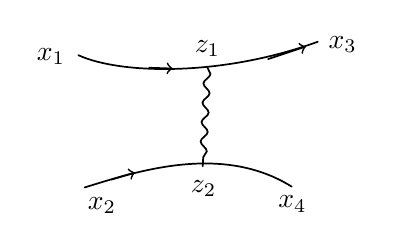
\begin{tikzpicture}[x=1cm,y=1cm,line width=.62pt,line cap=round]
\draw (0,1.90) .. controls (.52,1.66) and (1.8,1.62) .. (3.04,2.07);
\draw[->] (.90,1.74)--(1.20,1.73);
\draw[->] (2.41,1.85)--(2.89,2.01);
\draw (.08,.22) .. controls (.76,.43) and (1.83,.78) .. (2.71,.23);
\draw[->] (.42,.32)--(.72,.41);
\draw[decorate,decoration={snake,amplitude=1.2pt,segment length=7pt}] (1.64,1.74)--(1.58,.49);
\node[left] at (-.04,1.88) {$x_1$}; \node[right] at (3.05,2.03) {$x_3$};
\node[below] at (.30,.22) {$x_2$}; \node[below] at (2.72,.24) {$x_4$};
\node[above] at (1.64,1.75) {$z_1$}; \node[below] at (1.59,.44) {$z_2$};
\end{tikzpicture}}\endgroup\par}
\end{GelfandAdjacentEvidence}
\begin{GelfandAdjacentEvidence}{GELFAND-P000608}{5}

Emission and absorption of a photon are accomp. by a factor \(e\).
\[
\begin{aligned}
\int &K(x_3-z_1)K(z_1-x_1)K(x_4-z_2)K(z_2-x_2)\\
 &\qquad D(z_2-z_1)\,d^4z_1\,d^4z_2
\end{aligned}
\]
\(D\) — fund. soln. of Maxwell’s eqs.

Other pictures:
\SourceFigure{GELFAND-P000608}{graph-series}{%
\par\smallskip
\begingroup\color{black}\GelfandFitDiagram{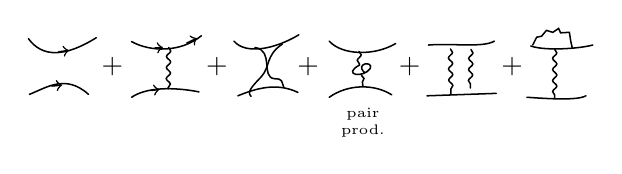
\begin{tikzpicture}[x=.62cm,y=.62cm,line width=.55pt,line cap=round,
 photon/.style={decorate,decoration={snake,amplitude=.75pt,segment length=4pt}}]
\draw (0,1.22) .. controls (.28,.84) and (.73,.83) .. (1.39,1.24);
\draw[->] (.62,.95)--(.83,.98);
\draw (.02,.08) .. controls (.38,.22) and (.76,.50) .. (1.23,.08);
\draw[->] (.48,.25)--(.69,.27);
\node at (1.72,.64) {$+$};
\begin{scope}[xshift=1.31cm]
\draw (0,1.16) .. controls (.38,.95) and (1.0,.93) .. (1.43,1.28);
\draw[->] (.48,1.03)--(.64,1.04); \draw[->] (1.13,1.13)--(1.34,1.23);
\draw (0,.02) .. controls (.37,.27) and (1.03,.20) .. (1.38,.13);
\draw[->] (.40,.16)--(.57,.18);
\draw[photon] (.76,1.04)--(.75,.19);
\end{scope}
\node at (3.86,.64) {$+$};
\begin{scope}[xshift=2.61cm]
\draw (0,1.17) .. controls (.24,.89) and (.83,1.00) .. (1.33,1.30);
\draw (.08,.05) .. controls (.45,.20) and (.87,.33) .. (1.31,.12);
\draw (.43,1.04) .. controls (.83,.98) and (.54,.43) .. (.83,.40)
 .. controls (1.01,.40) and (.97,.34) .. (1.02,.23);
\draw (.99,1.11) .. controls (.64,.87) and (.75,.65) .. (.56,.44)
 .. controls (.40,.27) and (.25,.13) .. (.35,.04);
\end{scope}
\node at (5.73,.64) {$+$};
\begin{scope}[xshift=3.82cm]
\draw (0,1.17) .. controls (.26,.88) and (.92,.86) .. (1.36,1.12);
\draw (0,.02) .. controls (.38,.29) and (.92,.30) .. (1.28,.07);
\draw[photon] (.61,.96)--(.62,.68);
\draw (.62,.68) .. controls (.25,.48) and (.70,.40) .. (.84,.61)
 .. controls (.91,.77) and (.52,.72) .. (.72,.53);
\draw[photon] (.66,.47)--(.69,.25);
\node[font=\tiny,align=center,below] at (.69,0) {pair\\prod.};
\end{scope}
\node at (7.81,.64) {$+$};
\begin{scope}[xshift=5.08cm]
\draw (0,1.09) .. controls (.48,1.13) and (1.12,1.03) .. (1.35,1.17);
\draw (-.03,.05)--(1.39,.10);
\draw[photon] (.45,1.01)--(.46,.08);
\draw[photon] (.87,1.00)--(.86,.21);
\end{scope}
\node at (9.91,.64) {$+$};
\begin{scope}[xshift=6.38cm]
\draw (0,1.07) .. controls (.28,.97) and (.96,1.01) .. (1.27,1.09);
\draw (.04,1.09)--(.12,1.25)--(.22,1.27)--(.32,1.39)--(.45,1.35)
 --(.57,1.43)--(.61,1.34)--(.79,1.35)--(.82,1.16)--(.85,1.03);
\draw[photon] (.49,1.00)--(.49,.01);
\draw (-.08,.02) .. controls (.36,-.01) and (.95,-.05) .. (1.13,.05);
\end{scope}
\end{tikzpicture}}\endgroup\par
The meeting of the strokes in the third sketch and the direction of the loop in the fourth are unclear.}
\end{GelfandAdjacentEvidence}
\begin{GelfandAdjacentEvidence}{GELFAND-P000608}{6}

\[
(\gamma_\mu p_\mu-m)K(p)=1
\]
\[
K(p)=\frac{\gamma_\mu p_\mu+m}{\underline p^{\,2}-m^2}
\]
\[
K(x,x')=\int K(p)e^{ip(x-x')}\,d^4p
\]
The pole is bypassed if we take \(K(p)=\dfrac{\gamma_\mu p_\mu+m}{\underline p^{\,2}-m^2+i0}\)
\Unclear{GELFAND-P000608}{pole-denominator}{The last mark is open and is read as zero.}
\end{GelfandAdjacentEvidence}
\begin{GelfandAdjacentEvidence}{GELFAND-P000608}{7}

\[
\underline{\underline p^{\,2}=E^2-\vec p^{\,2}}.
\]
\SourceFigure{GELFAND-P000608}{pole-axes}{%
\par\smallskip
\begingroup\color{black}\GelfandFitDiagram{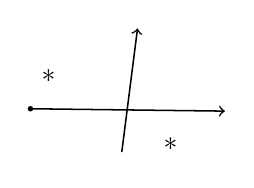
\begin{tikzpicture}[x=1cm,y=1cm,line width=.55pt]
\draw[->] (-1.25,.03)--(1.22,0);
\fill (-1.25,.03) circle (1pt);
\draw[->] (-.09,-.52)--(.11,1.05);
\node at (-1.02,.44) {$\ast$}; \node at (.53,-.42) {$\ast$};
\end{tikzpicture}}\endgroup\par}
\end{GelfandAdjacentEvidence}
\begin{GelfandAdjacentEvidence}{GELFAND-P000608}{8}

There are levels with neg. energy, nat. propagate backwards in time (pred. the existence of antiparticles).
\Unclear{GELFAND-P000608}{negative-energy-reading}{The abbreviation after “energy” tentatively reads “еств.” (nat.).}
\end{GelfandAdjacentEvidence}
\begin{GelfandAdjacentEvidence}{GELFAND-P000608}{9}


There is a unique choice of bypass leading to a consistent theory: — nor have antiparticles
\Unclear{GELFAND-P000608}{terminal-words}{The last two lines are close together. The reading “nor have antiparticles” is tentative.}
\end{GelfandAdjacentEvidence}



\Needspace{7\baselineskip}
\begin{GelfandAdjacentEvidence}{GELFAND-P000609}{1}
\SourcePage{GELFAND-P000609}{unlabelled}
\underline{Charge normalization}.

\(e\) — is this the obs. electron charge?

\dashuline{Scattering}: electrons exch. photons, force \(\sim e^2\)
\SourceFigure{GELFAND-P000609}{leading-exchange}{%
\par\smallskip
\begingroup\color{black}\GelfandFitDiagram{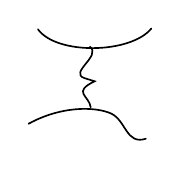
\begin{tikzpicture}[x=1cm,y=1cm,line width=.60pt,line cap=round]
\draw (0,1.35) .. controls (.24,1.02) and (1.18,1.04) .. (1.44,1.36);
\draw (-.12,.15) .. controls (.30,.38) and (.73,.37) .. (.93,.28)
 .. controls (1.12,.19) and (1.12,-.12) .. (1.37,-.04);
\draw (.66,1.13) .. controls (.81,1.01) and (.39,.80) .. (.59,.73)
 --(.72,.69) .. controls (.43,.55) and (.65,.51) .. (.67,.36);
\end{tikzpicture}}\endgroup\par}
\end{GelfandAdjacentEvidence}
\begin{GelfandAdjacentEvidence}{GELFAND-P000609}{2}


Correction: \(\sim e^4\).
\SourceFigure{GELFAND-P000609}{correction-loop}{%
\par\smallskip
\begingroup\color{black}\GelfandFitDiagram{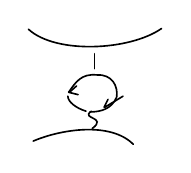
\begin{tikzpicture}[x=1cm,y=1cm,line width=.59pt,line cap=round]
\draw (-.04,1.58) .. controls (.31,1.26) and (1.25,1.31) .. (1.65,1.59);
\draw (.80,1.27)--(.80,1.08);
\draw (.47,.78) .. controls (.56,.91) and (.63,1.02) .. (.83,1.00)
 .. controls (1.02,1.01) and (1.10,.86) .. (1.08,.72)
 .. controls (1.02,.57) and (.88,.53) .. (.74,.53);
\draw (.69,.54) .. controls (.56,.58) and (.46,.66) .. (.46,.73);
\draw (.47,.78)--(.59,.75) (.48,.78)--(.57,.86);
\draw (.92,.59)--(.97,.69) (.93,.59)--(1.16,.73);
\draw (.76,.54) .. controls (.61,.44) and (.97,.47) .. (.77,.32);
\draw (.02,.16) .. controls (.37,.31) and (1.00,.41) .. (1.29,.12);
\end{tikzpicture}}\endgroup\par
The directions of the two arrow-like strokes on the loop are unclear. The visible gaps are retained.}
\end{GelfandAdjacentEvidence}


Obs. charge \(e_{\text{phys}}^2<e^2\).

In strong interact. theory the reverse holds \(g_{\text{phys}}^2>g^2\).
\[
\rule{1.8em}{.4pt}\;\boldsymbol{\cdot}\;\rule{1.8em}{.4pt}
\]


\Needspace{7\baselineskip}
\begin{GelfandAdjacentEvidence}{GELFAND-P000610}{1}
\SourcePage{GELFAND-P000610}{unlabelled}
\underline{\underline{22.9.75.}}\qquad\underline{Gelfand Sem.}

\SourceFigure{GELFAND-P000610}{scan-comment-mark}{%
\par\smallskip
\begingroup\color{black}\GelfandFitDiagram{
\begin{tikzpicture}[x=1cm,y=1cm,line width=.55pt]
\draw[fill=yellow,rounded corners=2pt] (0,.17)--(0,.74)--(.84,.74)--(.84,.17)--(.42,.17)--(.22,0)--(.26,.17)--cycle;
\draw (.14,.59)--(.70,.59) (.14,.46)--(.70,.46) (.14,.33)--(.56,.33);
\end{tikzpicture}}\endgroup\par
Yellow comment icon in the upper right margin of the digitized frame.}
\end{GelfandAdjacentEvidence}
\begin{GelfandAdjacentEvidence}{GELFAND-P000610}{2}


\underline{Gelfand on Atiyah’s res.}

\(\mathfrak A\) — all oper. in Hilb. sp., \(\mathcal K\) — comp. oper.
\[
\mathfrak A/\mathcal K=\mathfrak B.
\]
When are \(B_1,B_2\in\mathfrak B\) unitarily equivalent?

This is [crossed out] \uwave{Brown, Douglas, Fillmore} (Lect. Notes, \(N=\ldots\))
\Unclear{GELFAND-P000610}{cancel-before-brown}{An entry before the surnames is crossed out. It may read “Все” (all).}
\end{GelfandAdjacentEvidence}
\begin{GelfandAdjacentEvidence}{GELFAND-P000610}{3}


a) spectra coincide (ess.)

b) indices coincide in [crossed out] \(\forall\) conn. comp. of the complement
\Incomplete{GELFAND-P000610}{cancel-indices}{An entry before the quantifier is crossed out.}
\end{GelfandAdjacentEvidence}
\begin{GelfandAdjacentEvidence}{GELFAND-P000610}{4}


\underline{Thm. 2.} [crossed out] Let \(X\) — be a compact space,
\[
\underset{\substack{\uparrow\\\text{set of embeddings of }C(X)\text{ in }\mathfrak B.}}{\operatorname{Ext}(X)}\cong K_1(X)
\]
\Incomplete{GELFAND-P000610}{cancel-theorem}{An entry before “Let” is crossed out.}
\end{GelfandAdjacentEvidence}
\begin{GelfandAdjacentEvidence}{GELFAND-P000610}{5}


\[\rule{1.8em}{.4pt}\;\boldsymbol{\cdot}\;\rule{1.8em}{.4pt}\]
\dashuline{Moser} — \uwave{Korteweg–de Vries}
\[\rule{1.8em}{.4pt}\;\boldsymbol{\cdot}\;\rule{1.8em}{.4pt}\]
\dashuline{Kostant}
\[
\psi(x)=\prod_{n=1}^{\infty}(1-x^n);\qquad
\psi(x)^{-1}=\sum_{n=0}^{\infty}p(n)x^n
\]
(\(p(n)\) — number of part. of \(n\)).

This is
\[
\psi(x)=\sum(-1)^n x^{\frac{n^2-3n}{2}}
\]
\Unclear{GELFAND-P000610}{euler-exponent}{The exponent is written \((n^2-3n)/2\).}
\end{GelfandAdjacentEvidence}
\begin{GelfandAdjacentEvidence}{GELFAND-P000610}{6}


\noindent\makebox[0pt][r]{\(\bullet\)\hspace{.7em}}“The most remarkable formula in all of mathematics” (Jacobi).
\Unclear{GELFAND-P000610}{function-abbreviation}{The heavily overwritten abbreviation after “remarkable” tentatively reads “ф-ла” (formula).}
\end{GelfandAdjacentEvidence}
\begin{GelfandAdjacentEvidence}{GELFAND-P000610}{7}

\[
(\psi(x))^3=\sum_{n=0}^{\infty}(-1)^n(2n+1)x^{\frac{n(n+1)}2}
\]
\[
\eta(x)=x^{1/24}\cdot\psi(x).
\]
\[
\eta^{24}(x)=\sum\tau(n)x^n,\qquad\tau(n)\text{ — Ramanujan’s function}
\]
\(\psi^{10}(x)\) exists too

\underline{Manin}: if 6 different fns., obt. from different considerations
\[
\eta(x)^{\square}=\sum\ldots
\]
Macdonald found powers for which it makes sense:
These are the \(\dim\) of compact Lie groups.
\[
\psi(x)^{\dim K}=\sum_\lambda\text{[crossed out]}\ \chi_\lambda(a)\,\dim V_\lambda\cdot x^{\text{(depends on }\lambda\text{)}}
\]
\Incomplete{GELFAND-P000610}{cancel-character}{An entry after the summation sign and before \(\chi_\lambda(a)\) is crossed out.}
\end{GelfandAdjacentEvidence}
\begin{GelfandAdjacentEvidence}{GELFAND-P000610}{8}

\(a\in K\), \(\chi_\lambda(a)=\pm1\) or \(0\)

Kostant: \(\operatorname{Sp}(-\Delta+a)^{-s}\) etc.

\dashuline{Internal [ч-ие] G.}: \uwave{\(\psi(x)^z\)} — ?\qquad \((z\in\mathbb C)\)
\Unclear{GELFAND-P000610}{inner-abbreviation}{The middle abbreviation tentatively reads “ч-ие”.}
\end{GelfandAdjacentEvidence}
\begin{GelfandAdjacentEvidence}{GELFAND-P000610}{9}

\[\rule{1.8em}{.4pt}\;\boldsymbol{\cdot}\;\rule{1.8em}{.4pt}\]
\underline{\underline{Polyakov}}. (continued).

\underline{References}:
\[
\text{\underline{quant. mech.}}\quad\left\{\begin{array}{@{}l@{}}
\text{1) \uwave{Landau and Lifshitz} (quant. mechanics).}\ (\approx5\text{–}7\ \text{chapters})\\
\text{2) \uwave{Dirac}}\\
\text{3) \uwave{Feynman} (for schoolchildren)}\\
\text{4) \uwave{Feynman}. Path integrals}
\end{array}\right.
\]
\Unclear{GELFAND-P000610}{bibliography-count}{The word after “5–7” tentatively reads “глав” (chapters).}
\end{GelfandAdjacentEvidence}


\underline{Quant. field theory}: 1st part of vol. \underline{IV}\quad\dashuline{Berestetskii, Lifshitz, Pitaevskii}


\Needspace{7\baselineskip}
\begin{GelfandAdjacentEvidence}{GELFAND-P000611}{1}
\SourcePage{GELFAND-P000611}{unlabelled}
\(e(x)\) — field (bispinors)
\[
\mathcal L_{\mathrm{free}}=\bar e\,i\gamma_\mu\partial_\mu e
-m\bar e e+\frac1{4e^2}F_{\mu\nu}^2
\]
\[
\mathcal L_{\mathrm{int}}=\ldots\bar e\gamma_\mu e A_\mu\ldots
\qquad\text{cont. 3-… terms}
\]
\Unclear{GELFAND-P000611}{interaction-abbreviation}{The abbreviation after “3-” is uncertain.}
\end{GelfandAdjacentEvidence}
\begin{GelfandAdjacentEvidence}{GELFAND-P000611}{2}

\[\rule{1.8em}{.4pt}\;\boldsymbol{\cdot}\;\rule{1.8em}{.4pt}\]
\dashuline{Localization of large int. symmetries — weak interaction.}
\Unclear{GELFAND-P000611}{heading-abbreviations}{“б-их вн.” tentatively reads “large internal”.}
\end{GelfandAdjacentEvidence}
\begin{GelfandAdjacentEvidence}{GELFAND-P000611}{3}

\[
\begin{aligned}
\mathcal L={}&\bar e_L i\gamma_\mu\partial_\mu e_L
+\bar e_R i\gamma_\mu\partial_\mu e_R
+\bar\nu_L i\gamma_\mu\partial_\mu\nu_L+\\
&+\begin{pmatrix}e\to\mu\\ \nu_L\to\nu'_L\end{pmatrix}
+m(\bar e_L e_R+\bar e_R e_L).
\end{aligned}
\]
(all leptons)\quad\(\downarrow\)

\(\nu'_L\) — \(\mu\)-meson neutrino
\[
\mathcal L=\bar e_L i\gamma_\mu\partial_\mu e_L
+\bar\nu_L i\gamma_\mu\partial_\mu\nu_L
+\bar e_R i\gamma_\mu\partial_\mu e_R
\]
\[
\left\{
\begin{aligned}
\begin{pmatrix}e'_L\\\nu'_L\end{pmatrix}
&=U\begin{pmatrix}e_L\\\nu_L\end{pmatrix}
\qquad SU_L(2)\\
e'_R&=e_R
\end{aligned}
\right.
\]
\hfill\(\bullet\)

A new symmetry gr. \(SU(2)\) arises, and also \(U(1)\)
\[
F=SU_L(2)\times U_R(1)\times U_L(1)
\quad\text{— overall lepton group.}
\]
\[
\begin{pmatrix}e_L\\\nu_L\end{pmatrix}
\overset{U_L(1)}{\longrightarrow}
e^{i\gamma}\begin{pmatrix}e_L\\\nu_L\end{pmatrix}
\]
\Unclear{GELFAND-P000611}{phase-letter}{The letter in the phase tentatively reads \(\gamma\), possibly \(\delta\).}
\end{GelfandAdjacentEvidence}
\begin{GelfandAdjacentEvidence}{GELFAND-P000611}{4}


\dashuline{Localization}

\Incomplete{GELFAND-P000611}{cancel-left}{The crossed-out entry in a box in the left margin is illegible.}
\end{GelfandAdjacentEvidence}
\begin{GelfandAdjacentEvidence}{GELFAND-P000611}{5}


[Crossed out: \sout{\(A_\mu\) … electromagn. field}.]
\Unclear{GELFAND-P000611}{cancel-a}{A mark between \(A_\mu\) and “electromagn. field” is obscured by the crossing-out.}
\end{GelfandAdjacentEvidence}
\begin{GelfandAdjacentEvidence}{GELFAND-P000611}{6}


Covar. derivative for \(SU(2)\).
\qquad \(\bar\tau\) — Pauli matr. (3 in all)
\[
\begin{pmatrix}e'_L\\\nu'_L\end{pmatrix}
=e^{i\frac{\vec\tau\vec\alpha(x)}2}
\begin{pmatrix}e_L\\\nu_L\end{pmatrix},
\qquad E'=e^{i\frac{\bar\tau\bar\alpha(x)}2}E
\]
\Unclear{GELFAND-P000611}{doublet-overwrite}{The lower letter on the left and the lower subscript on the right are overwritten.}
\end{GelfandAdjacentEvidence}
\begin{GelfandAdjacentEvidence}{GELFAND-P000611}{7}

Infinitesim.:
\[
E'=\left(1-\frac i2(\bar\tau\bar\alpha)\right)E
\]
\Unclear{GELFAND-P000611}{finite-infinitesimal-sign}{The finite exponent is written with an implicit plus sign. A minus sign is visible in the infinitesimal expression.}
\end{GelfandAdjacentEvidence}

\[
\partial_\mu E'=
\left(1-\frac i2(\bar\tau\bar\alpha)\right)\partial_\mu E
-\frac i2(\bar\tau\partial_\mu\bar\alpha)E
\]
\[
\fbox{$\displaystyle\nabla_\mu E
=\partial_\mu E+\frac i2(\vec\tau\vec A_\mu)E$}
\]
\[
E'=e^{i\frac{\bar\tau\bar\alpha(x)}2}E
\]
\[
\nabla_\mu E'=e^{i\frac{\bar\tau\bar\alpha}2}\nabla_\mu E
\]
Here 3 massless particles arise


\Needspace{7\baselineskip}
\begin{GelfandAdjacentEvidence}{GELFAND-P000612}{1}
\SourcePage{GELFAND-P000612}{unlabelled}
one can write directly
\[
\nabla_\mu E^\delta=\partial_\mu E^\delta+A_\mu^{\delta\beta}E^\beta
\]
\Unclear{GELFAND-P000612}{upper-component-index}{The superscript tentatively reads \(\delta\), possibly \(\gamma\).}
\end{GelfandAdjacentEvidence}
\begin{GelfandAdjacentEvidence}{GELFAND-P000612}{2}

and we look at how \(A\) transforms so that \(\nabla_\mu E^\delta\) transforms like \(E^\delta\).

\[
\begin{aligned}
\mathcal L_{\mathrm{int}}={}&(\bar e_i\gamma_\mu\nu_e)A_\mu^{(-)}
+(\bar\nu_e\gamma_\mu e_i)A_\mu^{(+)}\\
&+(\bar e_L\gamma_\mu e_L-\bar\nu_L\gamma_\mu\nu_L)A_\mu^3
\end{aligned}
\]
\Unclear{GELFAND-P000612}{weak-electron-index}{The electron index in the first two terms is written with a dotted \(i\).}
\end{GelfandAdjacentEvidence}
\begin{GelfandAdjacentEvidence}{GELFAND-P000612}{3}

where
\[
A_\mu^\pm=A_\mu^1\pm iA_\mu^2
\]
Example of weak interaction: \(\mu^-\to e^-,\bar\nu_e,\nu_\mu.\)
\[
\mathcal L=\bar E\left(i\gamma_\mu\frac{\partial E}{\partial x_\mu}\right)
+\underset{\mathcal L_{\mathrm{int}}}{\tikz[baseline=(term.base)]{
\node[inner sep=0pt] (term) {$\bar E\gamma_\mu\vec\tau E\vec A_\mu$};
\draw ([yshift=-.2ex]term.south west) -- ([yshift=-.75ex]term.south west)
-- ([yshift=-.75ex]term.south east) -- ([yshift=-.2ex]term.south east);
}}
+\bar e_R i\gamma_\mu\partial_\mu e_R
\]
\Unclear{GELFAND-P000612}{lagrangian-mark}{There is a separate short stroke with dots to the left of \(\mathcal L\). Its meaning is uncertain.}
\end{GelfandAdjacentEvidence}
\begin{GelfandAdjacentEvidence}{GELFAND-P000612}{4}

\Incomplete{GELFAND-P000612}{cancel-underbrace}{An entry beneath the left side of the bracket is crossed out.}
\end{GelfandAdjacentEvidence}
\begin{GelfandAdjacentEvidence}{GELFAND-P000612}{5}

\Incomplete{GELFAND-P000612}{cancel-right}{A separate crossed-out entry in the right margin is illegible.}
\end{GelfandAdjacentEvidence}
\begin{GelfandAdjacentEvidence}{GELFAND-P000612}{6}


\[\rule{1.8em}{.4pt}\;\boldsymbol{\cdot}\;\rule{1.8em}{.4pt}\]
We also localize the r. field
\Unclear{GELFAND-P000612}{right-field-abbreviation}{The abbreviation “пр.” tentatively means “right”.}
\end{GelfandAdjacentEvidence}
\begin{GelfandAdjacentEvidence}{GELFAND-P000612}{7}

\[
\begin{aligned}
&\bar E\left(i\gamma_\mu\frac{\partial E}{\partial x_\mu}\right)
+\bar E\gamma_\mu\vec\tau E\vec A_\mu
+\bar e_R i\gamma_\mu\partial_\mu e_R\\
&\qquad+\bar e_R\gamma_\mu e_R B_\mu
\end{aligned}
\]
\[
A_\mu=A_\mu^3\cos\theta+B_\mu\sin\theta
\]
\[\boldsymbol{\cdot}\;\cdot\;\cdot\;\cdot\;\cdot\;\cdot\;{\scriptscriptstyle-}\;
\cdot\;\cdot\;\cdot\;\cdot\;\cdot\]
Next time — \(\approx\) \underline{in 3 weeks.}

\textbf{12 quarks:} \uwave{4 flavors and 3 colors.}

\SourceFigure{GELFAND-P000612}{scan-comment-mark}{%
\par\smallskip
\begingroup\color{black}\GelfandFitDiagram{
\begin{tikzpicture}[x=1cm,y=1cm,line width=.55pt]
\draw[fill=yellow,rounded corners=2pt] (0,.17)--(0,.74)--(.84,.74)--(.84,.17)--(.42,.17)--(.22,0)--(.26,.17)--cycle;
\draw (.14,.59)--(.70,.59) (.14,.46)--(.70,.46) (.14,.33)--(.56,.33);
\end{tikzpicture}}\endgroup\par
Yellow comment icon to the right of the quark entry in the digitized frame.}
\end{GelfandAdjacentEvidence}

\[\rule{1.8em}{.4pt}\;\boldsymbol{\cdot}\;\rule{1.8em}{.4pt}\]


\Needspace{7\baselineskip}
\begin{GelfandAdjacentEvidence}{GELFAND-P000613}{1}
\SourcePage{GELFAND-P000613}{unlabelled}
\uuline{29.9.75.}\qquad\uuline{Gelfand Sem.}

\uuline{Yu. I. Manin.}
\[
x\prod_{n=1}^\infty(1-x^n)^{24}=\sum_{n=1}^\infty\tau(n)x^n;
\qquad \tau\text{ — Ramanujan’s function}.
\]
\underline{I. M. Gelfand}. (and Dikii)

\(\infty\)\uwave{-dimensional Lie algebra, more remarkable than all the Cartan ones}.

Elements — polynomials \(P(u,u',\ldots,u^{(n)})\) in any number of variables.

\(P\overset{\prime\prime}{[}u]\), where \(u=\{u,u',\ldots,u^{(n)},\,\cdot\,\}\)
\Unclear{GELFAND-P000613}{formal-variable-mark}{Two strokes stand above the left square bracket.}
\end{GelfandAdjacentEvidence}
\begin{GelfandAdjacentEvidence}{GELFAND-P000613}{2}


There is a notion of
\[
\frac{d}{dx}P(u,u',\ldots,u^{(n)})
=\sum_{i=0}^\infty\frac{\partial P}{\partial u^{(i)}}\cdot u^{(i+1)}
\]
There is multiplication (algebr.)

Unexpectedly, there is a notion of the \underline{commutator}:
\[
[P,Q]=\sum_{k=0}^\infty
\left[\left(\frac{d}{dx}\right)^kP\cdot\frac{\partial Q}{\partial u^{(k)}}
-\left(\frac{d}{dx}\right)^kQ\cdot\frac{dP}{du^{(k)}}\right]
\]
\Unclear{GELFAND-P000613}{commutator-separator}{The mark after \(Q\) reads as a multiplication dot. The last fraction uses \(d\).}
\end{GelfandAdjacentEvidence}
\begin{GelfandAdjacentEvidence}{GELFAND-P000613}{3}

\Unclear{GELFAND-P000613}{cancelled-speaker}{A short entry before the surname is crossed out.}
\end{GelfandAdjacentEvidence}
\begin{GelfandAdjacentEvidence}{GELFAND-P000613}{4}

\Incomplete{GELFAND-P000613}{cancelled-speaker-loss}{The crossed-out entry cannot be read in full.}
\end{GelfandAdjacentEvidence}
\begin{GelfandAdjacentEvidence}{GELFAND-P000613}{5}


\uuline{Povzner}. This alg. is connected with the eq. \(\dfrac{\partial u}{\partial t}=\dfrac{\partial u}{\partial x}\).
Can be connected with \(\forall\) eq.
\[
\frac{\partial u}{\partial t}=a(u,u_x,\ldots).
\]
Consider fns. \(F(u,u_x,\ldots)\) and the operator
\[
a[F(u,u_x,\ldots)]=aF_u+\left(\frac{d}{dx}a\right)F_{u_x}
+\frac{d^2a}{dx^2}F_{u_{xx}}+\ldots
\]
The operator is det. by the fn. \(a\) and an algebra is built from these oper.
\[
[a,b]=a[b]-b[a]\text{ — the same algebra}.
\]
\[\rule{1.8em}{.4pt}\;\boldsymbol{\cdot}\;\rule{1.8em}{.4pt}\]
Here the natural repr. of this algebra is indicated.
\Unclear{GELFAND-P000613}{representation-marginal-mark}{A mark to the left of “Here” is blacked out.}
\end{GelfandAdjacentEvidence}
\begin{GelfandAdjacentEvidence}{GELFAND-P000613}{6}

\[\rule{1.8em}{.4pt}\;\boldsymbol{\cdot}\;\rule{1.8em}{.4pt}\]
\uuline{Manin}. 6 expressions for Ramanujan’s fn. \(\tau(n)\) (not obt. by a finite algorithm).

\textcircled{\scriptsize +}\quad\textcircled{\scriptsize 1}\quad\underline{Definition} \(\Rightarrow\)
\[
\tau(n)=\sum(-1)^k
\]
\[
\begin{gathered}
n-1=n_1+\ldots+n_k,\qquad n_i\ge1\\
n_1\le n_2\le\ldots\le n_k
\end{gathered}
\]
in a row \(\le24\) equality signs.

\textcircled{\scriptsize +}\quad\textcircled{\scriptsize 2}\quad\uwave{Macdonald} (\uwave{Dyson})
\[
\tau(n)=\frac1{1!2!3!4!}\sum\prod_{i<j}(u_i-u_j)
\]
\Unclear{GELFAND-P000613}{vandermonde-relation}{The index condition below the product tentatively reads \(i<j\).}
\end{GelfandAdjacentEvidence}
\begin{GelfandAdjacentEvidence}{GELFAND-P000613}{7}

\[
10n=\sum_{i=1}^5u_i^2,\qquad\sum u_i=0,\qquad u_i\equiv i\bmod5
\]

\(\left(\begin{smallmatrix}+\\+\end{smallmatrix}\right)\)
\quad\textcircled{\scriptsize 3}\quad\uwave{Ramanujan}
\[
\tau(n)=\frac{65}{756}\sigma_{11}(n)+\frac{691}{756}\sigma_5(n)
-\frac{691}{3}\sum_{m=1}^{n-1}\sigma_5(m)\sigma_5(n-m)
\]
\Unclear{GELFAND-P000613}{ramanujan-denominator}{The last digit of the first denominator is overwritten and reads as 6.}
\end{GelfandAdjacentEvidence}
\begin{GelfandAdjacentEvidence}{GELFAND-P000613}{8}

\Unclear{GELFAND-P000613}{ramanujan-convolution}{The argument in the final factor reads \(n-m\).}
\end{GelfandAdjacentEvidence}

\(\sigma_k(n)\) — \(\sum\) of the \(k\)th powers of the divisors of \(n\).

\underline{Corollary:} \(\tau(n)\equiv\sigma_{11}(n)\bmod691\).
(guessed by Ramanujan).


\Needspace{7\baselineskip}
\begin{GelfandAdjacentEvidence}{GELFAND-P000614}{1}
\SourcePage{GELFAND-P000614}{unlabelled}
\textcircled{\scriptsize 4}\quad Int. quad. forms with \(\det=1\) in 24 variables.
\hfill 2 in all.

\(\left(\begin{smallmatrix}+\\+\end{smallmatrix}\right)\)
\qquad Let \(Q_{24}\) — one of them.
\Unclear{GELFAND-P000614}{form-count}{The line reads “2 in all”.}
\end{GelfandAdjacentEvidence}
\begin{GelfandAdjacentEvidence}{GELFAND-P000614}{2}

\[
\tau(n)=\alpha\left(\sum_{Q_{24}=n}1\right)-\beta\sigma_{11}(n)
\]
(\(\alpha,\beta\) computed from \(n=1\) and \(2\)).

\textcircled{\scriptsize 5}\quad (Manin)
\hspace{1em}\(\left(\begin{smallmatrix}+\\+\end{smallmatrix}\right)\)
\[
\tau(n)=\sigma_{11}(n)-\sum_{n=\Delta\Delta'+\delta\delta'}'
\left[(\Delta^8\delta^2-\Delta^2\delta^8)
+\frac{691}{6}(\Delta^6\delta^4-\Delta^4\delta^6)\right],
\]
\Unclear{GELFAND-P000614}{manin-primed-sum}{There is a prime on the summation sign.}
\end{GelfandAdjacentEvidence}
\begin{GelfandAdjacentEvidence}{GELFAND-P000614}{3}

\[
\begin{gathered}
\Delta>\delta>0,\quad\text{and }\bigl[\,\Delta'>\delta'>0\quad(\text{integers})\\
\text{or }\Delta\mid n,\quad \Delta'=\frac n\Delta,\quad
\delta'=0,\quad0<\frac\delta\Delta\le\frac12\,\bigr].
\end{gathered}
\]

\textcircled{\scriptsize 6}\quad
\(\left(\begin{smallmatrix}+\\+\\+\end{smallmatrix}\right)\)
\[
\sum p(n)x^n=\prod_{n=1}^\infty(1-x^n)^{-1}
\]
(\(p(n)\) — number of partitions of \(n\) into any number of summands).
\[
\Rightarrow\quad \sum\tau(n)x^n=x\left(\sum_{n=1}^{\infty}p(n)x^n\right)^{-24}
\]
\Unclear{GELFAND-P000614}{partition-inner-start}{The lower limit of the inner sum is written \(n=1\).}
\end{GelfandAdjacentEvidence}
\begin{GelfandAdjacentEvidence}{GELFAND-P000614}{4}

Using \(p(n)\), find \(\tau(n)\) recursively.

Hardy–Ramanujan–Rademacher formula
\[
p(n)=\frac1{\sqrt3}\sum_{k=1}^{\infty}\frac1{\sqrt k}
\sum_{\substack{h\bmod k\\(h,k)=1}}
\omega_{h,k}e^{-2\pi i n\frac1k}\cdot
\frac d{dn}\frac{\operatorname{sh}\frac\pi{6k}\sqrt{24n-1}}
{\frac\pi{6k}\sqrt{24n-1}}
\]
\Unclear{GELFAND-P000614}{hrr-omega-exponential}{The exponent is written with \(1/k\).}
\end{GelfandAdjacentEvidence}
\begin{GelfandAdjacentEvidence}{GELFAND-P000614}{5}

\(\omega_{h,k}^{24}=1\) there are also explicit formulas for \(\omega_{h,k}\).

Hardy–Ramanuj. wrote [crossed out] \(\operatorname{sh}\to e^{\ldots}\).
\Incomplete{GELFAND-P000614}{hrr-cancelled-prefix}{A short entry before “sh” is crossed out.}
\end{GelfandAdjacentEvidence}
\begin{GelfandAdjacentEvidence}{GELFAND-P000614}{6}

[Below \(\operatorname{sh}\to e^{\ldots}\): diverges.]
but if one truncates at the \(\sqrt n\) term, it approximates well.
One has to stop at \(\sqrt n\) terms.
Each of these formulas is part of an infinite series of formulas.

\textcircled{\scriptsize 7}\quad
\(\left(\begin{smallmatrix}+\\+\end{smallmatrix}\right)\)
\qquad \uuline{\(\tau(mn)=\tau(m)\tau(n)\)}, \((m,n)=1\)

(not apparent from the formulas).
\[
\tau(p)=\theta_p+\bar\theta_p,\qquad\theta_p\bar\theta_p=p^{11}
\quad\Rightarrow
\]
\begin{center}
\uuline{\(\tau(p^a)=\theta_p^a+\bar\theta_p^a.\)}
\end{center}
\Unclear{GELFAND-P000614}{theta-power}{The doubly underlined formula is given as written.}
\end{GelfandAdjacentEvidence}
\begin{GelfandAdjacentEvidence}{GELFAND-P000614}{7}

One can substitute in each formula and obtain new identities.

\textcircled{\scriptsize 8}\quad
\(\left(\begin{smallmatrix}+\\+\\+\\+\end{smallmatrix}\right)\)
\qquad From this [circled insertion: the suspicion that] \(\tau\) — trace of a representation (much harder) — Serre, Deligne.
\Unclear{GELFAND-P000614}{suspicion-insertion}{The circled insertion reads “the suspicion that”.}
\end{GelfandAdjacentEvidence}
\begin{GelfandAdjacentEvidence}{GELFAND-P000614}{8}

Grothendieck, Weil, Kuga, Sato, [crossed out] Rankin.
\Incomplete{GELFAND-P000614}{cancelled-author}{The crossed-out entry before Rankin is illegible.}
\end{GelfandAdjacentEvidence}
\begin{GelfandAdjacentEvidence}{GELFAND-P000614}{9}

An \(\ell\)-adic repr.
\[
\operatorname{Gal}_{\{\ell\}}(\bar Q/Q)\longrightarrow Q_\ell^2
\]
(ramif. only at \(\ell\)).
The trace is taken of the Frobenius autom. gen. by \(p\).

From this it was possible to prove that \uuline{\(\theta_p\) are purely imaginary} (nonreal)
\Unclear{GELFAND-P000614}{theta-imaginary}{The manuscript reads “purely imaginary”.}
\end{GelfandAdjacentEvidence}

\(\longrightarrow\) The longest thm. in modern mathematics (Deligne’s estimate: 2,000 pages).


\Needspace{7\baselineskip}
\begin{GelfandAdjacentEvidence}{GELFAND-P000615}{1}
\SourcePage{GELFAND-P000615}{unlabelled}
\underline{Levels of difficulty.}
\[
\begin{array}{cl}
+&\text{combinatorics}\\
++&\text{modular forms}\\
+++&\text{complex analysis}\\
++++&\text{alg. geom. and the like, étale cohom. and so on}\\\hline
\end{array}
\]
\[\rule{1.8em}{.4pt}\;\boldsymbol{\cdot}\;\rule{1.8em}{.4pt}\]

\underline{How it is obtained.}
\[
\eta(z)=e^{\frac{2\pi inz}{24}}\prod(1-e^{2\pi inz})
\]
\Unclear{GELFAND-P000615}{eta-prefactor}{The prefactor exponent is written \(2\pi inz/24\).}
\end{GelfandAdjacentEvidence}
\begin{GelfandAdjacentEvidence}{GELFAND-P000615}{2}

Set \(x=e^{\frac{2\pi inz}{24}}\).
\Unclear{GELFAND-P000615}{x-definition}{The heavily inked mark between \(i\) and \(z\) tentatively reads \(n\). The denominator is overwritten.}
\end{GelfandAdjacentEvidence}
\begin{GelfandAdjacentEvidence}{GELFAND-P000615}{3}

The fn. behaves [crossed out] well under the substitution
\(z\to\dfrac{az+b}{cz+d}\),
\(\begin{vmatrix}a&b\\c&d\end{vmatrix}=1\).
\Incomplete{GELFAND-P000615}{verb-cancelled}{Short strokes after the verb are crossed out.}
\end{GelfandAdjacentEvidence}
\begin{GelfandAdjacentEvidence}{GELFAND-P000615}{4}

\[
\begin{aligned}
\eta(z+1)&=e^{\pi i/12}\eta(z),\\
\eta(-1/z)&=\sqrt{z/i}\,\eta(z).
\end{aligned}
\]
or \(\eta^{24}(\tau)(d\tau)^6\) — inv. under frac.-lin. subst..
\Unclear{GELFAND-P000615}{eta-differential}{The exponent on \(d\tau\) is written \(6\).}
\end{GelfandAdjacentEvidence}
\begin{GelfandAdjacentEvidence}{GELFAND-P000615}{5}


Loss of inf. — \(\sqrt[24]{\ldots}=\omega_{c,d}\) — the same ones.
\[
\begin{pmatrix}a,&\bar b\\c,&d\end{pmatrix}
\]
\Unclear{GELFAND-P000615}{matrix-mark}{In the matrix below “Loss of inf.” there is a separate stroke over \(b\).}
\end{GelfandAdjacentEvidence}
\begin{GelfandAdjacentEvidence}{GELFAND-P000615}{6}

Fns. of this kind (modular) form a ring with 2 generators, and one must write them in terms of the generators, [crossed out \sout{or}]
Identity in the ring \(\Rightarrow\) equality of Fourier coeffs.
(\(\Rightarrow\) \textcircled{\scriptsize 3}, \textcircled{\scriptsize 4}).
\Unclear{GELFAND-P000615}{or-cancelled}{A word above the line is crossed out. It tentatively reads “or”.}
\end{GelfandAdjacentEvidence}
\begin{GelfandAdjacentEvidence}{GELFAND-P000615}{7}


\uuline{Pure algebra:}
\[
\left\{\varphi(z)\mathrel{\Big|}\sum_{n=0}^\infty a_ne^{2\pi inz}\right\},
\qquad
\exists k:\quad \varphi(z)dz^k\mathrel{\Big|}\begin{pmatrix}a&b\\c&d\end{pmatrix}
=\varphi(z)dz^k.
\]
\(\longleftarrow\) converg. series for \(\operatorname{Im}z>0\).

\underline{Thm.:} the ring \(\Phi=C[E_4,E_6]\).
\[
\begin{aligned}
a_n|_{E_4}&=\sigma_3(n)\\
a_n|_{E_6}&=\sigma_5(n)
\end{aligned}
\Bigg\Vert\qquad \sigma_3\text{ — sums of cubes of divisors}.
\]
\[\rule{1.8em}{.4pt}\;\boldsymbol{\cdot}\;\rule{1.8em}{.4pt}\]

\underline{H. R. R.} (formula 6).
\[
\sum p(n)e^{2\pi inz}=\frac1{\prod(1-e^{2\pi izn})}.
\]
Sing. points on the boundary of convergence (poles of order \(\infty\) at rat. points).

Rademacher’s integr. contour: at \(\forall\) rat. point, circles of a given radius.
\SourceFigure{GELFAND-P000615}{circle-contour}{%
\par\smallskip
\begingroup\color{black}\GelfandFitDiagram{\begin{tikzpicture}[x=1.65cm,y=1.65cm,line width=.55pt]
\draw (-.51,0)--(1.49,.015);
\draw (0,0) .. controls (-.24,0) and (-.49,.28) .. (-.49,.48)
 .. controls (-.51,.82) and (-.32,.94) .. (.03,.97)
 .. controls (.25,1.01) and (.49,.71) .. (.5,.51)
 .. controls (.50,.29) and (.26,0) .. (0,0);
\draw (1,0) .. controls (.78,0) and (.51,.21) .. (.51,.44)
 .. controls (.49,.67) and (.75,.92) .. (1.04,.91)
 .. controls (1.28,.93) and (1.48,.71) .. (1.48,.51)
 .. controls (1.48,.24) and (1.21,0) .. (1,0);
\draw (.5,.13) ellipse [x radius=.115,y radius=.115];
\draw (.30,.012) .. controls (.33,.17) and (.41,.10) .. (.42,.012);
\draw (.59,.014) .. controls (.63,.115) and (.68,.105) .. (.71,.014);
\node[below] at (0,0) {\(0\)};
\node[below] at (.5,0) {\(\tfrac12\)};
\node[below] at (1,0) {\(1\)};
\end{tikzpicture}}\endgroup\par
The exact shape of the short arcs near the small circle is uncertain.}
\end{GelfandAdjacentEvidence}
\begin{GelfandAdjacentEvidence}{GELFAND-P000615}{8}

\SourceFigure{GELFAND-P000615}{contour-first-approximation}{%
\par\smallskip
\begingroup\color{black}\GelfandFitDiagram{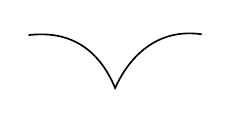
\begin{tikzpicture}[x=1.1cm,y=1.05cm,line width=.6pt]
\draw (0,.64) .. controls (.47,.70) and (.81,.48) .. (1,0)
 .. controls (1.20,.46) and (1.55,.72) .. (2,.65);
\end{tikzpicture}}\endgroup\par
— 1st approx.}
\end{GelfandAdjacentEvidence}
\begin{GelfandAdjacentEvidence}{GELFAND-P000615}{9}

\SourceFigure{GELFAND-P000615}{contour-second-approximation}{%
\par\smallskip
\begingroup\color{black}\GelfandFitDiagram{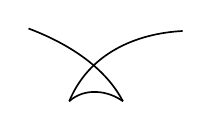
\begin{tikzpicture}[x=1.1cm,y=1.05cm,line width=.6pt]
\draw (0,.88) .. controls (.38,.73) and (.86,.46) .. (1.09,0);
\draw (.47,0) .. controls (.70,.58) and (1.24,.82) .. (1.78,.85);
\draw (.47,0) .. controls (.65,.17) and (.92,.13) .. (1.09,0);
\end{tikzpicture}}\endgroup\par
— 2nd approx.}
\end{GelfandAdjacentEvidence}
\begin{GelfandAdjacentEvidence}{GELFAND-P000615}{10}

etc.
\par\smallskip\noindent\rule{\linewidth}{.35pt}\par

Special case of Macdonald’s formulas in the form transformed by Kostant:
\[
\varphi(x)=\prod_{n=1}^\infty(1-x^n),\qquad
\varphi(x)=\sum_{\lambda\in D}\chi_\lambda(a)\dim V_\lambda\,x^{c(\lambda)}.
\]
\Incomplete{GELFAND-P000615}{kostant-cancelled}{A short entry beneath the product is heavily crossed out.}
\end{GelfandAdjacentEvidence}

[under \(\lambda\in D\): highest weights of irred. reps.; under \(\chi_\lambda(a)\): \(0,\pm1\).]
\[
c(\lambda)=(\lambda+\rho,\lambda+\rho)-(\rho,\rho).
\]


\Needspace{7\baselineskip}
\begin{GelfandAdjacentEvidence}{GELFAND-P000616}{1}
\SourcePage{GELFAND-P000616}{unlabelled}
\underline{\(6/\overline{\underline X}-75\)}\qquad\underline{Gelfand Sem.}
\Incomplete{GELFAND-P000616}{top-right-trace}{Only the lower parts of a line of strokes are visible at right, level with the date.}
\end{GelfandAdjacentEvidence}
\begin{GelfandAdjacentEvidence}{GELFAND-P000616}{2}


Leray.
\Incomplete{GELFAND-P000616}{leray-cancelled}{A hatched strip is visible under the name. Any letters beneath it are illegible.}
\end{GelfandAdjacentEvidence}
\begin{GelfandAdjacentEvidence}{GELFAND-P000616}{3}

“5 years ago Arnold suggested that I understand one of Maslov’s books.”

“Now I am beginning to understand where this book leads.”
\Unclear{GELFAND-P000616}{leray-quotation}{“мне” (to me) is overwritten. The next word tentatively reads “понять” (understand).}
\end{GelfandAdjacentEvidence}
\begin{GelfandAdjacentEvidence}{GELFAND-P000616}{4}


\uwave{Algebraic prelim. to Maslov’s work,}

\uwave{in part. Buslaev’s metaplectic group.}

Maslov: \(X=\mathbb R^\ell\), Buslaev: \(X\) — any set.
\[
X=R^\ell:\quad S(X),\ S'(X),\ \mathcal H(X)\text{ — intermed. Hilb. sp..}
\]
\[
a\left(x,\frac1\nu\frac\partial{\partial x}\right),\qquad
\frac\nu i\in\mathbb R_+.
\]
Assume \(a\) — lin. [crossed out] in both arguments, to begin with.
\Incomplete{GELFAND-P000616}{linear-cancelled}{An entry after “lin.” is heavily crossed out.}
\end{GelfandAdjacentEvidence}
\begin{GelfandAdjacentEvidence}{GELFAND-P000616}{5}

We seek a gr. of automorph. of \(S'(X)\).
\[
S:f'\longrightarrow Sf'.
\]
\[
SaS^{-1}\in A
\]
(\(A\) — [crossed out] the class of oper. linear in \(x\) and \(\partial/\partial x\).)
\Incomplete{GELFAND-P000616}{operator-class-cancelled}{An entry between \(A\) and “class of oper.” is crossed out.}
\end{GelfandAdjacentEvidence}
\begin{GelfandAdjacentEvidence}{GELFAND-P000616}{6}


\underline{Example}: \(\overline{\mathcal F}\quad\overline{\mathcal F}^{-1}\)
and \(\overline{\mathcal F}\) in several coord..

lin. change of var. in \(x\)-sp..
\Unclear{GELFAND-P000616}{fourier-marks}{The first bar over \(\mathcal F\) has an arched edge. The next two are closer to horizontal.}
\end{GelfandAdjacentEvidence}
\begin{GelfandAdjacentEvidence}{GELFAND-P000616}{7}


\(S\) — symb. autom. \(A\) (inner).
\Unclear{GELFAND-P000616}{automorphism-abbreviation}{The first abbreviation tentatively reads “симв.” (symbol).}
\end{GelfandAdjacentEvidence}
\begin{GelfandAdjacentEvidence}{GELFAND-P000616}{8}


\[
a:X\oplus X^*\longrightarrow\mathbb C
\]
\[
a(x,p)
\]
\Unclear{GELFAND-P000616}{symbol-stroke}{A short blackened stroke is visible between \(X^*\) and the line below.}
\end{GelfandAdjacentEvidence}
\begin{GelfandAdjacentEvidence}{GELFAND-P000616}{9}

gr. of autom. — sympl. group
\[
\langle p',x\rangle-\langle p,x'\rangle.
\]
\[
X\oplus X^*=Z(\ell).
\]
\(G(\ell)\) — gr. of autom. in the sp. of distr. \(\Rightarrow\) obtain its repr.
\[
G(\ell)\longrightarrow\operatorname{Sp}(\ell),\qquad
\text{kernel: }\dot{\mathbb C}
\]
\Incomplete{GELFAND-P000616}{lower-left-trace}{A short entry to the left of “kernel” cannot be read with confidence.}
\end{GelfandAdjacentEvidence}

\[
G(\ell)/\dot{\mathbb C}=\operatorname{Sp}(\ell)
\]
\[
c\in\dot{\mathbb C}=\mathbb C\setminus0
\]
In particular, \(G(\ell)\) — a Lie gr..


\Needspace{7\baselineskip}
\begin{GelfandAdjacentEvidence}{GELFAND-P000617}{1}
\SourcePage{GELFAND-P000617}{unlabelled}
Many elem. are known — full and partial Fourier transf..
\[
A:X\oplus X\longrightarrow\mathbb R\quad\text{real quadr.},
\qquad \Delta(A)=\sqrt{\det A(x,x')''}\ne0
\]
\Unclear{GELFAND-P000617}{determinant-marks}{Two strokes at the end of the radical tentatively read as \(A(x,x')''\).}
\end{GelfandAdjacentEvidence}
\begin{GelfandAdjacentEvidence}{GELFAND-P000617}{2}

\[
(S_Af')(x)=c\left(\frac{|\nu|}{2\pi i}\right)^{\ell/2}\Delta(A)
\int_Xe^{\nu A(x,x')}f'(x')\,d^\ell x'
\]
\[
(x,p)=s_A(x',p')\quad\Leftrightarrow\quad p=A_x,\ p'=-A_{x'}
\]
— the corr. sympl. transformation.

\(S'\) — a unit. operator.
\Unclear{GELFAND-P000617}{unitary-symbol}{The short stroke at the top of \(S\) tentatively reads as the prime in \(S'\).}
\end{GelfandAdjacentEvidence}
\begin{GelfandAdjacentEvidence}{GELFAND-P000617}{3}

Unitarity \(\Rightarrow\) metapl. group \(M_p(\ell)\)

I. Segal \(\ ;\ \) A. Weil \(\ ;\ \) K. Siegel

Math. phys.\qquad arbitr. field \(\longrightarrow\) to understand Siegel’s work
\Unclear{GELFAND-P000617}{segal-weil-siegel}{The note beneath Weil tentatively reads “arbitr. field”. The arrow leads to “to understand Siegel’s work”.}
\end{GelfandAdjacentEvidence}
\begin{GelfandAdjacentEvidence}{GELFAND-P000617}{4}


\[
M_p(\ell)\ni\ \text{[crossed out]}\quad S'_A\longmapsto s_A
\]
\Incomplete{GELFAND-P000617}{mp-cancelled}{The entry after the membership sign is heavily crossed out.}
\end{GelfandAdjacentEvidence}
\begin{GelfandAdjacentEvidence}{GELFAND-P000617}{5}

\Unclear{GELFAND-P000617}{map-symbol}{The stroke at the first \(S_A\) tentatively reads as the prime in \(S'_A\).}
\end{GelfandAdjacentEvidence}
\begin{GelfandAdjacentEvidence}{GELFAND-P000617}{6}

this is the formula with \(|c|=1\).

Take \(c=\pm1\)
\[
S_A\cdot S_{A'}=S_{A''}
\]
\begin{center}
[crossed out]\quad\uuline{\(S_A S_{A'} S_{A''}=\pm E\)}
\end{center}
\[
\Uparrow\qquad \overset{\text{sign}}{\sim}\ \text{Maslov ind.}
\]
\[
s_A s_{A'} s_{A''}=e
\]
\Incomplete{GELFAND-P000617}{sign-cancelled}{An entry to the left of the doubly underlined equality is crossed out.}
\end{GelfandAdjacentEvidence}
\begin{GelfandAdjacentEvidence}{GELFAND-P000617}{7}


Decompose:
\[
A(x,x')=\langle Px,x\rangle-\langle Lx,x'\rangle+\langle Qx',x'\rangle,
\qquad P,Q,L:X\longrightarrow X'.
\]
\[\cdot\;\cdot\;\cdot\;\cdot\;\cdot\;\cdot\;\cdot\;\cdot\;\cdot\;\cdot\]
\Unclear{GELFAND-P000617}{separator-stroke}{A crossed stroke is visible to the left of the row of dots.}
\end{GelfandAdjacentEvidence}



\Needspace{7\baselineskip}
\begin{GelfandAdjacentEvidence}{GELFAND-P000618}{1}
\SourcePage{GELFAND-P000618}{unlabelled}
\[\rule{1.8em}{.4pt}\;\boldsymbol{\cdot}\;\rule{1.8em}{.4pt}\]
\underline{13.10.75.}\qquad\uuline{Gelfand Sem.}

\uuline{Fradkin}. (Efim [crossed out] Samoilovich).
\Incomplete{GELFAND-P000618}{patronymic-cancelled}{An entry before “Samoilovich” is crossed out.}
\end{GelfandAdjacentEvidence}
\begin{GelfandAdjacentEvidence}{GELFAND-P000618}{2}


What does one need to know?

1. \uwave{Quant. mechanics}: Landau

2. \uwave{Field theory}\quad Bogoliubov, Shirkov\par
\hspace{1.2em}Akhiezer and Berestetskii\par
\hspace{1.2em}\uwave{Pauli} — old.

\uuline{Fradkin}, Proceedings of FIAN, (field theory and stat. from the funct. approach)

vol. 29 (old) \(\downarrow\) \uwave{briefly}.
\(S\)-matr. and so on..

3. \uwave{Theory of group reps.}\quad Gelfand, Minlos, Shapiro

\Unclear{GELFAND-P000618}{minlos-name}{The middle surname tentatively reads “Minlos”.}
\end{GelfandAdjacentEvidence}
\begin{GelfandAdjacentEvidence}{GELFAND-P000618}{3}

4. \uwave{Anticommuting vars.} (Fermi vars.)\quad Berezin;
methods of second quant..

5. \uwave{Abrikosov}, \uwave{Gor’kov}, \uwave{Dzyaloshinskii},
“Methods of Field Theory in Stat. Physics” (book).
\SourceFigure{GELFAND-P000618}{covered-name}{%
\par\smallskip
\begingroup\color{black}\GelfandFitDiagram{
\begin{tikzpicture}[x=1cm,y=1cm,line width=.55pt]
\draw[fill=yellow,rounded corners=2pt] (0,.17)--(0,.74)--(.84,.74)--(.84,.17)--(.42,.17)--(.22,0)--(.26,.17)--cycle;
\draw (.14,.59)--(.70,.59) (.14,.46)--(.70,.46) (.14,.33)--(.56,.33);
\end{tikzpicture}}\endgroup\par
The digitized frame’s yellow icon obscures part of the name “Gor’kov” and nearby strokes.}
\end{GelfandAdjacentEvidence}
\begin{GelfandAdjacentEvidence}{GELFAND-P000618}{4}

6. “Gauge Fields” Konoplev and Popov.
\Unclear{GELFAND-P000618}{bib6-authors}{The surnames in the manuscript tentatively read “Коноплёв и Попов”.}
\end{GelfandAdjacentEvidence}
\begin{GelfandAdjacentEvidence}{GELFAND-P000618}{5}


7. Reviews by Weinberg, Lee and others in

\uuline{Perelomov}. \underline{On completely int. Ham. systems.}
(\(\exists n\) first int. in involution)
\[
H=\frac12\sum_{k=1}^n p_k^2+U(q_1,\ldots,q_n)
\]
G. \underline{Liouville’s thm.}: the syst. is then solved by quadratures.
\[
H=\tfrac12p^2+\sin q
\]
2nd int. — elliptic fn..

\underline{0th example} — [crossed out] \uwave{chain}
[crossed out] \uwave{Toda}.
\Incomplete{GELFAND-P000618}{toda-first-cancelled}{An entry before “chain” is crossed out.}
\end{GelfandAdjacentEvidence}
\begin{GelfandAdjacentEvidence}{GELFAND-P000618}{6}

\Incomplete{GELFAND-P000618}{toda-second-cancelled}{An entry before “Toda” is crossed out.}
\end{GelfandAdjacentEvidence}
\begin{GelfandAdjacentEvidence}{GELFAND-P000618}{7}

\[
U=g^2\sum_{k=1}^{n}\bigl(e^{-(q_{n+1}-q_n)}-e^{-(q_n-q_{n-1})}\bigr),
\qquad q_{k+n}=q_k.
\]
\Unclear{GELFAND-P000618}{toda-potential}{The summation starts at \(k=1\). The exponents use \(n+1,n,n-1\), and a minus separates the exponentials.}
\end{GelfandAdjacentEvidence}
\begin{GelfandAdjacentEvidence}{GELFAND-P000618}{8}


[crossed out] S. Manakov \(\xi\) 1974; Toda 1970 (Prog. Th. Ph.);
\Incomplete{GELFAND-P000618}{manakov-date-cancelled}{An entry before “S. Manakov” is crossed out.}
\end{GelfandAdjacentEvidence}
\begin{GelfandAdjacentEvidence}{GELFAND-P000618}{9}

\Unclear{GELFAND-P000618}{manakov-mark}{A heavily inked mark resembling \(\xi\) appears between “Manakov” and the date.}
\end{GelfandAdjacentEvidence}
\begin{GelfandAdjacentEvidence}{GELFAND-P000618}{10}


1973 Hénon, Flaschka [crossed out] 1974
\(\longrightarrow\) there were int., but it was not proved that they were in invol..
\Incomplete{GELFAND-P000618}{flaschka-date-cancelled}{An entry after “Flaschka” is crossed out.}
\end{GelfandAdjacentEvidence}
\begin{GelfandAdjacentEvidence}{GELFAND-P000618}{11}

\Unclear{GELFAND-P000618}{involution-word}{The abbreviation after “not” tentatively reads “док.” (proved).}
\end{GelfandAdjacentEvidence}
\begin{GelfandAdjacentEvidence}{GELFAND-P000618}{12}


M. Kac, van Moerbeke 1975.

\hfill[crossed out \sout{1975 Moser J. Moser (prepr.)}]
\Unclear{GELFAND-P000618}{moser-cancellation}{The Moser reference is crossed out. The last abbreviation tentatively reads “prepr.”.}
\end{GelfandAdjacentEvidence}
\begin{GelfandAdjacentEvidence}{GELFAND-P000618}{13}


A:
\[
U=g^2\sum_{k<\ell}U(q_k-q_\ell).
\]
\Unclear{GELFAND-P000618}{a-potential-letter}{The letter under the summation sign in A resembles \(U\).}
\end{GelfandAdjacentEvidence}
\begin{GelfandAdjacentEvidence}{GELFAND-P000618}{14}

\uuline{G}. \underline{Problems}: a) find the int. b) prove invol. c) solve the inv. problem d) express the int. by quadratures.

B.
\[
U=g^2\sum_{k<\ell}[V(q_k-q_\ell)+\varepsilon V(q_k+q_\ell)]
+g_1^2\sum V(q_k)+g_2^2\sum V(2q_k
\]
\Incomplete{GELFAND-P000618}{b-potential-edge}{The closing parenthesis is not visible at the right edge of the frame.}
\end{GelfandAdjacentEvidence}
\begin{GelfandAdjacentEvidence}{GELFAND-P000618}{15}


{\small
\[
\renewcommand{\arraystretch}{1.25}
\begin{array}{c|l|l|l|c|l}
 &V(q)&I_k&\{I_k,I_\ell\}=0&
 \text{\shortstack{I.P.\\(inv. problem)}}&x(q)\\\hline
1&q^{-2}&\mathrm{M,OP}&\mathrm{M,OP}&?&q^{-1}\\
2&a^2\operatorname{sh}^{-2}aq&\mathrm{CMR,OP}&\mathrm{CMR,OP}&?&a\operatorname{cth}aq\\
3&a^2\sin^{-2}aq&\mathrm{M,OP}&\mathrm{CMR,OP}&?&a\operatorname{ctg}aq\\
4&a^2\wp(aq\mid\omega_1,\omega_2)&\mathrm{C,OP}&?,\,?&?&a\frac{\operatorname{cn}aq}{\operatorname{sn}aq}\\
5&q^{-2}+a^2q^2&\mathrm{P,P}&\phi,\phi&?&
\end{array}
\]
}
\Incomplete{GELFAND-P000618}{table-cancelled}{In row 4 a short entry before the two question marks is crossed out.}
\end{GelfandAdjacentEvidence}
\begin{GelfandAdjacentEvidence}{GELFAND-P000618}{16}

\Unclear{GELFAND-P000618}{table-last-abbreviations}{The involution column in row 5 has two looped letters, tentatively \(\phi,\phi\).}
\end{GelfandAdjacentEvidence}
\begin{GelfandAdjacentEvidence}{GELFAND-P000618}{17}


\(\wp\) — Weierstrass fn.. 2, 3 — limiting cases of 4.

\Incomplete{GELFAND-P000618}{table-margin-cancelled}{Separate strokes before the note on the columns are crossed out.}
\end{GelfandAdjacentEvidence}

1 column — A

2 —\textquotedbl—\quad — B


\Needspace{7\baselineskip}
\begin{GelfandAdjacentEvidence}{GELFAND-P000619}{1}
\SourcePage{GELFAND-P000619}{unlabelled}
1975\qquad J. Moser prepr.

F. Calogero, M., R., (3 authors) Lett. Notes
\Unclear{GELFAND-P000619}{notes-title}{The manuscript reads “Lett.” before “Notes”.}
\end{GelfandAdjacentEvidence}
\begin{GelfandAdjacentEvidence}{GELFAND-P000619}{2}

\[
\left.\begin{array}{@{}ll@{}}
&\text{Calogero}\\
\mathrm{OP}&\text{Olshanetsky, Perelomov}\\
\mathrm P&\text{Perelomov}
\end{array}\right\}\quad\text{by name}
\]
\Unclear{GELFAND-P000619}{brace-note}{The words beside the brace tentatively read “по имен.” (by name).}
\end{GelfandAdjacentEvidence}
\begin{GelfandAdjacentEvidence}{GELFAND-P000619}{3}

Coleman, Schroer — connection [crossed out \sout{of the mod.}] of the Thirring mod. with \(\sin\)-Gordon.
\Unclear{GELFAND-P000619}{coleman-cancelled}{An entry before “Thirring mod.” is crossed out. It tentatively reads “с мод.” (with the mod.).}
\end{GelfandAdjacentEvidence}
\begin{GelfandAdjacentEvidence}{GELFAND-P000619}{4}


0 — inv. problem — Stieltjes.
\Unclear{GELFAND-P000619}{inverse-name}{The surname after “inv. problem” reads “Стильтьес” (Stieltjes).}
\end{GelfandAdjacentEvidence}
\begin{GelfandAdjacentEvidence}{GELFAND-P000619}{5}

\[
0.\qquad g^2\sum_{k=1}^n e^{-(q_{k+1}-q_k)}
\]
The inverse problem is solved nowhere (except case 0).

[left margin \(\Vert\) types 1–4.]
\uwave{The int. always have the form} \(I_k=\operatorname{Sp}(L^k)\), where the explicit form of \(L\) is written out (\(L\)-matrix).
\[
L=P+iX,\qquad
P_{k\ell}=p_k\delta_{k\ell},\qquad X_{k\ell}=(1-\delta_{k\ell})x(q_k-q_\ell),
\]
[under \(P_{k\ell}\): diag. matr..] where \(x(q)\) is written in the table.

The inv. problem here is to find matr. entries from the traces of powers.
\underline{Idea:} from Lax in KdV.
\[\rule{1.8em}{.4pt}\;\boldsymbol{\cdot}\;\rule{1.8em}{.4pt}\]
\[
N=5\quad I_k=\operatorname{Sp}(N^k),\quad N=L^2+\omega^2Q^2,\qquad
\text{where } Q_{ij}=q_j\delta_{ij}
\]
\Unclear{GELFAND-P000619}{fifth-type}{\(N=5\) is written separately to the left of the formula.}
\end{GelfandAdjacentEvidence}
\begin{GelfandAdjacentEvidence}{GELFAND-P000619}{6}


Manakov — finite-dim. analogue of higher KdV. Treated the first two.
[under Manakov: (dissert.)]
Quant. syst. have also been treated and are also of interest.
\[
p=-i\frac{\partial}{\partial q}.
\]
Then \(H=\) Laplace oper. on a symm. sp. (radial part).
Equiv. to syst. 3 — the quantized one.

\uwave{Gelfand’s question}: can everything be reduced to group integrability, but in a larger sp..
\Unclear{GELFAND-P000619}{group-integrability}{The abbreviation after “group” tentatively reads “интегрир.” (integrability).}
\end{GelfandAdjacentEvidence}
\begin{GelfandAdjacentEvidence}{GELFAND-P000619}{7}

\[\rule{1.8em}{.4pt}\;\boldsymbol{\cdot}\;\rule{1.8em}{.4pt}\]
\underline{Connection with Dynkin diag.}: \(\{\alpha\}\) — roots, \(q_\alpha=(\alpha,q)\).
\[
U=\sum_{\alpha>0}g_\alpha^2V(q_\alpha),\qquad
g_\alpha=g_\beta,\quad\text{if \(\alpha\) and \(\beta\) have equal lengths}
\]
\(\alpha_{ij}=e_i-e_j\) — one obtains Moser’s syst..
A — root syst. of type \(A_n\).
B — at diff. values of const. \(B,C,BC,D\) etc..

[crossed out] There are also all the exceptional groups.
\Incomplete{GELFAND-P000619}{bottom-cancelled}{A short entry before “There are” is crossed out.}
\end{GelfandAdjacentEvidence}
\begin{GelfandAdjacentEvidence}{GELFAND-P000619}{8}

It is unclear as yet whether the syst. for exceptional groups are completely integrable.

\uuline{Fradkin. E. S.}\qquad What is new in the last 20 years?

1. Consider an arbitr. system. It is given by a Lagr. or a Hamiltonian \(H(p,q)\) (classical for now).

\(p,q\) can be Fermi and Bose (a mixture).
\begin{flushright}
\(p,q\) — either Bose or Grassmann (Fermi)\\
\(\downarrow\)\\
\(pq+qp=1\).\\
(see Berezin).
\end{flushright}

There are also constraints \(\varphi_k(p,q)=0\).
\Unclear{GELFAND-P000619}{constraint-q}{The second argument is heavily overwritten and tentatively reads \(q\).}
\end{GelfandAdjacentEvidence}
\begin{GelfandAdjacentEvidence}{GELFAND-P000619}{9}

(distinguish between Bose and Fermi vars.).

\underline{Example}: gauge fields (electrodynamics (Ab.), Yang–Mills,
gravit. field, Einstein eqs.), grad. inv. of Maxwell’s eqs..
\Unclear{GELFAND-P000619}{field-abbreviation}{The parenthesis after “electrodynamics” tentatively reads “аб.” (Ab.).}
\end{GelfandAdjacentEvidence}
\begin{GelfandAdjacentEvidence}{GELFAND-P000619}{10}

and light is in \(2^{\text{}}\) states, rather than \(3^{\text{}}\),
the extra one is eliminated by gauge inv.
\hfill all fields with higher spins.
\[
\begin{aligned}
\varphi_k&=0&&\text{Bose constraints}\\
\chi_k&=0&&\text{Fermi constraints}
\end{aligned}
\]
\Unclear{GELFAND-P000619}{final-constraint}{The first sign in the last line is heavily overwritten and tentatively reads \(\chi\).}
\end{GelfandAdjacentEvidence}



\Needspace{7\baselineskip}
\begin{GelfandAdjacentEvidence}{GELFAND-P000620}{1}
\SourcePage{GELFAND-P000620}{unlabelled}
[top left, crossed out:
\(\prod(d\varphi,d\pi,d\psi,d\pi^{(\psi)})\).]
\Unclear{GELFAND-P000620}{top-measures}{Parts of a product of differentials are legible. The formula is crossed out with diagonal strokes.}
\end{GelfandAdjacentEvidence}
\begin{GelfandAdjacentEvidence}{GELFAND-P000620}{2}


Lagrangian \(L(q,\dot q)\), \(p=\dfrac{\partial L}{\partial^r\dot q}\).
Poisson bracket: (\(r\) — denotes the right derivative).
\Unclear{GELFAND-P000620}{poisson-heading}{The heading uses the singular “bracket”.}
\end{GelfandAdjacentEvidence}
\begin{GelfandAdjacentEvidence}{GELFAND-P000620}{3}

\[
\{A,B\}=\frac{\partial A}{\partial^r q}\frac{\partial B}{\partial^\ell p}
-(-1)^{n_A n_B}\frac{\partial B}{\partial^r q}\frac{\partial A}{\partial^\ell p}.
\]
\[
\begin{aligned}
n_A&=0,\quad\text{if the number of Fermi vars. is even}\\
n_A&=1\qquad\text{—\textquotedbl—}\qquad\text{odd}
\end{aligned}
\qquad\text{(in \(A\)).}
\]
Nondegeneracy: \(\dot q=f(q,p)\) (can be expressed).
Sometimes it cannot: when
\(\det\dfrac{\partial^2 L}{\partial\dot q_i\partial\dot q_j}=0\).
\uwave{Then addit. constraints arise}.

One can proceed in the same spirit and obtain (see Dirac’s slim book).
all the constraints. [crossed out] Close under the Poiss. bracket (to a Lie alg.).
\Incomplete{GELFAND-P000620}{constraints-cancelled}{A parenthesized entry after “all the constraints” is crossed out.}
\end{GelfandAdjacentEvidence}
\begin{GelfandAdjacentEvidence}{GELFAND-P000620}{4}

\(\psi_k\) — addit. conditions obtained in this way.

\uuline{Dirac}: [circled important] second-class constraints, between which
\(\{\varphi_k,\psi_j\}\ne0\) taking the addit. conditions into account.
Discard constraints belonging to the center, etc.
\Unclear{GELFAND-P000620}{central-constraints}{The first abbreviation tentatively reads “Выбрас.” (discard).}
\end{GelfandAdjacentEvidence}
\begin{GelfandAdjacentEvidence}{GELFAND-P000620}{5}


\underline{Generating fn. for all Green’s fns}.
\begin{center}
[crossed out]
\sout{\(Z=\frac1C\int d\varphi_j\,d\pi_j^{(\varphi)}
\quad\ldots\quad d\psi_j\,d\pi_j^{(\psi)}
\,\delta(\varphi_k)\delta(\chi_k)\exp\)}
\end{center}
\Unclear{GELFAND-P000620}{discarded-functional}{The whole preceding line is crossed out. The legible parts are typeset.}
\end{GelfandAdjacentEvidence}
\begin{GelfandAdjacentEvidence}{GELFAND-P000620}{6}

\Incomplete{GELFAND-P000620}{z-cancelled}{A measure factor in the crossed-out line is obscured by heavy ink.}
\end{GelfandAdjacentEvidence}
\begin{GelfandAdjacentEvidence}{GELFAND-P000620}{7}

\[
\begin{aligned}
Z={}&\frac1C\int\prod_x d\varphi_j(x)\,d\pi_j^{(\varphi)}(x)\,
d\psi_j(x)\,d\pi_j^{(\psi)}(x)\,\delta(\varphi_k)\delta(\chi_k)\times\\
&\times\exp i\int_{\mathbb R^4}\Bigl\{
\pi_j^{(\varphi)}\dot\varphi_j+\pi_j^{(\psi)}\dot\psi_j
-H(\pi^{(\varphi)},\varphi,\psi,\pi^{(\psi)})-\\
&\qquad-\pi_j\bar I_j^{(\varphi)}-\varphi_j I_j^{(\varphi)}
-\pi_j^{(\psi)} I_j^{(\psi)}
-\bar I_j^{(\psi)}\psi_j\Bigr\}\,d^4x+A,
\end{aligned}
\]
\Unclear{GELFAND-P000620}{z-exponent-grouping}{A minus is visible at the end of the \(H\) line and at the start of the next. The closing brace precedes \(d^4x+A\).}
\end{GelfandAdjacentEvidence}
\begin{GelfandAdjacentEvidence}{GELFAND-P000620}{8}

\Unclear{GELFAND-P000620}{z-exponent-mark}{The overwritten sign between \(\exp\) and the integral tentatively reads \(i\).}
\end{GelfandAdjacentEvidence}
\begin{GelfandAdjacentEvidence}{GELFAND-P000620}{9}

\Unclear{GELFAND-P000620}{last-source-term}{The subscript on the final \(I\) looks like \(j\). The upper stroke merges with the letter.}
\end{GelfandAdjacentEvidence}
\begin{GelfandAdjacentEvidence}{GELFAND-P000620}{10}


where
\[
\begin{aligned}
A={}&\exp\left(-\frac{\delta(0)}2\right)\operatorname{Tr}
\bigl\{\ln\{\chi_i,\chi_j\}_+\bigr\}\\
&-\operatorname{Tr}\ln\bigl[\{\varphi_i,\varphi_j\}_-
-\{\varphi_i,\chi_j\}_-\{\chi_i,\chi_j\}_+^{-1}\{\chi\varphi\}_-\bigr]\Bigr\}.
\end{aligned}
\]
\Unclear{GELFAND-P000620}{a-grouping}{The grouping after \(\delta(0)/2\) and at the end follows the manuscript.}
\end{GelfandAdjacentEvidence}
\begin{GelfandAdjacentEvidence}{GELFAND-P000620}{11}

\Unclear{GELFAND-P000620}{a-inner-close}{An additional closing brace follows the first bracket with a plus sign. The second \(\operatorname{Tr}\) is inserted above the line.}
\end{GelfandAdjacentEvidence}
\begin{GelfandAdjacentEvidence}{GELFAND-P000620}{12}

\Unclear{GELFAND-P000620}{a-last-bracket}{The last bracket contains \(\chi\) and \(\varphi\) without explicit indices.}
\end{GelfandAdjacentEvidence}

\[
\begin{aligned}
\varphi&\text{ — Bose fields}\\
\psi&\text{ — Fermi fields}
\end{aligned}
\qquad \operatorname{Tr}\text{ of matrices}
\]
(general formula for all quantum theories).

\(\varphi,\chi\) — constraints (only noncommuting ones).

\(I\) — “sources” \(\varphi\) and \(\psi\) — elem. of the conj. space.

One obtains an analogue of the Fourier transform.

\(A\) — a term associated with the constraints.

\(\delta(0)\) then cancels (in the \(S\)-matrix)

\(\{\chi,\chi\}_{\pm}\) — Poisson brackets (Bose and Fermi)
\[\rule{1.8em}{.4pt}\;\boldsymbol{\cdot}\;\rule{1.8em}{.4pt}\]


\Needspace{7\baselineskip}
\begin{GelfandAdjacentEvidence}{GELFAND-P000621}{1}
\SourcePage{GELFAND-P000621}{unlabelled}
\underline{\(20/\overline{\underline X}-75\).}\qquad\uuline{Gelfand Sem.}

\underline{I. M. Gelfand}:
\[
L=-\frac{d^2}{dx^2}+u(x),\qquad
A=\frac{d^3}{dx^3}+\ldots,\qquad[L,A]=K(u).
\]
\(A=L^{3/2}\) with the nondifferential terms cut off.

\uwave{1-zone potential}: \(K(u)=0\).
The point (hypothesis): for \(u\) the operators \(L\) and \(A\) commute.

Higher eqs.. \(A=L^{5/2},L^{7/2},\ldots\)\quad
almost commute — the remaining oper. is multiplication by a fn.

[crossed out] Hypothesis: this is a piece of an unworked-out noncommut. theory.
\Incomplete{GELFAND-P000621}{hypothesis-prefix-cancelled}{A short entry before “Hypothesis” is crossed out.}
\end{GelfandAdjacentEvidence}
\begin{GelfandAdjacentEvidence}{GELFAND-P000621}{2}

\Unclear{GELFAND-P000621}{unfinished-theory}{The adjective before “noncommut. theory” reads “несделанной” (unworked-out).}
\end{GelfandAdjacentEvidence}
\begin{GelfandAdjacentEvidence}{GELFAND-P000621}{3}

\uwave{Krichever}: in fact started from this.

[crossed out] \uuline{Krichever. Igor.}
\Incomplete{GELFAND-P000621}{krichever-cancelled}{An entry to the left of the name is crossed out.}
\end{GelfandAdjacentEvidence}
\begin{GelfandAdjacentEvidence}{GELFAND-P000621}{4}

Consider the operator eq. \([L_n,L_m]=0\), where
\[
\begin{aligned}
L_n&=\sum_{i=0}^{n}u_i(x)\frac{d^i}{dx^i},\qquad u_n(x)\equiv c_0,\quad u_{n-1}\equiv c_1\\
L_m&=\sum_{i=0}^{m}v_i(x)\frac{d^i}{dx^i},
\end{aligned}
\]
[crossed out \sout{\(u_m(x)\equiv\)}] \(u_m\) and \(u_{m-1}\) are also const.
\Unclear{GELFAND-P000621}{solution-cancelled}{The crossed-out expression tentatively reads \(u_m(x)\equiv\).}
\end{GelfandAdjacentEvidence}
\begin{GelfandAdjacentEvidence}{GELFAND-P000621}{5}

\Unclear{GELFAND-P000621}{leading-constants}{The two constant coefficients in this line are written with \(u\).}
\end{GelfandAdjacentEvidence}
\begin{GelfandAdjacentEvidence}{GELFAND-P000621}{6}

(operators of this kind are always considered).

Write the syst. of eqs.:
\[
\begin{aligned}
0={}&\sum_{k,\ell}u_k C_k^{k+\ell-s}v_\ell^{(k+\ell-s)}
-\sum_{k,\ell}v_k C_k^{\ell+k-s}u_\ell^{(\ell+k-s)}\\
&0\le s\le m+n-3.
\end{aligned}
\]
Number of eqs. \(=\) number of unknowns.
\[
mu'_{n-2}-nv'_{m-2}=0
\quad\Rightarrow\quad
v_{m-2}=\frac mn u_{n-2}+h_2\qquad(h_2=\mathrm{const}).
\]
It is easy to check that the first [above the line \((m-1)\)] eqs.
(for \(n-1\le s\le m+n-3\)) allow one to express all \(v_i\) as polynomials in \(u_i\)
(and their derivatives). Also [crossed out] constants of integration arise.
\Incomplete{GELFAND-P000621}{equation-cancelled}{A short entry after “Also” is crossed out.}
\end{GelfandAdjacentEvidence}
\begin{GelfandAdjacentEvidence}{GELFAND-P000621}{7}

Substituting them in the eqs. \(0\le s\le n-2\), we obtain eqs. for the [crossed out] coeffs. of \(L_n\).
\Incomplete{GELFAND-P000621}{coefficient-overwrite}{An entry before “coeffs.” is crossed out.}
\end{GelfandAdjacentEvidence}
\begin{GelfandAdjacentEvidence}{GELFAND-P000621}{8}


for \(L=-\dfrac{d^2}{dx^2}+u(x)\) one obtains for \(m=2k+1\) a set of oper.,
[crossed out] whose commutator is multiplication by a fn.
\Incomplete{GELFAND-P000621}{constant-cancelled}{A word before “whose” is crossed out.}
\end{GelfandAdjacentEvidence}
\begin{GelfandAdjacentEvidence}{GELFAND-P000621}{9}

For \(u\) one eq. remains, the higher KdV eq..
The family [crossed out] depends on the const. of integration.
\Incomplete{GELFAND-P000621}{family-cancelled}{An entry between “The family” and “depends” is crossed out.}
\end{GelfandAdjacentEvidence}
\begin{GelfandAdjacentEvidence}{GELFAND-P000621}{10}


\underline{Theorem} (\underline{A. B. Shabat}). If [crossed out]
for \(L_n\) there exists an oper. \(L_m\):
\Incomplete{GELFAND-P000621}{shabat-cancelled}{Part of the hypothesis before “for” is crossed out.}
\end{GelfandAdjacentEvidence}

\[
[L_n,L_m]=0,\quad\text{then}\quad\exists\ \text{polynomial }P(x,y):
\qquad P(L_n,L_m)=0
\]
(commutative).


\Needspace{7\baselineskip}
\begin{GelfandAdjacentEvidence}{GELFAND-P000622}{1}
\SourcePage{GELFAND-P000622}{unlabelled}
\underline{Proof}. [crossed out \sout{all simple when \((n,m)=1\).}]
\Unclear{GELFAND-P000622}{top-cancelled}{The crossed-out phrase tentatively reads “all simple when \((n,m)=1\)”.}
\end{GelfandAdjacentEvidence}
\begin{GelfandAdjacentEvidence}{GELFAND-P000622}{2}

Let \(y\) — a solution of the eq.:
\[
L_ny=Ey,\qquad y_j(x,E)\text{ — basis of solns. (entire fns. of \(E\)).}
\]
\[
y_i^{(j)}(x_0,E)=\delta_{ij}
\]
\Unclear{GELFAND-P000622}{initial-condition}{The equals sign meets the overwritten parenthesis.}
\end{GelfandAdjacentEvidence}
\begin{GelfandAdjacentEvidence}{GELFAND-P000622}{3}

\(L_m\) gives a lin. oper. in the sp. of solutions of \(L_ny=Ey\) \((\forall E)\).
Its char. polynomial
\[
0=L_m^{n+1}(E)+r_n(E)L_m^n(E)+\ldots+r_0(E).
\]
\Unclear{GELFAND-P000622}{characteristic-degree}{The first exponent is written \(n+1\).}
\end{GelfandAdjacentEvidence}
\begin{GelfandAdjacentEvidence}{GELFAND-P000622}{4}

Coeffs. — entire fns. of \(E\).
Prove that they are polynomials in \(E\). This follows from the asymptotics of \(y_i(E)\) in \(E\) (as \(E\to\infty\)).
\[
y_i(x,E)\sim\sum_{j=0}^{n-1}a_{ij}e^{\varepsilon_jkx},
\qquad\varepsilon_j^n=1,\quad k^n=E.
\]
Hence the growth order of \(r_j(E)\le\) a polyn. in \(k\) \(\Rightarrow\) they are themselves polynomials.
\[
r_j(E)y=r_j(L_n)y
\]
\Unclear{GELFAND-P000622}{rj-overwrite}{The \(r\) on the right is overwritten.}
\end{GelfandAdjacentEvidence}
\begin{GelfandAdjacentEvidence}{GELFAND-P000622}{5}

Hence the char. polynomial
\[
P(L_n,L_m)y=0.
\]
But there are sufficiently many solutions (\(E\) — arbitrary).
\Unclear{GELFAND-P000622}{arbitrary-e}{Below “many” the manuscript reads “\(E\) arbitrary”.}
\end{GelfandAdjacentEvidence}
\begin{GelfandAdjacentEvidence}{GELFAND-P000622}{6}

[circled inf.-dimensional sp.]
\[
\Rightarrow P(L_n,L_m)=0.\qquad\triangleright
\]

\underline{I. Bernstein}: for polynomial coeffs. it was in F. A., vol. 1, no. 4.

[crossed out \sout{Let \(\psi_i(x,E)\) — eigenfn..}]
\Unclear{GELFAND-P000622}{baker-cancelled}{The opening word is crossed out and tentatively reads “Пусть” (let).}
\end{GelfandAdjacentEvidence}
\begin{GelfandAdjacentEvidence}{GELFAND-P000622}{7}

\Unclear{GELFAND-P000622}{baker-cancelled-formula}{The crossed-out line contains \(\psi_i(x,E)\) and “соб.” (eigenfn.).}
\end{GelfandAdjacentEvidence}
\begin{GelfandAdjacentEvidence}{GELFAND-P000622}{8}

Let \(\psi_i(x,E)\) be an eigenfn. for the pair of op.:
\[
\begin{aligned}
L_n\psi_i(x,E)&=E\psi_i(x,E)\\
L_m\psi_i(x,E)&=E_i\psi_i(x,E).
\end{aligned}
\]
Then consider the surf.
[left, crossed out \sout{\(\psi(x,P)\)}.]
\Unclear{GELFAND-P000622}{left-cancelled}{The entry under the crossing-out tentatively reads \(\psi(x,P)\).}
\end{GelfandAdjacentEvidence}
\begin{GelfandAdjacentEvidence}{GELFAND-P000622}{9}

\begin{center}
\uline{\(P(x,y)=0\)}, \quad \(x,y\) — eigenvalues of \(L_n\) and \(L_m\).
\end{center}
\(\Rightarrow E_i\) alg. fns. of \(E\),

\begin{flushright}
\(\psi|_{x_0}=1\) (norm.).
\end{flushright}
\uuline{\(\Psi(x,P)\)} — a fn. on this surf. [crossed out \sout{BAKER}.]
\Unclear{GELFAND-P000622}{function-cancelled}{The hatched entry tentatively reads “BAKER”. Some letters are obscured.}
\end{GelfandAdjacentEvidence}
\begin{GelfandAdjacentEvidence}{GELFAND-P000622}{10}

\[
P\in X.
\]
\[\rule{1.8em}{.4pt}\;\boldsymbol{\cdot}\;\rule{1.8em}{.4pt}\]
Consider \(\forall\) nonsing. alg. curve \(X\) with marked point \(P_0\in X\).

\uwave{The following properties uniquely determine the fn. \(\Psi(x,P)\)}, \(x\in(a,b)\),
\(P\in X\). (Akhiezer).

\(1^\circ\). \(\psi(x,P)\) is meromorphic on [crossed out \sout{\(x_0\)}]
\(X\setminus P_0\),
has polar divisor \(D\) with \(\deg D=g\), and \(D\) is nonspecial and independent of \(x\).
\Unclear{GELFAND-P000622}{first-cancelled}{The entry crossed out before \(X\) tentatively reads \(x_0\).}
\end{GelfandAdjacentEvidence}
\begin{GelfandAdjacentEvidence}{GELFAND-P000622}{11}


\(2^\circ\).
\[
\psi(x,P)=e^{k(x-x_0)}
\underset{\text{regular fn. near }P_0}{\tikz[baseline=(term.base)]{
\node[inner sep=0pt] (term) {$\displaystyle\left(1+\sum_{i=1}^\infty\frac{\xi_i(x)}{k^i}\right)$};
\draw ([yshift=-.2ex]term.south west) -- ([yshift=-.75ex]term.south west)
-- ([yshift=-.75ex]term.south east) -- ([yshift=-.2ex]term.south east);
}},
\qquad \frac1k=z\text{ — loc. parameter near }x_0.
\]
\Unclear{GELFAND-P000622}{series-numerator}{The overwritten letter in the numerator tentatively reads \(\xi\).}
\end{GelfandAdjacentEvidence}
\begin{GelfandAdjacentEvidence}{GELFAND-P000622}{12}

\Unclear{GELFAND-P000622}{local-point}{The note on the right reads “near \(x_0\)”. The label under the bracket reads “near \(P_0\)”.}
\end{GelfandAdjacentEvidence}



\Needspace{7\baselineskip}
\begin{GelfandAdjacentEvidence}{GELFAND-P000623}{1}
\SourcePage{GELFAND-P000623}{unlabelled}
Introduce the ring \(\Delta(X,P_0)\) of fns. rat. on the curve \(X\) with a single sing. at \(P_0\).
\Unclear{GELFAND-P000623}{ring-letter}{The first sign resembles \(\Delta\) with a thin lower stroke. Below, the ring is written with \(\Lambda\).}
\end{GelfandAdjacentEvidence}
\begin{GelfandAdjacentEvidence}{GELFAND-P000623}{2}


\underline{Theorem}. \(\forall E\in\Lambda(X,P_0)\), \(\exists!\) diff. oper. \(L\), such that
\[
L\Psi(x,P)=E(P)\psi(x,P)
\]
[crossed out] Here if
\[
E(P)=c_n k^n+c_{n-1}k^{n-1}+\ldots+c_0+\ldots
\]
\Incomplete{GELFAND-P000623}{crossed-top}{An entry before “Here if” is crossed out. It may read “Д-во” (proof).}
\end{GelfandAdjacentEvidence}
\begin{GelfandAdjacentEvidence}{GELFAND-P000623}{3}

(\(1/k\) — loc. param. near \(P_0\)), then
\[
L=c_n\frac{d^n}{dx^n}+c_{n-1}\frac{d^{n-1}}{dx^{n-1}}+
\sum_{i=0}^{n-2}u_i(x)\frac{d^i}{dx^i},
\]
\Unclear{GELFAND-P000623}{operator-sum}{The lower limit is overwritten and reads \(i=0\).}
\end{GelfandAdjacentEvidence}
\begin{GelfandAdjacentEvidence}{GELFAND-P000623}{4}

where \(u_i\) — certain fns..

\underline{Proof}.
\[
\psi(x,P)=e^{k(x-x_0)}\left(1+\sum_{i=1}^\infty\frac{\xi_i(x)}{k^i}\right)
\]
\underline{Differentiate in \(x\)}:
the poles are the same (the same divisor), and near \(P_0\) (apply \(L\)) obtain
\[
\frac{d}{dx}\psi(x,P)=k\Psi+e^{k(x-x_0)}
\left(\sum_{i=0}^\infty\frac{\xi_i'(x)}{k^i}\right).
\]
\Unclear{GELFAND-P000623}{proof-sum}{The lower limit in the differentiated sum is written \(i=0\).}
\end{GelfandAdjacentEvidence}
\begin{GelfandAdjacentEvidence}{GELFAND-P000623}{5}

i.e. one obtains a new pole at \(P_0\).

Seek \(L\) by requiring the sing. parts to coincide for \(L\psi\) and \(E\psi\).
We obtain:
\[
u_i(x)=Q\left(c_j,\frac{d^r}{dx^r}\xi_s(x)\right),\qquad
\begin{aligned}
0&\le s\le i-1,\\
0&\le r\le i-s,
\end{aligned}
\]
\Unclear{GELFAND-P000623}{coefficient-order}{The derivative order in the numerator and denominator reads \(r\).}
\end{GelfandAdjacentEvidence}
\begin{GelfandAdjacentEvidence}{GELFAND-P000623}{6}

i.e. \(u_i\) is found explicitly from the asymptotics.

Mapping \(E\longrightarrow L\).
\Unclear{GELFAND-P000623}{map-crossed}{The letter at the end of the arrow is overwritten. It tentatively reads \(L\).}
\end{GelfandAdjacentEvidence}
\begin{GelfandAdjacentEvidence}{GELFAND-P000623}{7}

This is a ring homomorphism
\[
\varphi:\Lambda(X,P_0)\longrightarrow\mathcal L\qquad\text{(diff. oper.)}
\]
The image is a commut. ring.
[left] Let \(n\) — the least possible,
Let \(\mu_1,\ldots,\mu_{n-1}\) — be numbers such that
\(\exists\psi\) with a pole of ord. \(s+\mu_s n\).
\[
\mu_1+\ldots+\mu_{n-1}=g.
\]
At a point in gen. position — \(g\) algebraically independent commuting operators.

\underline{Def}. A diff. op. \(L_n\) is called algebraic of genus \(g\), if it arises in this construction.

\underline{Theorem}. \(L_n\) — alg. of genus \(\le g\)
\(\Longleftrightarrow\exists\) operators \(L^{(s)}\), \(1\le s\le n-1\), such that
\Unclear{GELFAND-P000623}{genus-index}{There is a separate dark trace below \(g\). An index cannot be read with confidence.}
\end{GelfandAdjacentEvidence}
\begin{GelfandAdjacentEvidence}{GELFAND-P000623}{8}

\[
[L_n,L^{(s)}]=0,\quad\text{and}\quad [L^{(s)},L^{(1)}]=0,\qquad
\operatorname{ord} L^{(s)}=s+\mu_s n,
\]
\Unclear{GELFAND-P000623}{commutator-index}{The second superscript in the commutator reads \((1)\).}
\end{GelfandAdjacentEvidence}

where \(\mu_i\) are such that \(\mu_1+\ldots+\mu_{n-1}=g\).


\Needspace{7\baselineskip}
\begin{GelfandAdjacentEvidence}{GELFAND-P000624}{1}
\SourcePage{GELFAND-P000624}{unlabelled}
\underline{Remark.} If op. commute with a pair, they commute with one another.

\underline{Proof:} a) necessity is obvious (\(L^{(s)}\) --- “обр.” of basis fns.) from the preceding.
\Unclear{GELFAND-P000624}{basis-abbreviation}{The abbreviation reads “обр.”.}
\end{GelfandAdjacentEvidence}
\begin{GelfandAdjacentEvidence}{GELFAND-P000624}{2}


b) sufficiency --- [crossed out]
\Incomplete{GELFAND-P000624}{crossed-suff}{The entry before “construct” is heavily crossed out.}
\end{GelfandAdjacentEvidence}
\begin{GelfandAdjacentEvidence}{GELFAND-P000624}{3}

from the eigenvalues construct fns. on the curve; suff. for genus \(g\).
\Unclear{GELFAND-P000624}{proof-end}{A separate closing mark appears after \(g\).}
\end{GelfandAdjacentEvidence}
\begin{GelfandAdjacentEvidence}{GELFAND-P000624}{4}


\underline{Limanov}: if 2 oper. with polyn. coeffs. commute with a third, then they commute with one another (oper. in 1 variable).
\Unclear{GELFAND-P000624}{speaker}{The surname tentatively reads “Лиманов” (Limanov).}
\end{GelfandAdjacentEvidence}
\begin{GelfandAdjacentEvidence}{GELFAND-P000624}{5}

\Unclear{GELFAND-P000624}{lemma-exponent}{“With a third” is written as \(3\) with a raised Cyrillic “м” and a short stroke.}
\end{GelfandAdjacentEvidence}
\begin{GelfandAdjacentEvidence}{GELFAND-P000624}{6}


\begin{center}\textemdash\,\textperiodcentered\,\textemdash\end{center}
\underline{Construction of \(\Psi\):}
\[
\Psi(x,P)=\exp\left\{\int_{P_0}^{P}\omega\right\}
\frac{\Theta\bigl(\omega_\nu(P)-e_\nu+U_\nu x\bigr)}
{\Theta\bigl(\omega_\nu(P)-e_\nu\bigr)}.
\]
\Unclear{GELFAND-P000624}{psi-formula}{The two strokes and dot above the formula form a divider. No factor \(x\) is written in the exponent.}
\end{GelfandAdjacentEvidence}
\begin{GelfandAdjacentEvidence}{GELFAND-P000624}{7}

\[
\omega_2=\frac{dz}{z^2}\qquad(\text{the choice of \(k\) is such}).
\]
[Beneath \(k\): or \(z\).]
\Unclear{GELFAND-P000624}{choice-k-z}{“or \(z\)” is written below the line.}
\end{GelfandAdjacentEvidence}
\begin{GelfandAdjacentEvidence}{GELFAND-P000624}{8}

\[
\omega_\nu(P)=\int_{P_0}^{P}\omega_\nu,\qquad
\omega_\nu\text{ --- Ab. diff. on the curve}.
\]
\[
\omega_\nu(P)=\int_{P_0}^{P}\omega_\nu,\qquad
\int_{a_i}\omega_\nu=\delta_{i\nu},\qquad
B_{\mu\nu}=\int_{b_\mu}\omega_\nu.
\]
\Unclear{GELFAND-P000624}{b-period}{The curved stroke at right tentatively belongs to the letter \(\omega\).}
\end{GelfandAdjacentEvidence}
\begin{GelfandAdjacentEvidence}{GELFAND-P000624}{9}

\[
\Theta(u_1,\ldots,u_n)=\sum_{m_1,\ldots,m_n}
\exp\left\{2\pi i\,\text{[crossed out]}\!
\sum_{\mu,\nu} B_{\mu\nu}m_\mu m_\nu+\sum_\nu m_\nu u_\nu\right\}.
\]
\Incomplete{GELFAND-P000624}{theta-crossed}{The mark after \(2\pi i\) is heavily crossed out.}
\end{GelfandAdjacentEvidence}

\begin{center}\textemdash\,\textperiodcentered\,\textemdash\end{center}


\Needspace{7\baselineskip}
\begin{GelfandAdjacentEvidence}{GELFAND-P000625}{1}
\SourcePage{GELFAND-P000625}{unlabelled}
\underline{27/X-75.}\qquad\underline{Gelfand Sem.}

\underline{Dubrovin.}

\(\forall\) oper. \(L\) \(\exists\) a series of eqs. of KdV type.
\begin{equation*}
L=\frac{d}{dx}+U(x),\qquad U(x)\text{ --- matr. }n\times n.\qquad (u_i^j(x))\tag{1}
\end{equation*}
The eq. will be
\begin{equation*}
\dot U=K_N(U);\qquad m=1,2,\ldots .\tag{2}
\end{equation*}
[Below \(K_N(U)\):] nonlin. diff. op. in \(x\).
\Unclear{GELFAND-P000625}{flow-index}{The overwritten index on \(K\) tentatively reads \(N\). To the right is \(m=1,2,\ldots\).}
\end{GelfandAdjacentEvidence}
\begin{GelfandAdjacentEvidence}{GELFAND-P000625}{2}


\underline{\(K_m(U)=0\)} --- a completely int. Ham. syst. which is solved explicitly.
It admits a commut. repr. of Lax type on matrices \(\underline{\Lambda'=[\Lambda,Q]}\).
(matr. entries of \(\Lambda\) --- polynomials in \(U,U',\ldots\)).
\Unclear{GELFAND-P000625}{poly-overwritten}{The symbol before the dash is overwritten. It tentatively reads \(\Lambda\).}
\end{GelfandAdjacentEvidence}
\begin{GelfandAdjacentEvidence}{GELFAND-P000625}{3}


Eigenvalues --- integrals of ord. eqs..
It is solved explicitly!! Introduce an extra par. \(E\), alg. geom. arises:
Jacobi varieties of Riemann surfaces.
\Unclear{GELFAND-P000625}{jacobi-abbreviation}{The abbreviation before “Jacobi” tentatively reads “мн-зия” (varieties).}
\end{GelfandAdjacentEvidence}
\begin{GelfandAdjacentEvidence}{GELFAND-P000625}{4}


Consider the spectral problem \(L\Psi=EA\Psi\), \(L=\dfrac{d}{dx}+U(x)\);
[Upper right: uncertain entry] [crossed out].
\Unclear{GELFAND-P000625}{spec-note}{Slanted strokes are visible above the crossed-out entry. No reading is secure.}
\end{GelfandAdjacentEvidence}
\begin{GelfandAdjacentEvidence}{GELFAND-P000625}{5}

\Incomplete{GELFAND-P000625}{spec-cancel}{The entry to the right of the spectral equation is heavily crossed out.}
\end{GelfandAdjacentEvidence}
\begin{GelfandAdjacentEvidence}{GELFAND-P000625}{6}

\[
A=(a_i\delta_i^j),\qquad a_i\ne a_j.
\]
Let next \(U_i^i=0\) (this can always be achieved).

From it we construct eqs. preserving the spectrum of this problem.
\[
Q=U-EA.
\]
Consider the eq. \(\lambda'=[\lambda,Q]\) and its soln. as a formal series
\begin{equation*}
\lambda_B=B+\frac{\lambda_{1,B}}{E}+\frac{\lambda_{2,B}}{E^2}+\cdots,
\qquad\lambda_B=\lambda_B(x,E).\tag{3}
\end{equation*}
\(B\) --- const. diag. matrix, \(=b_i\delta_i^j\);
\(\lambda_{j,B}\) --- polyn. in the matr. entries of [crossed out] \(U\).
\Unclear{GELFAND-P000625}{cancel-before-u}{A short entry before \(U\) is crossed out.}
\end{GelfandAdjacentEvidence}
\begin{GelfandAdjacentEvidence}{GELFAND-P000625}{7}


Consider the eq.
\begin{equation*}
\dot U=[A,\lambda_{N+1,B}]\tag{4}
\end{equation*}
or their lin. comb..

This is an eq. of KdV type.
All these eqs. leave the spectrum of \(L\), unchanged, since there is a Lax-type repr.
\begin{equation*}
\dot L=[L,M_N]\tag{5}
\end{equation*}
Now seek all stat. solns.
\begin{equation*}
K_N(U)=0.\tag{6}
\end{equation*}
Hence \([L,M_N]=0\) for this \(U\).

\underline{Lemma.}
The eq. \(K_N(U)=0\) [crossed out] admits a Lax-type repr. [crossed out].
\Unclear{GELFAND-P000625}{lemma-comparison}{The right parenthesis in \(K_N(U)\) touches the sign, which reads as an equality.}
\end{GelfandAdjacentEvidence}
\begin{GelfandAdjacentEvidence}{GELFAND-P000625}{8}

\Incomplete{GELFAND-P000625}{lemma-cancelled-word}{A word immediately after the zero is heavily crossed out.}
\end{GelfandAdjacentEvidence}
\begin{GelfandAdjacentEvidence}{GELFAND-P000625}{9}

\Unclear{GELFAND-P000625}{lemma-short}{A short entry after “Lax” is crossed out.}
\end{GelfandAdjacentEvidence}
\begin{GelfandAdjacentEvidence}{GELFAND-P000625}{10}

\begin{equation*}
\Lambda'=[Q,\Lambda],\qquad\text{where }\Lambda\text{ --- a polynomial in }E\tag{7}
\end{equation*}
(and in \(U,U',\ldots\)).
\Unclear{GELFAND-P000625}{commutator-order}{In (7), \(Q\) comes first in the commutator.}
\end{GelfandAdjacentEvidence}
\begin{GelfandAdjacentEvidence}{GELFAND-P000625}{11}

\Unclear{GELFAND-P000625}{lemma-number}{The equation number is overwritten and tentatively reads (7).}
\end{GelfandAdjacentEvidence}



\Needspace{7\baselineskip}
\begin{GelfandAdjacentEvidence}{GELFAND-P000626}{1}
\SourcePage{GELFAND-P000626}{unlabelled}
\underline{Proof.} The eq. \(L\Psi=EA\Psi\) has a basis of solns.
\(y_1,\ldots,y_n\), \(M_N\) determines there
(in the soln. space) a lin. transf. --- a matrix,
which we denote by \(\Lambda\). We then have \([L,\Lambda]=0\),
i.e. \(\Lambda'=[Q,\Lambda]\). \(\triangleright\).

\underline{Finite-gap lin. operator.} \(\mathcal L\) --- a lin. diff. operator,
depending on par. \(E\) [inserted: (polynomially)] and the problem considered is
\(\mathcal L_E\Psi=0\).
\(\mathcal L\) is called finite-gap, if the problem \(\mathcal L_E\Psi=0\)
has an eigenfn., merom. in \(E\) on a Riemann surf. of finite genus \(\Gamma\)
covering the \(E\)-plane (except for \(\infty\) the distant point).
(\(\Gamma\) is independent of \(x\)).
\Unclear{GELFAND-P000626}{finite-genus-gamma}{Two short strokes descend at the right of the top bar of \(\Gamma\).}
\end{GelfandAdjacentEvidence}
\begin{GelfandAdjacentEvidence}{GELFAND-P000626}{2}

\Unclear{GELFAND-P000626}{infinity-note}{After \(\infty\) the manuscript reads “уд. точки” (distant point).}
\end{GelfandAdjacentEvidence}
\begin{GelfandAdjacentEvidence}{GELFAND-P000626}{3}

[Vertically in the left margin: \(\Gamma\) is called the spec. of the oper.]
\Unclear{GELFAND-P000626}{vertical-gamma}{The underlined entry tentatively reads “наз. спек. оп-ра”. Additional strokes are visible below the line.}
\end{GelfandAdjacentEvidence}
\begin{GelfandAdjacentEvidence}{GELFAND-P000626}{4}


\underline{Lemma 2.}
[inserted: Given oper. \(L=\dfrac{d}{dx}+U(x)-EA\).
From it we construct \(\Lambda\). [above the insertion: there is an essent. sing. there]]
\Unclear{GELFAND-P000626}{lemma-insert}{The insertion begins “Given oper.” Above “From it” is “there is an essent. sing. there”.}
\end{GelfandAdjacentEvidence}
\begin{GelfandAdjacentEvidence}{GELFAND-P000626}{5}

Consider the Riem. surf. \(\Gamma\), defined by the eq. \(R(z,E)=0\)
(\(R(z,E)=\det(z\cdot1-\Lambda(E))\)).
We then have \(L\) --- finite-gap with spectrum \(\Gamma\).

\underline{Proof.}
\Unclear{GELFAND-P000626}{proof-letter}{The initial letter is overwritten. There is a separate mark to the left of the heading.}
\end{GelfandAdjacentEvidence}
\begin{GelfandAdjacentEvidence}{GELFAND-P000626}{6}

Construct an eigenfn. \(\Psi\) simultaneously for \(L\) and \(\Lambda\).
(\(L\Psi=0\) [crossed out], \(\Lambda\Psi=z\Psi\),
\(z\) --- the same \(z\), as above).
\Unclear{GELFAND-P000626}{solution-short}{A sign resembling a closing parenthesis is crossed out after the zero.}
\end{GelfandAdjacentEvidence}
\begin{GelfandAdjacentEvidence}{GELFAND-P000626}{7}


\underline{Remark 1.} \(\underline{U(x+T)=U(x)}\Longrightarrow\Psi\)
[crossed out] [inserted: turns out] to be a Bloch fn..
\Incomplete{GELFAND-P000626}{bloch-cancelled-word}{The word before “Bloch” is crossed out. “получ.” (turns out) is inserted above it.}
\end{GelfandAdjacentEvidence}
\begin{GelfandAdjacentEvidence}{GELFAND-P000626}{8}

(eigenfn. of translation by a period). (One can show that \([\Lambda,\widehat T]=0\) [crossed out],
and deduce the Bloch property from this).
\Unclear{GELFAND-P000626}{translation-short}{A sign resembling a parenthesis is crossed out after the zero.}
\end{GelfandAdjacentEvidence}
\begin{GelfandAdjacentEvidence}{GELFAND-P000626}{9}


\underline{Remark 2.} \([L,M_N]=0\Longrightarrow\Psi\)
--- an eigenfn. of this pair.
\begin{center}\textemdash\,\textperiodcentered\,\textemdash\end{center}

Consider the eq. \(\Lambda'=[Q,\Lambda]\).
Coeffs. of the polynomial \(R(z,E)\) --- integrals.
One can verify that the eqs. are Hamiltonian, the integr. are in involution.
\Unclear{GELFAND-P000626}{hamiltonian-ending}{The final word is abbreviated “инволют.”.}
\end{GelfandAdjacentEvidence}
\begin{GelfandAdjacentEvidence}{GELFAND-P000626}{10}

\[
\sum_{i,j} I_{ij}\,\text{[crossed out]}\, z^iE^j=R(z,E).
\]
\Unclear{GELFAND-P000626}{formula-left-mark}{A separate vertical stroke stands to the left of the summation.}
\end{GelfandAdjacentEvidence}
\begin{GelfandAdjacentEvidence}{GELFAND-P000626}{11}

\Unclear{GELFAND-P000626}{integral-short}{A short sign is crossed out between \(I_{ij}\) and \(z^i\).}
\end{GelfandAdjacentEvidence}
\begin{GelfandAdjacentEvidence}{GELFAND-P000626}{12}

We then have \(I_{ij}=I_{ij}^0\) --- integrals.

\underline{Problem:} determine the finite-gap oper. \(L\) with the same spectrum \(\Gamma\).

\underline{Theorem.} All finite-gap oper. with given spectrum \(\Gamma\)
--- the space of a principal [inserted: \(\pi\)-]bundle, where
\[
\pi=(\text{diag. matr.})/(\text{scalar matr.})
\]
over the Jacobian variety of the complete \(\Gamma\)
([faint entry] \(J(\Gamma)\)).
\Incomplete{GELFAND-P000626}{bottom-faint}{There is a separate angular stroke near \(\Gamma\). Before \(J(\Gamma)\) is a faint two-line entry. Parts of “см.” and of a fraction bar are visible in the lower line.}
\end{GelfandAdjacentEvidence}



\Needspace{7\baselineskip}
\begin{GelfandAdjacentEvidence}{GELFAND-P000627}{1}
\SourcePage{GELFAND-P000627}{unlabelled}
\underline{10/\(\overline{\underline{\mathrm{XI}}}\)-75.}\qquad\underline{Gelfand Sem.}
\Unclear{GELFAND-P000627}{date-mark}{The month has a bar above and below. Two small marks are visible near the dash.}
\end{GelfandAdjacentEvidence}
\begin{GelfandAdjacentEvidence}{GELFAND-P000627}{2}

\Incomplete{GELFAND-P000627}{cancelled-heading}{There is a hatched strip beneath the heading. No letters can be read with confidence.}
\end{GelfandAdjacentEvidence}
\begin{GelfandAdjacentEvidence}{GELFAND-P000627}{3}

\underline{Talk for Polyakov.}

\underline{G.}\quad \underline{Torsion for schoolchildren.}
\Unclear{GELFAND-P000627}{speaker-initial}{The doubly underlined initial “Г.” stands in the left margin before “Torsion”.}
\end{GelfandAdjacentEvidence}
\begin{GelfandAdjacentEvidence}{GELFAND-P000627}{4}

An ant lives on a cube.
\SourceFigure{GELFAND-P000627}{cube-faces}{%
\par\smallskip
\begingroup\color{black}\GelfandFitDiagram{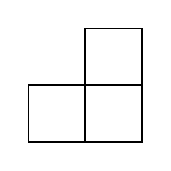
\begin{tikzpicture}[x=.72cm,y=.72cm,line width=.65pt]
\draw (0,0) -- (2,0) -- (2,2) -- (1,2) -- (1,1) -- (0,1) -- cycle;
\draw (1,0) -- (1,1) -- (2,1);
\end{tikzpicture}}\endgroup\par
Three faces unfolded into the plane, with no labels.}
\end{GelfandAdjacentEvidence}
\begin{GelfandAdjacentEvidence}{GELFAND-P000627}{5}

[To the right of the figure:] go round a closed path in the plane
corresp. path on the cube: we will arrive at another point (torsion)
and turn (curvature).

It is unclear what the basic geom. things look like on polyhedra (\(n\)-dimensional case).
Char. classes and so on. [crossed out]
\Incomplete{GELFAND-P000627}{cancelled-geometry}{A short entry after “and so on” is heavily crossed out.}
\end{GelfandAdjacentEvidence}
\begin{GelfandAdjacentEvidence}{GELFAND-P000627}{6}

\underline{Problem:} make a general theory of relativity on lattices.

\underline{A list of what one needs to know from physics (for a sensible mathematician).}

1. Feynman, Hibbs «Quant. Mech. and Path Ints.».

2. Feynman’s lectures for schoolchildren.

3. Quantum mechanics: Landau, Lifshitz (perturbation theory, quasiclassical approximation
[crossed out], Lie groups, basic concepts of scattering theory).
\Unclear{GELFAND-P000627}{landau-short}{A sign resembling a parenthesis is crossed out after “approximation”. A comma is visible to its right.}
\end{GelfandAdjacentEvidence}
\begin{GelfandAdjacentEvidence}{GELFAND-P000627}{7}


4. Relativ. quant. mech. --- the beginning of Berestetskii, Lifshitz, Pitaevskii; second quantization
(Dirac’s book [crossed out]; Feynman «Stat. Mechanics»).
\Unclear{GELFAND-P000627}{dirac-short}{A sign resembling a parenthesis is crossed out after “Dirac”. A semicolon is visible to its right.}
\end{GelfandAdjacentEvidence}


Stat. physics --- Landau and Lifshitz.


\Needspace{7\baselineskip}
\begin{GelfandAdjacentEvidence}{GELFAND-P000628}{1}
\SourcePage{GELFAND-P000628}{unlabelled}
\underline{What mathematics should physicists know?}

1. Group reprs.

2. Pseudodiff. operators.

3. Fourier--Hörmander integral oper..

4. \(P^\lambda\) (Bernstein polynomials).
\[
LP^\lambda=a(\lambda)P^{\lambda-1}.
\]
\Unclear{GELFAND-P000628}{bernstein-coefficient}{The coefficient on the right reads \(a(\lambda)\).}
\end{GelfandAdjacentEvidence}
\begin{GelfandAdjacentEvidence}{GELFAND-P000628}{2}


5. Riemann--Roch theorem.

6. Relation of sing. to top. cycles.

\underline{Polyakov.}
\Incomplete{GELFAND-P000628}{cancelled-heading}{There is a heavily hatched strip below the surname.}
\end{GelfandAdjacentEvidence}
\begin{GelfandAdjacentEvidence}{GELFAND-P000628}{3}

[Right:] \underline{TMF, the next-to-last issue}; art. on the Yang--Mills field --- worked out in detail.

Yang, Mills --- trans. in the coll. «Elem. Particles and Compensating Fields» (1964).
\Unclear{GELFAND-P000628}{yang-citation}{The abbreviation before “в сб.” (in the collection) reads “перев.” (translation).}
\end{GelfandAdjacentEvidence}
\begin{GelfandAdjacentEvidence}{GELFAND-P000628}{4}


There are quarks \(q\simeq\begin{pmatrix}u\\d\\s\end{pmatrix}\).
quark spin \(\tfrac12\),
\(B\sim\) spin \(\tfrac12\) (baryon),
\(M\) --- spin \(0\) (meson).
\[
\begin{aligned}
M&\sim\overline q q&&\text{(quark and antiquark)},\\
B&\sim qqq.
\end{aligned}
\]
\underline{Where from}: Grouping into multiplets (8 at a time).
(the idea of Gell-Mann and Ne’eman).
\Unclear{GELFAND-P000628}{multiplets-word}{The entry reads “мультиплеты” (multiplets).}
\end{GelfandAdjacentEvidence}
\begin{GelfandAdjacentEvidence}{GELFAND-P000628}{5}

\Unclear{GELFAND-P000628}{neeman-name}{The second surname is written “Неймана”.}
\end{GelfandAdjacentEvidence}
\begin{GelfandAdjacentEvidence}{GELFAND-P000628}{6}

\(\Rightarrow\) Symmetries: the most suitable gr. \(SU(3)\),
reprs. \(\underline{8,10,27}\) (various).

\underline{Lowest representations?} [crossed out] scalar, stand., and tens. products.
\Unclear{GELFAND-P000628}{reps-short}{There is a short crossed-out mark before “scalar”.}
\end{GelfandAdjacentEvidence}
\begin{GelfandAdjacentEvidence}{GELFAND-P000628}{7}

Let these be real particles! remarkable idea:
\[
\begin{aligned}
3^*\times3&=1+8,\\
3\times3\times3&=1+8+8+10.
\end{aligned}
\]
\(\Rightarrow\) one cannot build mesons as 3 quarks; there are 8 of them, and \(3\times3=3^*+6\).

We scatter:
\[
\frac{\sigma(BB)}{\sigma(BM)}=\frac32
\qquad\text{(cross sections)}.
\]
--- that is how it comes out (accur. \(10\%\)).
High en. --- scattering of a [crossed out] particle on a particle as of a part. on an antiparticle.
\Incomplete{GELFAND-P000628}{scatter-cancelled-word}{A short word before “particle” is heavily crossed out.}
\end{GelfandAdjacentEvidence}
\begin{GelfandAdjacentEvidence}{GELFAND-P000628}{8}


\(\underline{qqqq\overline q}\) --- absent in experiment (called exotic).

Many particles --- speeds of rot. of quarks (like the electron in the hydrogen atom).
\underline{but}: unstable (resonance). Trans. to the ground state.
\Unclear{GELFAND-P000628}{rotational-abbrev}{The abbreviation before “вращ.” (rotation) reads “скор.”.}
\end{GelfandAdjacentEvidence}
\begin{GelfandAdjacentEvidence}{GELFAND-P000628}{9}


\underline{Baryon wave fn.:}
\[
\Delta^{++}\simeq u(x_1)u(x_2)u(x_3),
\]
but antisymm. is needed.

Propose 3 kinds and 3 colors.
\[
q=\begin{array}{@{}c@{\quad}l@{}}
\left(\begin{array}{ccc}
\makebox[12mm]{\(u_{\text{к}}\)}&\makebox[12mm]{\(u_{\text{ж}}\)}&\makebox[12mm]{\(u_{\text{с}}\)}\\
d_{\text{к}}&d_{\text{ж}}&d_{\text{с}}\\
s_{\text{к}}&s_{\text{ж}}&s_{\text{с}}
\end{array}\right)&
\begin{array}{@{}l@{}}
\text{up}\\
\text{down}\qquad\text{(Gell-Mann)}\\
\text{strange}
\end{array}\\[-1pt]
\begin{array}{ccc}
\makebox[12mm]{red}&\makebox[12mm]{yellow}&\makebox[12mm]{blue}
\end{array}&
\end{array}.
\]
\Unclear{GELFAND-P000628}{color-grid}{The matrix retains the source indices “к”, “ж”, “с”. The color names are written under the corresponding columns.}
\end{GelfandAdjacentEvidence}


In experiment quarks do not exist (\(90\%\)).
\(\mathcal L\) cannot be invar. under
\[
SU(3)\otimes SU_c(3)
\qquad\overset{\nwarrow}{\text{color (change of color)}}.
\]


\Needspace{7\baselineskip}
\begin{GelfandAdjacentEvidence}{GELFAND-P000629}{1}
\SourcePage{GELFAND-P000629}{unlabelled}
Assume that only colorless part. have masses that are not very large, colored ones --- \(\infty\).
\[
M\sim\overline q_{\text{к}}q_{\text{к}}+
\overline q_{\text{жс}}\overline q_{\text{жс}}+
\overline q_{\text{с}}q_{\text{с}}.
\]
\Unclear{GELFAND-P000629}{meson-index}{Both \(q\)s in the middle term are barred. Both subscripts tentatively read “жс”.}
\end{GelfandAdjacentEvidence}
\begin{GelfandAdjacentEvidence}{GELFAND-P000629}{2}

The Lagrangian must prohibit the appearance of colored particles (they must have inf. masses).
Let the interact. be carried by colored Yang--Mills fields (gluons).

\(SU(3)\) --- approx. symmetry. (\(20\)--\(30\%\)).
Let \(SU_c(3)\) --- be the exact group.
(Possibly there is a fourth kind (charmed), but there are certainly 3 colors).

Of mesons (see the fmla.) there should be 9. But there are more. Hence a fourth quark is necessary.
(4 years ago). [crossed out]\qquad \(SU(4)\otimes SU_c(3)\).
\Incomplete{GELFAND-P000629}{cancelled-quark-line}{The entry after “4 years ago” is heavily crossed out.}
\end{GelfandAdjacentEvidence}
\begin{GelfandAdjacentEvidence}{GELFAND-P000629}{3}

\[
\mathcal L=\overline q(i\gamma_\mu\nabla_\mu-m)q+
\frac{1}{4e^2}\operatorname{Sp}(F_{\mu\nu}^2).
\]
There are 8 Yang--Mills fields. (Gluons --- from glu --- glue --- stick quarks together).
They are massless. \underline{8 colored gluons}.

Conserved currents \(\Longleftrightarrow\) presence of symmetry.
We want to show that if the gr. is nonabelian \(\Rightarrow\)
\underline{interact. energy \(\sim\) [crossed out] \(R\)} (dist.)
(\(\Rightarrow\) the string joining the quarks does not break)
(in the abelian case \(\sim R^{-1}\), Maxwell eqs.).
\Unclear{GELFAND-P000629}{cancelled-potential}{A short entry with a horizontal stroke is crossed out before \(R\).}
\end{GelfandAdjacentEvidence}
\begin{GelfandAdjacentEvidence}{GELFAND-P000629}{4}

\[
\mathcal L=\frac{1}{4e^2}\operatorname{tr}(F_{\mu\nu}^2).
\]
\SourceFigure{GELFAND-P000629}{heavy-charges}{%
\par\smallskip
\begingroup\color{black}\GelfandFitDiagram{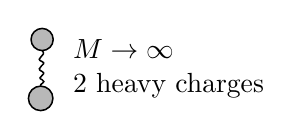
\begin{tikzpicture}[x=.74cm,y=.74cm,line width=.55pt]
\filldraw[fill=black!28] (0,1.57) circle (.19);
\filldraw[fill=black!28] (-.025,.56) circle (.21);
\draw (0,1.38) .. controls (.10,1.29) and (-.15,1.25) .. (0,1.19)
 .. controls (.11,1.15) and (-.15,1.08) .. (0,1.02)
 .. controls (.10,.97) and (-.12,.92) .. (0,.88)
 .. controls (.09,.83) and (-.06,.81) .. (-.025,.77);
\node[right,align=left] at (.36,1.07) {\(M\to\infty\)\\2 heavy charges};
\end{tikzpicture}}\endgroup\par
Two shaded circles are joined by a wavy line.}
\end{GelfandAdjacentEvidence}
\begin{GelfandAdjacentEvidence}{GELFAND-P000629}{5}


\underline{G. Classical vers.}: noncommut. electrical engineering.
\Unclear{GELFAND-P000629}{classical-heading}{The abbreviation after “Классич.” (classical) tentatively reads “вар.” (version).}
\end{GelfandAdjacentEvidence}
\begin{GelfandAdjacentEvidence}{GELFAND-P000629}{6}

\SourceFigure{GELFAND-P000629}{gluon-exchange}{%
\par\smallskip
\begingroup\color{black}\GelfandFitDiagram{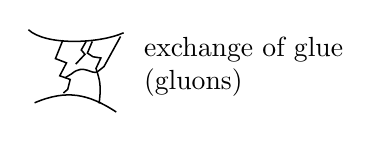
\begin{tikzpicture}[x=.78cm,y=.78cm,line width=.55pt]
\draw (0,1.2) .. controls (.28,.94) and (1.14,.97) .. (1.55,1.15);
\draw (.10,.01) .. controls (.62,.23) and (.97,.16) .. (1.43,-.14);
\draw (.56,1.03)--(.44,.73)--(.62,.66)--(.51,.45)--(.68,.39)--(.64,.23)--(.57,.17);
\draw (1.04,1.01)--(.96,.82)--(1.05,.76)--(1.18,.74)--(1.10,.57)
 .. controls (1.16,.38) and (1.19,.30) .. (1.15,.00);
\draw (1.50,1.09)--(1.23,.60)--(1.13,.52)
 .. controls (1.03,.45) and (.91,.66) .. (.70,.48)--(.60,.42);
\draw (.94,1.01)--(.86,.87)--(.92,.80)--(.77,.64);
\node[right,align=left] at (1.72,.60) {exchange of glue\\(gluons)};
\end{tikzpicture}}\endgroup\par
Two boundaries and connecting strokes. The exact joins in the middle are uncertain.}
\end{GelfandAdjacentEvidence}
\begin{GelfandAdjacentEvidence}{GELFAND-P000629}{7}

\SourceFigure{GELFAND-P000629}{pair-creation}{%
\par\smallskip
\begingroup\color{black}\GelfandFitDiagram{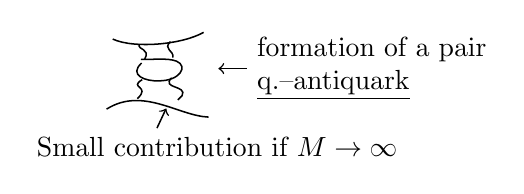
\begin{tikzpicture}[x=.78cm,y=.78cm,line width=.55pt]
\draw (0,1.16) .. controls (.35,1.00) and (1.13,1.07) .. (1.48,1.27);
\draw (-.10,.02) .. controls (.49,.39) and (1.07,-.09) .. (1.56,-.11);
\draw (.43,1.08) .. controls (.40,.97) and (.62,1.02) .. (.52,.83);
\draw (.94,1.12) .. controls (.81,.99) and (1.00,.98) .. (.98,.86);
\draw (.47,.77) .. controls (.25,.57) and (.54,.47) .. (.75,.48)
 .. controls (1.10,.48) and (1.23,.72) .. (1.04,.80)
 .. controls (.89,.86) and (.62,.82) .. (.46,.83);
\draw (.48,.50) .. controls (.25,.36) and (.63,.40) .. (.40,.19);
\draw (.96,.53) .. controls (.78,.35) and (1.22,.41) .. (1.13,.24)--(1.06,.17);
\draw[<-] (1.72,.68)--(2.19,.68);
\node[right,align=left] at (2.19,.68) {formation of a pair\\\underline{q.--antiquark}};
\draw[->] (.72,-.29)--(.87,.03);
\node[below,align=center] at (1.70,-.28) {Small contribution if \(M\to\infty\)};
\end{tikzpicture}}\endgroup\par
An oval between two boundaries. Arrows lead to the oval and to the lower line.}
\end{GelfandAdjacentEvidence}
\begin{GelfandAdjacentEvidence}{GELFAND-P000629}{8}

\Unclear{GELFAND-P000629}{heavy-note-word}{The first word beneath the sketch is overwritten and tentatively reads “Малый” (small).}
\end{GelfandAdjacentEvidence}
\begin{GelfandAdjacentEvidence}{GELFAND-P000629}{9}

\[
\begin{aligned}
\frac{\int DA_\mu\,e^{i\int\mathcal L\,d^4x}\,
          \operatorname{tr}e^{i\oint A_\mu\,dx_\mu}}
     {\int DA_\mu\,e^{i\int\mathcal L\,d^4x}}
&=\left\langle\operatorname{tr}e^{i\oint_C A_\mu\,dx_\mu}\right\rangle
=e^{iW(C)}.
\end{aligned}
\]
\Unclear{GELFAND-P000629}{action-dx}{The last character after \(d^4\) in the numerator is overwritten. It tentatively reads \(x\).}
\end{GelfandAdjacentEvidence}
\begin{GelfandAdjacentEvidence}{GELFAND-P000629}{10}

\Unclear{GELFAND-P000629}{line-integral-dx}{The \(x\) after \(d\) in the numerator contour integral is overwritten. No subscript \(C\) is visible on that integral.}
\end{GelfandAdjacentEvidence}
\begin{GelfandAdjacentEvidence}{GELFAND-P000629}{11}

\SourceFigure{GELFAND-P000629}{ordering-contour}{%
\par\smallskip
\begingroup\color{black}\GelfandFitDiagram{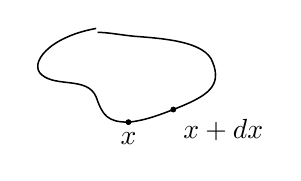
\begin{tikzpicture}[x=1cm,y=1cm,line width=.55pt]
\draw (.79,1.19) .. controls (.18,1.08) and (-.07,.74) .. (.10,.60)
 .. controls (.29,.44) and (.68,.58) .. (.79,.32)
 .. controls (.87,.09) and (.93,.00) .. (1.20,.00)
 .. controls (1.43,.02) and (1.67,.12) .. (1.87,.20)
 .. controls (2.20,.34) and (2.39,.46) .. (2.27,.76)
 .. controls (2.18,1.02) and (1.68,1.06) .. (1.28,1.09)
 .. controls (1.08,1.11) and (.94,1.14) .. (.81,1.14);
\fill (1.20,0) circle (.037) node[below] {\(x\)};
\fill (1.77,.16) circle (.037) node[below right] {\(x+dx\)};
\end{tikzpicture}}\endgroup\par
Two points are marked on the contour. A short stroke follows \(x+dx\). No index can be read with confidence.}
\end{GelfandAdjacentEvidence}
\begin{GelfandAdjacentEvidence}{GELFAND-P000629}{12}

\[
\operatorname{tr}\prod_x(1+iA_\mu(x)\,dx_\mu)
\]
--- contour integral. (this ordering).
(\(T\) --- Dyson exponential).

\underline{Assertion:}
\SourceFigure{GELFAND-P000629}{long-contour}{%
\par\smallskip
\begingroup\color{black}\GelfandFitDiagram{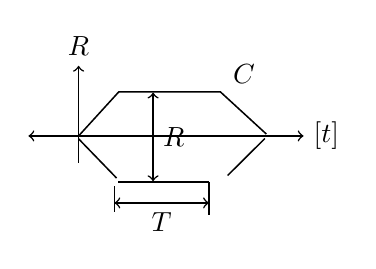
\begin{tikzpicture}[x=.91cm,y=.81cm,line width=.55pt]
\draw[<->] (-.70,0)--(3.14,0) node[right] {\([t]\)};
\draw[->] (0,-.42)--(0,1.10) node[above] {\(R\)};
\draw (0,0)--(.56,.69)--(1.98,.69)--(2.62,.03);
\draw (0,-.045)--(.53,-.66);
\draw (.55,-.72)--(1.82,-.72);
\draw (2.08,-.62)--(2.60,-.04);
\draw[<->] (1.04,-.71)--(1.04,.68) node[midway,right] {\(R\)};
\draw (.50,-.79)--(.50,-1.20);
\draw (1.82,-.72)--(1.82,-1.24);
\draw[<->] (.50,-1.05)--(1.82,-1.05) node[midway,below] {\(T\)};
\node[above] at (2.31,.67) {\(C\)};
\end{tikzpicture}}\endgroup\par
Contour \(C\), the \(R\) axis, and spans \(R\) and \(T\). There is a gap at the right of the lower side of the contour.}
\end{GelfandAdjacentEvidence}
\begin{GelfandAdjacentEvidence}{GELFAND-P000629}{13}

\Unclear{GELFAND-P000629}{graph-label}{The overwritten horizontal axis label tentatively reads \(t\).}
\end{GelfandAdjacentEvidence}

Consider such a contour.
Here \(W(C)\xrightarrow[T\to\infty]{}E(R)T\), where \(E(R)\)
--- the interaction energy of the charges.


\Needspace{7\baselineskip}
\begin{GelfandAdjacentEvidence}{GELFAND-P000630}{1}
\SourcePage{GELFAND-P000630}{unlabelled}
\underline{Explanation:} if the syst. is in a stat. state,
the trans. amplitude in time \(T\): \(F=e^{-iET}\) (\(E\) --- energy).
\Unclear{GELFAND-P000630}{stationary-phase}{The exponent is written \(-iET\). A separate stroke is visible above the first \(F\).}
\end{GelfandAdjacentEvidence}
\begin{GelfandAdjacentEvidence}{GELFAND-P000630}{2}

\underline{On the other hand}
\[
F=e^{-iET}=\sum_{(\text{paths})} e^{iS}.
\]
\SourceFigure{GELFAND-P000630}{time-path}{%
\par\smallskip
\begingroup\color{black}\GelfandFitDiagram{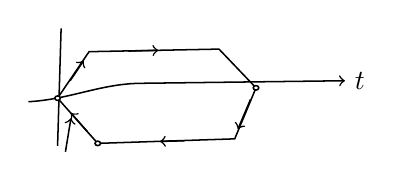
\begin{tikzpicture}[x=1cm,y=.82cm,line width=.55pt]
\draw (0,-.74)--(.045,1.08);
\draw[->] (-.37,-.055) .. controls (.15,-.02) and (.54,.22) .. (1.04,.23)
 -- (3.65,.27) node[right] {\(t\)};
\draw (0,0)--(.40,.72)--(2.05,.76)--(2.52,.16)--(2.25,-.63)
 --(.51,-.70)--cycle;
\draw[->] (.16,.27)--(.33,.58);
\draw[->] (.90,.73)--(1.28,.74);
\draw[->] (2.45,-.02)--(2.29,-.48);
\draw[->] (1.61,-.66)--(1.30,-.67);
\draw[->] (.38,-.52)--(.17,-.23);
\draw[->] (.10,-.83)--(.17,-.31);
\draw[fill=white] (0,0) circle (.035);
\draw[fill=white] (.51,-.70) circle (.035);
\draw[fill=white] (2.52,.16) circle (.035);
\end{tikzpicture}}\endgroup\par
Arrows point right on the upper side and left on the lower side. A separate arrow points up toward the start.}
\end{GelfandAdjacentEvidence}
\begin{GelfandAdjacentEvidence}{GELFAND-P000630}{3}

[Beneath the figure:] creation of a part.--antipart. pair (superheavy); we hold it for a long time.

Classical action \(S=\int_{(x)}^{(x')}A_\mu\,dx_\mu\). In the el.-magn. field.
Antipart. \(\sim\) a part. going backward in time.
Hence \(W(C)\sim S_C\) (area inside the contour). \(\sim RT\to E\sim R\).
It is calculated by the saddle-point method.
\Unclear{GELFAND-P000630}{saddle-word}{The last word is written “перевала” (saddle point).}
\end{GelfandAdjacentEvidence}
\begin{GelfandAdjacentEvidence}{GELFAND-P000630}{4}

\[
\int DA_\mu\, e^{i\int(\partial_\mu A_\nu-\partial_\nu A_\mu)^2}
 e^{i\oint A_\mu\,dx_\mu}
=e^{-\oint\!\oint dx\,dx'\,D(x-x')},
\]
where \(D=\dfrac{1}{(x-x')^2+i0}\) (Green’s fn. of the d’Alembert eq.).
\[
W=\mathrm{const}\cdot T+\frac{e^2T}{R}+\ldots
\]

\underline{Next time:}
\[
\frac{\int DA\,e^{\frac{1}{4e^2}\int F_{\mu\nu}^{2}}\,
\text{[crossed out]}\cdot\operatorname{tr}e^{\oint A_\mu\,dx_\mu}}{N}
\qquad\text{--- we will calculate}.
\]
\Unclear{GELFAND-P000630}{cancelled-exponent-atom}{A short sign is crossed out before the contour integral. The insertion below reads \(\cdot\operatorname{tr}e\).}
\end{GelfandAdjacentEvidence}
\begin{GelfandAdjacentEvidence}{GELFAND-P000630}{5}

non-Gaussian, since \(F_{\mu\nu}\) has the quadr. term \([A_\mu,A_\nu]\).
\[
F_{\mu\nu}=\partial_\mu A_\nu-\partial_\nu A_\mu+[A_\mu,A_\nu].
\]
(In the el.-magn. field the commutator is \(0\)).
El.-dyn. with a compact gauge group --- nonuniqueness of extremals already arises.
\underline{Quarks in Yang--Mills have yet to be worked out.}
\Unclear{GELFAND-P000630}{closing-word}{The last word reads “сделана”, with the feminine ending.}
\end{GelfandAdjacentEvidence}

\begin{center}\textemdash\,\textperiodcentered\,\textemdash\end{center}


\Needspace{7\baselineskip}
\begin{GelfandAdjacentEvidence}{GELFAND-P000631}{1}
\SourcePage{GELFAND-P000631}{unlabelled}
\underline{9/\(\overline{\underline{\mathrm{II}}}\)-76.}\qquad\underline{Gelfand Sem.}
\Unclear{GELFAND-P000631}{date-day}{The digit of the day is heavily overwritten and reads “9”.}
\end{GelfandAdjacentEvidence}
\begin{GelfandAdjacentEvidence}{GELFAND-P000631}{2}

\underline{Krichever.}
\underline{Zakharov--Shabat eqs.}
\Unclear{GELFAND-P000631}{heading-short}{The ending of the abbreviation “Ур-я” (eqs.) is heavily overwritten.}
\end{GelfandAdjacentEvidence}
\begin{GelfandAdjacentEvidence}{GELFAND-P000631}{3}

\begin{equation*}
\left[L_1-\frac{\partial}{\partial y},L_2-\frac{\partial}{\partial t}\right]=0,\tag{1}
\end{equation*}
\[
\begin{aligned}
L_1&=\sum_{i=0}^n u_i(x,y,t)\frac{\partial^i}{\partial x^i},\\
L_2&=\sum_{i=0}^m v_i(x,y,t)\frac{\partial^i}{\partial x^i},
\end{aligned}
\qquad
\left.\begin{array}{ll}u_n=1,&u_{n-1}\\v_m=1,&v_{m-1}\end{array}\right\}
=\mathrm{const}.
\]
\Incomplete{GELFAND-P000631}{coeff-cancelled-expression}{An entry after \(u_n\) is crossed out, with \(=1\) above it. A \(1\) is inserted below \(v_m\).}
\end{GelfandAdjacentEvidence}
\begin{GelfandAdjacentEvidence}{GELFAND-P000631}{4}


Consider the formal series
\begin{equation*}
\Psi=e^{kx+k^ny}\left(\sum_{i=0}^{\infty}\xi_i(x,y,t)\frac{1}{k^i}\right),
\qquad \xi_0=1.\tag{2}
\end{equation*}
Let \(\left(L-\dfrac{\partial}{\partial y}\right)\Psi=0\), where \(L=L_1\).
The coeffs. are computed recursively.
\begin{equation*}
\sum_{i=0}^n u_i\sum_{\ell=0}^i C_i^\ell\,\xi_{\ell-s}^{(i-\ell)}
=\xi_{n-s}+\frac{\partial}{\partial y}\xi_{-s},
\quad s=n,n-1,\ldots\ \text{down to }-\infty.\tag{3}
\end{equation*}
\(\xi_{-s}=0\) for \(s>0\).
\Unclear{GELFAND-P000631}{zero-index-range}{The sign before \(0\) is heavily overwritten. It tentatively reads \(>\).}
\end{GelfandAdjacentEvidence}
\begin{GelfandAdjacentEvidence}{GELFAND-P000631}{5}

[crossed out] determines \(\xi'_{n-s}\) \(\Rightarrow\) const. of integr. are needed.
\Incomplete{GELFAND-P000631}{cancelled-before-determined}{A short word before “determines” is crossed out.}
\end{GelfandAdjacentEvidence}
\begin{GelfandAdjacentEvidence}{GELFAND-P000631}{6}

\Unclear{GELFAND-P000631}{derivative-index}{The subscript of \(\xi'\) tentatively reads \(n-s\).}
\end{GelfandAdjacentEvidence}
\begin{GelfandAdjacentEvidence}{GELFAND-P000631}{7}

\(\xi_0=1,\quad \xi_i(0,y,t)=0\) for \(i>1\) --- normalization.
\Unclear{GELFAND-P000631}{normalization-bound}{The bound in the normalization is visibly written \(i>1\).}
\end{GelfandAdjacentEvidence}
\begin{GelfandAdjacentEvidence}{GELFAND-P000631}{8}

Conversely, \(\forall\) series \(\exists\) an oper., for which everything holds to accuracy \(k^{-1}\).

\underline{Algebraic operator.} --- if \(\exists\) an anal. continuation in \(1/k\)
to a compact alg. curve (merom. on the complement of the point, [below the line: where there is an essent. sing.]).

\underline{G.} Zakharov--Shabat eq.
\[
\frac{\partial K_2}{\partial y}-\frac{\partial K_1}{\partial t}=[K_1,K_2],
\]
\(K_1,K_2\) --- diff. operators.
\(K_1,K_2\) --- matr. in \(y\) and \(t\) or oper. in other variables.
There are many ways leading to this eq..
\(y,t\) --- parameters.
[Left: crossed out]
\Unclear{GELFAND-P000631}{margin-short}{The short crossed-out entry tentatively reads “На” (on).}
\end{GelfandAdjacentEvidence}

Put on an equal footing \(x,y,t\). Then it is written in the form (1).

Problem for schoolchildren: find oper. of the form
\[
-\frac{d^2}{dx^2}+u(x)=L_1,\qquad
\frac{d^3}{dx^3}+v_1\frac{d}{dx}+v_2=L_2,
\]
which commute. This is done via ellipt. fns. or ellipt. curves.
If we have only \(\dfrac{d^n}{dx^n}\), then
\[
\frac{d^n}{dx^n}\Psi-\frac{\partial\Psi}{\partial y}=0
\quad\Rightarrow\quad\Psi=e^{kx+k^ny}.
\]


\Needspace{7\baselineskip}
\begin{GelfandAdjacentEvidence}{GELFAND-P000632}{1}
\SourcePage{GELFAND-P000632}{unlabelled}
More precisely: the method of Fourier integral oper..
\[
e^{kx+k^ny}\left(1+\frac{\xi_1(x,y,t)}{k}+\ldots\right).
\]
\underline{Kr.} Associate to each oper. \(L\) --- the formal series (2).
The recurrence relation (3) recovers it uniquely up to normalization.

\underline{Definition.} \(L\) is called algebraic, if the formal series (2)
has a merom. continuation [inserted: (in the complement of the marked point)]
to a compact alg. curve, with poles independent of \(x,y,t\).
\Unclear{GELFAND-P000632}{marked-point-insertion}{“In the complement of the marked point” is inserted above the line.}
\end{GelfandAdjacentEvidence}
\begin{GelfandAdjacentEvidence}{GELFAND-P000632}{2}

\[
L\longrightarrow \text{[crossed out]}\ \mathcal R
\]
\Incomplete{GELFAND-P000632}{curve-cancelled-expression}{An entry after the arrow and before \(\mathcal R\) is heavily crossed out.}
\end{GelfandAdjacentEvidence}
\begin{GelfandAdjacentEvidence}{GELFAND-P000632}{3}

\(\mathcal R\) --- alg. curve with marked point \(P_0\) and set of poles
\(D_1+\ldots+D_g\), \(g\) --- genus of the curve
--- these are called scattering data for \(L\).
\Unclear{GELFAND-P000632}{polepoints-short}{The first sign after \(D_1\) is overwritten. It tentatively reads \(+\).}
\end{GelfandAdjacentEvidence}
\begin{GelfandAdjacentEvidence}{GELFAND-P000632}{4}

\(P_0\) --- point where there is an essent. sing..
\(1/k\) --- loc. param. near \(P_0\).

\underline{G.} An asympt. expansion as a rule does not converge.
The def. assumes convergence.
\underline{K.} To an alg. operator \(L\leadsto\) alg. curve with a marked point and a set of poles.
\underline{G.} \(C^\infty\) --- Taylor fmla. asympt. \(\Rightarrow\) analytic --- converg..
Analogue of quasianalyticity?

\underline{K.} \underline{Thm. (Akhiezer)}
\(\forall\) nonsing. alg. curve \(\mathcal R\) with marked point \(P_0\)
and a fixed loc. param. near \(P_0\) and a marked set of poles
\(\exists\) a fn. determined uniquely up to proportionality \(\Psi(x,y,P)\) with the given set of poles and
\[
\underbrace{\Psi(x,y,P)e^{-kx-k^ny}}_{1+o(1/k)}
\quad\text{--- reg. near }P_0.
\]
\Unclear{GELFAND-P000632}{little-o}{Below the bracket is \(1+o(1/k)\), with a small \(o\).}
\end{GelfandAdjacentEvidence}
\begin{GelfandAdjacentEvidence}{GELFAND-P000632}{5}

\SourceFigure{GELFAND-P000632}{rectangle-sketch}{%
\par\smallskip
\begingroup\color{black}\GelfandFitDiagram{\begin{tikzpicture}[x=1cm,y=1cm,line width=.55pt]
\draw (0,0) rectangle (1.55,1.08);
\end{tikzpicture}}\endgroup\par
Unlabelled rectangle.}
\end{GelfandAdjacentEvidence}
\begin{GelfandAdjacentEvidence}{GELFAND-P000632}{6}

\(e^{\zeta(P)x}\) [arrow to \(\zeta\):] Weierstrass (Kamke).

\underline{Proof:} explicit fmla. (will be presented later).
\underline{Thm.} The eq. is algebraic \(\Rightarrow\exists\) a fn. \(\Psi\)
\(\Rightarrow\) we know all the \(\xi\)
\(\Rightarrow\) we find all the \(u_i\) (uniquely) --- why do they exist?
From [crossed out] \(\Psi\) one finds the \(u_i\)!!
\Unclear{GELFAND-P000632}{bottom-short}{A short sign is crossed out before \(\Psi\).}
\end{GelfandAdjacentEvidence}
\begin{GelfandAdjacentEvidence}{GELFAND-P000632}{7}

[Lower right, crossed out: \(\forall\) series \(\exists\) an oper.:]
\Incomplete{GELFAND-P000632}{bottom-cancelled-insert}{A second short crossed-out entry stands beneath the left end of the cancelled line.}
\end{GelfandAdjacentEvidence}



\Needspace{7\baselineskip}
\begin{GelfandAdjacentEvidence}{GELFAND-P000633}{1}
\SourcePage{GELFAND-P000633}{unlabelled}
\(\forall\) series \(\exists\) an oper.:
\[
L\Psi-\frac{\partial}{\partial y}\Psi=
\text{[crossed out]}\left(e^{kx+k^ny}o(1/k)\right).
\]
(first \(n-2\) eqs.)
\Unclear{GELFAND-P000633}{series-word}{The first line reads “ряда” (series).}
\end{GelfandAdjacentEvidence}
\begin{GelfandAdjacentEvidence}{GELFAND-P000633}{2}

\Unclear{GELFAND-P000633}{top-cancel}{A short entry after the equals sign is heavily crossed out.}
\end{GelfandAdjacentEvidence}
\begin{GelfandAdjacentEvidence}{GELFAND-P000633}{3}

\Unclear{GELFAND-P000633}{top-o-argument}{The argument reads \(1/k\). The small round letter before it tentatively reads \(o\).}
\end{GelfandAdjacentEvidence}
\begin{GelfandAdjacentEvidence}{GELFAND-P000633}{4}


\(L\Psi-\dfrac{\partial\Psi}{\partial y}\)
meets all the requirements of Akhiezer’s thm. \(\Rightarrow\) it \(\equiv0\).

\underline{Drinfeld.}

\underline{An attempt at algebraizing Krichever’s previous talk}

Description of commut. subrings in the ring of diff. operators.

\underline{G.} The goal is a noncommut. reciprocity law.
\Unclear{GELFAND-P000633}{reciprocity}{The abbreviation before “law” reads “некомм.” (noncommutative).}
\end{GelfandAdjacentEvidence}
\begin{GelfandAdjacentEvidence}{GELFAND-P000633}{5}


\(B\) --- [crossed out] a comm. ring with \(1\), equipped with a deriv.
[crossed out] \(b\mapsto b'\) [crossed out].
(\(\mathbb C\)-algebra)
\Incomplete{GELFAND-P000633}{b-first-cancel}{The entry after \(B\) and the dash is heavily crossed out.}
\end{GelfandAdjacentEvidence}
\begin{GelfandAdjacentEvidence}{GELFAND-P000633}{6}

\Unclear{GELFAND-P000633}{b-derivative-cancel}{A short sign is crossed out after “дифф.” (deriv.).}
\end{GelfandAdjacentEvidence}
\begin{GelfandAdjacentEvidence}{GELFAND-P000633}{7}

\Unclear{GELFAND-P000633}{b-prime-cancel}{A short sign is crossed out after \(b'\).}
\end{GelfandAdjacentEvidence}
\begin{GelfandAdjacentEvidence}{GELFAND-P000633}{8}

\[
B[\mathcal D],\qquad
\underbrace{\sum b_i\mathcal D^i}_{\text{polyn.}},\qquad
\underbrace{Db-bD=b'}_{\text{multiplication rule}}.
\]
(\(b'\) --- derivative in \(B\))

\(X\) --- a compact Riem. surf. over \(\mathbb C\), \(P\) --- a fixed point.
Denote by \(A\) [crossed out] the ring of merom. fns. on \(X\) [crossed out]
with a pole only at \(P\).
\Unclear{GELFAND-P000633}{a-after-symbol}{A sign after \(A\) is heavily crossed out.}
\end{GelfandAdjacentEvidence}
\begin{GelfandAdjacentEvidence}{GELFAND-P000633}{9}

\Incomplete{GELFAND-P000633}{a-poles-cancel}{The word after \(X\) is heavily crossed out.}
\end{GelfandAdjacentEvidence}
\begin{GelfandAdjacentEvidence}{GELFAND-P000633}{10}


We describe the homomorphisms \(A\to B[\mathcal D]\).
(in fact there are no other comm. subrings --- Shabat’s thm.)

\underline{G.} The real problem: find all extensions of Gelfand--Kirillov skew fields.

Polynomiality gets in the way.
\[
\sum_{i=0}^{k} b_iD^i,\qquad
\underline{\text{ellipticity}}:\quad\exists b_k^{-1}.
\]
\underline{Req.}: the image of \(\forall\) nonzero elem. of \(A\) is elliptic.

\underline{Rank.} \(a\ne0,\quad a\in A\).
\[
\left.
\begin{gathered}
\operatorname{ord}(a)\text{ --- order of the image of }a\\
\operatorname{ord}(ab)=\operatorname{ord}(a)+\operatorname{ord}(b)\\
\operatorname{ord}(a+b)\le\text{[crossed out]}\max(\operatorname{ord}(a),\operatorname{ord}(b))\\
\operatorname{ord}\lambda=0\quad\text{for }\lambda\in\mathbb C
\end{gathered}
\right]\quad\underline{\text{valuation}}.
\]
\Unclear{GELFAND-P000633}{norm-cancel}{An entry after the inequality sign is crossed out. It tentatively reads \(\operatorname{ord}(a)+\operatorname{ord}(b)\).}
\end{GelfandAdjacentEvidence}

\(\operatorname{deg}a\) --- order of the pole of \(a\) at the point \(P\).

\underline{Then} \(\underline{\operatorname{ord}(a)=n\operatorname{deg}(a)}\).
(clear for polynomials)

\(n\) --- rank of the homomorphism.

\underline{Krichever} --- \(n=1\) (coprimality of the orders of the oper.).
\par\smallskip\noindent\textemdash\,\textperiodcentered\,\textemdash\par
\(M=B[\mathcal D]\), \(M\) has the structure of a \(B\)-module;
\(\varphi:A\to B[\mathcal D]\).


\Needspace{7\baselineskip}
\begin{GelfandAdjacentEvidence}{GELFAND-P000634}{1}
\SourcePage{GELFAND-P000634}{unlabelled}
\(M_n\) --- oper. of order \(\le n\).

[crossed out: This is a \(B\)-submodule.]
\Unclear{GELFAND-P000634}{top-cancel}{The cancelled line tentatively reads “This is a \(B\)-submodule”.}
\end{GelfandAdjacentEvidence}
\begin{GelfandAdjacentEvidence}{GELFAND-P000634}{2}


\(M\) --- this is an \(A\otimes B\)-module, i.e. an
\(A\)-module and \(B\)-module and mult. by
\(A\) and \(B\) commute.
\[
\begin{aligned}
bx&=bx \quad\text{(mult. on the left)},\\
ax&=x\varphi(a),\\
a\in A&\Rightarrow aM_i\subset M_{i+\operatorname{deg}a\cdot n}.
\end{aligned}
\]
\(\nabla:M\to M\) --- mult. on the left by \(D\).
\[
\nabla(x)=Dx.
\]
\(\nabla\) commutes with the action of \(A\), and \(\nabla b-b\nabla=b'\).

\underline{Conversely,} if there is an \(A\otimes B\)-mod. \(M\)
with a filtr. and all these relations, then \(\exists\) a homom. \(\varphi:A\to B[\mathcal D]\)
of rank \(n\).

We can forget \(\varphi\) and consider the problem of \(A\otimes B\)-modules.

\(\rightarrow\) Thus, \(M\) --- a module over \(A\otimes B\),
equipped [crossed out] with the filtration
\[
0=M_{-1}\subset M_0\subset M_1\subset M_2\subset\cdots
\]
\Incomplete{GELFAND-P000634}{filtration-cancel}{A short entry before “filtration” is crossed out.}
\end{GelfandAdjacentEvidence}
\begin{GelfandAdjacentEvidence}{GELFAND-P000634}{3}

[Under \(A\): merom. fns. on \(X\) with a single pole.
Under \(B\): a ring (\(\mathbb C\)-alg.) with deriv. \(b\mapsto b'\).]
and with the operator \(\nabla:M\to M\), such that

\noindent 1) \(\nabla a=a\nabla\).

\noindent 2) \(\nabla b-b\nabla=b'\).

\noindent 3) \(\nabla(M_i)\subset M_{i+1}\),
\(\nabla:M_i/M_{i-1}\overset{\sim}{\to} M_{i+1}/M_i\)
for \(i\geqslant0\).
\Unclear{GELFAND-P000634}{condition-three-bound}{A separate slanted stroke lies below \(>\). The bound reads \(i\geqslant0\).}
\end{GelfandAdjacentEvidence}
\begin{GelfandAdjacentEvidence}{GELFAND-P000634}{4}


\noindent 4) \(bM_i\subset M_i\), \(M_i/M_{i-1}\) [crossed out]
a free \(B\)-module with one generator.
\Unclear{GELFAND-P000634}{condition-four-cancel}{A sign resembling an arrow is crossed out before “free”.}
\end{GelfandAdjacentEvidence}
\begin{GelfandAdjacentEvidence}{GELFAND-P000634}{5}


\noindent 5) \(aM_i\subset M_{i+n\operatorname{deg}a}\),
\[
a:M_i/M_{i-1}\overset{\sim}{\to}
M_{i+n\operatorname{deg}a}/M_{i+n\operatorname{deg}a-1}
\qquad\text{for }i\geqslant0.
\]
\Unclear{GELFAND-P000634}{condition-five-bound}{Item 5 repeats the sign with a separate stroke. The bound reads \(i\geqslant0\).}
\end{GelfandAdjacentEvidence}


\(\sim\) the data of a sheaf over \(X\otimes B\) with certain filtrations.

\(\nabla\sim\) a connection with a sing. at \(\infty\).
\begin{center}\textemdash\,\textperiodcentered\,\textemdash\end{center}


\Needspace{7\baselineskip}
\begin{GelfandAdjacentEvidence}{GELFAND-P000635}{1}
\SourcePage{GELFAND-P000635}{unlabelled}
\underline{23/\(\overline{\underline{\mathrm{II}}}\)-76.}\qquad\underline{Gelfand Sem.}

\underline{S. P. Novikov} on the work of M. Brodsky. (Minsk)

\underline{Some cases of explicitly solvable problems unrelated to KdV}.

\underline{Problem of vibrations of an elastic sphere.}
\[
-\frac{d^2y}{dr^2}+
\left(\lambda^2f^2(r)-\frac{\ell(\ell+1)}{r^2}\right)y
=\lambda_{k,\ell}y.
\]
\Unclear{GELFAND-P000635}{elastic-equation}{The right-hand side is written \(\lambda_{k,\ell}y\). A minus sign precedes the fraction in parentheses.}
\end{GelfandAdjacentEvidence}
\begin{GelfandAdjacentEvidence}{GELFAND-P000635}{2}

Inverse problem --- recover the par. of the elastic medium from the set of frequencies \(\lambda_{k,\ell}\).
The problem is overdetermined. Find when it is solvable and how.

Let \(rf(r)=u(r)\) be a monotone fn..

Consider
\[
m(\tau)=\int_{H(\tau)}^1
\left(\tau^{-2}f^2(r)-\frac1{r^2}\right)^{1/2}dr
\qquad\text{(Bohr quant. rule)}.
\]
(\(H(\tau)\) --- a zero of the expression under the radical)

Consider
\[
\tau^*_{k\ell}=\frac{\sqrt{\ell(\ell+1)}}{\lambda_{k\ell}},\qquad
m_{k\ell}=\frac{k+\tfrac14+C}{\sqrt{\ell(\ell+1)}}.
\]
\(\tau^*(m_{k\ell})=\tau^*_{k\ell}\) establishes a one-to-one corresp.

\(m_{k\ell}\) are dense everywhere;
nec. cond. --- \(\tau_{k\ell}\) dense.

\[
(rf(r))^{-1}=\psi(\eta).\qquad \tau(m)\longleftrightarrow m(\tau)
\]
\Unclear{GELFAND-P000635}{tau-correspondence}{The arrow between the expressions has heavy strokes at both ends.}
\end{GelfandAdjacentEvidence}
\begin{GelfandAdjacentEvidence}{GELFAND-P000635}{3}

\[
\psi(\eta)=\exp\Bigl(2\int^{1}(\tau^2-\eta^2)^{-1/2}
\frac{d(\tau m(\tau))}{d\tau}\,d\tau
\]
\Unclear{GELFAND-P000635}{inverse-integral}{The upper limit of the integral is written 1. The lower limit and the closing parenthesis are not visible.}
\end{GelfandAdjacentEvidence}
\begin{GelfandAdjacentEvidence}{GELFAND-P000635}{4}

Large \(\ell\) --- quasiclassics.

\underline{Fuchs.} There is a triang. manifold.
\SourceFigure{GELFAND-P000635}{triangulation}{%
\par\smallskip
\begingroup\color{black}\GelfandFitDiagram{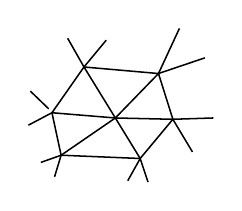
\begin{tikzpicture}[scale=.83,line width=.55pt]
\coordinate (a) at (-.91,.10);
\coordinate (b) at (-.42,.80);
\coordinate (c) at (.72,.70);
\coordinate (d) at (.94,.00);
\coordinate (e) at (.44,-.60);
\coordinate (f) at (-.77,-.55);
\coordinate (o) at (.06,.02);
\draw (a)--(b)--(c)--(d)--(e)--(f)--cycle;
\draw (-1.27,-.09)--(a)--(o)--(d)--(1.56,.02);
\draw (-.67,1.24)--(b)--(o)--(e)--(.56,-.96);
\draw (1.04,1.39)--(c)--(o)--(f)--(-.87,-.88);
\draw (b)--(-.08,1.21);
\draw (c)--(1.43,.94);
\draw (d)--(1.24,-.50);
\draw (e)--(.25,-.94);
\draw (f)--(-1.08,-.66);
\draw (-1.24,.43)--(-.96,.16);
\end{tikzpicture}}\endgroup\par
A triangular mesh with edges extending beyond it.}
\end{GelfandAdjacentEvidence}
\begin{GelfandAdjacentEvidence}{GELFAND-P000635}{5}

Consider \(\sum\) of all simplices of dim. 1 with coeff. \(1\bmod2\). It is not a cycle.

For the first barycentr. subdivision \(0\).
\SourceFigure{GELFAND-P000635}{barycentric}{%
\par\smallskip
\begingroup\color{black}\GelfandFitDiagram{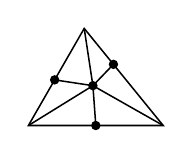
\begin{tikzpicture}[scale=.92,line width=.55pt]
\coordinate (a) at (-.91,0);
\coordinate (b) at (.95,0);
\coordinate (c) at (-.14,1.34);
\coordinate (d) at (-.5481,.6298);
\coordinate (e) at (.2633,.8442);
\coordinate (f) at (.02,0);
\coordinate (o) at (-.02,.55);
\draw (a)--(c)--(b)--cycle;
\draw (a)--(o)--(e) (b)--(o)--(d) (c)--(o)--(f);
\fill (d) circle (.065) (e) circle (.065) (f) circle (.065) (o) circle (.065);
\end{tikzpicture}}\endgroup\par
A triangle with three internal lines and four marked points.}
\end{GelfandAdjacentEvidence}
\begin{GelfandAdjacentEvidence}{GELFAND-P000635}{6}

\underline{all the centers}, \(\underline{0\bmod2}\) (even).

\underline{Stief. class --- is Poincaré dual to it}.
\Unclear{GELFAND-P000635}{stiefel-word}{The entry reads “Штиф. класс” (Stief. class).}
\end{GelfandAdjacentEvidence}

\[
\sum\text{ number }
\underset{\bmod 2}{=}
\sum(-1)^i\text{ of numbers }=\text{Euler char.}.
\]

\underline{Losik (Mark)}.

\underline{Connection.} \(E\to X\) vector bundle with fiber \(\mathbb R^n\);
\(p:P\to X\) assoc. principal bundle.

\(x\in X\), \(E_x\) --- fiber of \(E\) at \(x\).

\(P_x\ni z\), \(z=(e_{i,x})\), \(i=1,\ldots,n\),
\(z\) --- a basis in \(E_x\).

Consider \(G=GL(n,\mathbb R)\) and define its action on \(P\).
\[
A\in G\rightsquigarrow R_A:P\to P,\qquad
R_A(z)=zA=\left(\sum_{j=1}^{n}e_{j,x}A_i^j\right),
\quad A=(A_i^j),\quad i,j=1,\ldots,n.
\]
This action is smooth.


\Needspace{7\baselineskip}
\begin{GelfandAdjacentEvidence}{GELFAND-P000636}{1}
\SourcePage{GELFAND-P000636}{unlabelled}
\noindent 1. \((zA)B=z(AB)\).

\noindent 2. \(G\) preserves the fibers and acts simply transitively.

\(z\in P_x\), \(V_z\) --- vertical tangent space (\(\subset T_zP\)).
\(V_z=T_z(P_x)\).

define the map \(\ell_z:G\to P_x\), \(\ell_z(A)=zA\)

and the induced map \(\alpha_z:T_e(G)=\mathfrak g\to V_z\) (isomorphism).
\Unclear{GELFAND-P000636}{tangent-identification}{In \(T_e(G)=\mathfrak g\to V_z\), the lettering of \(\mathfrak g\) overlaps the strokes of the equals sign and arrow.}
\end{GelfandAdjacentEvidence}
\begin{GelfandAdjacentEvidence}{GELFAND-P000636}{2}


\(\beta_z=\alpha_z^{-1}:V_z\to\mathfrak g\)
(a linear form on \(V_z\) with values in \(\mathfrak g\)).

\underline{A connection on a principal bundle} --- a \(1\)-form on \(P\) with values in \(\mathfrak g\), such that

\noindent 1. \(\omega|_{V_z}=\beta_z\),

\noindent 2. \(R_A^*\omega=\operatorname{ad}A^{-1}\omega\) (invariance condition).

For the tangent bundle --- an affine connection.

Consider the equation \(\omega=0\) at the point \(z\),
\[
H_z=\{\xi\in T_zP:\omega(\xi)=0\}.
\]
\(H_z\) is called the horizontal space.
\(T_z=H_z\oplus V_z\).
\(H_z\) is preserved under the action of \(G\).

\begin{center}\textemdash\,\textperiodcentered\,\textemdash\end{center}

A bundle will be constructed whose sections are in one-to-one correspondence with connections on \(P\).

Consider \(T_z^*\otimes\mathfrak g\) --- \(1\)-forms at \(z\) with values in \(\mathfrak g\).

Define \(\Theta_z\subset T_z^*\otimes\mathfrak g\) as the subspace of those \(\Theta_z\), such that
\(\theta_z|_{V_z}=0\).
\Unclear{GELFAND-P000636}{theta-letter}{After “those”, the symbol resembles uppercase \(\Theta_z\). The restriction condition reads lowercase \(\theta_z\).}
\end{GelfandAdjacentEvidence}
\begin{GelfandAdjacentEvidence}{GELFAND-P000636}{3}


\[
\begin{aligned}
C_z&\subset T_z^*\otimes\mathfrak g,\qquad C_z\ni\omega_z:\omega_z|_{V_z}=\beta_z.\\
C_z-C_z&\subset\Theta_z,\qquad
\omega_{1,z}-\omega_{2,z}\in\Theta_z,\qquad
\omega_z+\Theta_z\in C_z.
\end{aligned}
\]
\Unclear{GELFAND-P000636}{affine-membership}{The last relation has the sign \(\in\) before \(C_z\).}
\end{GelfandAdjacentEvidence}


i.e. \(C_z\) --- a plane parallel to \(\Theta_z\), which does not pass through \(0\).

This gives a bundle of affine spaces
(«the difference of two Christoffel symbols is a tensor»).

Over \(P\) consider the bundle with fiber \(T_z^*\otimes\mathfrak g\).

There are maps:
\[
\widetilde r_{z,A}:T_z^*\otimes\mathfrak g\to T_{zA}^*\otimes\mathfrak g,
\]
induced by the maps
\(R_{A^{-1}}^*:T_z^*\to T_{zA}^*\) and
\(\operatorname{ad}A^{-1}:\mathfrak g\to\mathfrak g\).
[At right: Tensor product of maps.]


\Needspace{7\baselineskip}
\begin{GelfandAdjacentEvidence}{GELFAND-P000637}{1}
\SourcePage{GELFAND-P000637}{unlabelled}
\(C_z\) goes to the corresponding plane at \(zA\) under this map.

\[
C(P)=\bigcup_{z\in P}C_z
\]
--- a natural smooth bundle over \(P\).

\(G\) acts on \(C(P)\).

[Crossed out: \(C\)?] Invariant sections \(\longleftrightarrow\) connections.
\Unclear{GELFAND-P000637}{first-cancel}{The crossed-out entry before “Invariant” begins with a mark resembling \(C\).}
\end{GelfandAdjacentEvidence}
\begin{GelfandAdjacentEvidence}{GELFAND-P000637}{2}


\underline{\(C(P)/G=B(P)\)}, [“bundle” inserted and circled, with an arrow to \(\pi\)]
\(\pi:B(P)\to X\).
\Incomplete{GELFAND-P000637}{quotient-cancel}{The words below the circled “bundle” are heavily crossed out.}
\end{GelfandAdjacentEvidence}
\begin{GelfandAdjacentEvidence}{GELFAND-P000637}{3}


\(C(P)\) --- a principal bundle with base \(P\), there is a canonical connection there.

\underline{Gabrielov.}
[Crossed out: The connection \(\gamma\)? gives an isomorphism
\(T^*X\otimes\mathfrak g\to B(P)\).]
\Unclear{GELFAND-P000637}{gabrielov-symbol}{The cancelled symbol after “The connection” resembles \(\gamma\).}
\end{GelfandAdjacentEvidence}
\begin{GelfandAdjacentEvidence}{GELFAND-P000637}{4}


(on \(\forall\) fiber --- an affine transformation)

\(1\) conn. chosen \(\to\) another conn. determines a transformation of the original space.

(\(\Longleftrightarrow\) the difference of connections is a tensor)

\SourceFigure{GELFAND-P000637}{two-fiber-sketch}{%
\par\smallskip
\begingroup\color{black}\GelfandFitDiagram{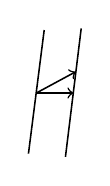
\begin{tikzpicture}[line width=.56pt]
\draw (-.23,0)--(-.03,1.57);
\draw (.24,-.04)--(.44,1.59);
\draw[->] (-.13,.77)--(.34,.77);
\draw[->] (-.13,.77)--(.37,1.04);
\end{tikzpicture}}\endgroup\par
Two slanted lines and two arrows pointing right in the margin.}
\end{GelfandAdjacentEvidence}


\par\noindent\begin{minipage}{\linewidth}
\[
\lambda\in T_xX\rightsquigarrow E_x\to E_x
\]
i.e. a form with values in homomorphisms.

\underline{\(T^*X\otimes\operatorname{Hom}(E,E)\)}.

\begin{center}\textemdash\,\textperiodcentered\,\textemdash\end{center}
\end{minipage}\par


\Needspace{7\baselineskip}
\begin{GelfandAdjacentEvidence}{GELFAND-P000638}{1}
\SourcePage{GELFAND-P000638}{unlabelled}
\underline{1/III-76.}\quad \underline{Gelfand Sem.}
\SourceFigure{GELFAND-P000638}{heading-ornament}{%
\par\smallskip
\begingroup\color{black}\GelfandFitDiagram{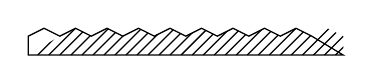
\begin{tikzpicture}[line width=.45pt]
\begin{scope}
\clip (0,0)--(4,0)--(4,.24)
  \foreach \x in {3.8,3.4,...,0.2} {--(\x,.34)--(\x-.2,.24)} --cycle;
\foreach \x in {-.3,-.16,...,4} {\draw (\x,0)--++(.34,.34);}
\end{scope}
\draw (0,.24) \foreach \x in {.2,.6,...,3.8} {--(\x,.34)--(\x+.2,.24)}
  --(4,0)--(0,0)--cycle;
\end{tikzpicture}}\endgroup\par
Hatched strip with a wavy upper edge below the heading.}
\end{GelfandAdjacentEvidence}
\begin{GelfandAdjacentEvidence}{GELFAND-P000638}{2}


\underline{Drinfeld.} (Volodya).

\(\overline X\) --- a smooth proj. curve over \(\mathbb C\),
\(P\) --- a fixed point on \(X\),

\(A\sim\) the ring of rat. fns. on \(X\) with a pole at \(P\)
(reg. on \(X\setminus P\)).
\Incomplete{GELFAND-P000638}{first-cancel}{A separate word below the definition of the ring is obscured by heavy hatching.}
\end{GelfandAdjacentEvidence}
\begin{GelfandAdjacentEvidence}{GELFAND-P000638}{3}


\underline{G. Example.} \(y^2=x(x-1)(x-2)\) (elliptic curve).
\[
P=\infty,\qquad A=\mathbb C[x,y]/(y^2-x(x-1)(x-2)).
\]
\Unclear{GELFAND-P000638}{field-overwrite}{The field symbol in the first quotient was overwritten. Tentatively \(\mathbb C\).}
\end{GelfandAdjacentEvidence}
\begin{GelfandAdjacentEvidence}{GELFAND-P000638}{4}


\underline{There is no fn. with a pole of order 1.} --- since
[crossed out] \underline{it is a torus}.
\Incomplete{GELFAND-P000638}{torus-cancel}{A short word between “since” and “it is a torus” is heavily crossed out.}
\end{GelfandAdjacentEvidence}
\begin{GelfandAdjacentEvidence}{GELFAND-P000638}{5}


doubly per.
\Unclear{GELFAND-P000638}{period-abbreviation}{The abbreviation reads “двоякопер.” (doubly periodic).}
\end{GelfandAdjacentEvidence}
\begin{GelfandAdjacentEvidence}{GELFAND-P000638}{6}

\SourceFigure{GELFAND-P000638}{torus-contour}{%
\par\smallskip
\begingroup\color{black}\GelfandFitDiagram{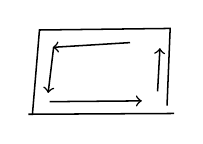
\begin{tikzpicture}[line width=.55pt]
\draw (0,0)--(.09,1.08)--(1.75,1.10)--(1.71,.12);
\draw (-.05,.01)--(1.80,.02);
\draw[->] (1.24,.92)--(.26,.86);
\draw[->] (.27,.86)--(.20,.28);
\draw[->] (.22,.17)--(1.39,.18);
\draw[->] (1.59,.30)--(1.62,.85);
\end{tikzpicture}}\endgroup\par
{\color{black}\(\underline{\int=0}\),\quad \underline{residue \(=0\)}.}\par\smallskip
Four arrows run counterclockwise along the contour.}
\end{GelfandAdjacentEvidence}
\begin{GelfandAdjacentEvidence}{GELFAND-P000638}{7}


Pole of order 2 --- Weierstrass \(\wp\)-fn.
(see Hurwitz, Courant).

[crossed out] \(y^2=x(x-1)\) of genus 0 --- \underline{Euler subst.}.
\Incomplete{GELFAND-P000638}{genus-zero-cancel}{A short word before the equation is heavily crossed out.}
\end{GelfandAdjacentEvidence}
\begin{GelfandAdjacentEvidence}{GELFAND-P000638}{8}


\(A\) for a curve of genus 0 --- polynomials, gen. \(z\).

\underline{\(A\) for an ell. curve} ---
\(\mathbb C[x,y]/(y^2-(x(x-1)(x-2))\).
\Unclear{GELFAND-P000638}{quotient-parenthesis}{The manuscript lacks a further closing parenthesis after the product.}
\end{GelfandAdjacentEvidence}


\(x\) has a pole of order 2. It goes to the Weierstrass fn. \(x=\wp(z)\),

\(y\) \textemdash\,\textquotedbl\,\textemdash\ order 3. \(y=\wp'(z)\).

The ring \(A\) uniquely determines the curve and the point.

How to describe these rings?

\begin{center}\textemdash\,\textperiodcentered\,\textemdash\end{center}

\underline{Krichever.}

almost \(\forall\) points \(P\) least pole order \(\underline{g+1}\).

\underline{Sometimes it can be lower} --- at Weierstrass points.

\[
y^2=\prod_{i=1}^{2g+1}(z-z_i)
\]
(hyperelliptic curve) --- at a branch point there is a fn. with a pole of order 2.

\(n\) --- least possible pole mult. at \(P\) \(\Rightarrow\) there are poles of mult. \(2n,3n,\ldots\).

Let \(\mu_s\) be such that \(\underline{\mu_s n+s}\) ---
pole multiplicity, \(s=1,\ldots,n-1\).

(\(\mu_s\) --- the least).

Then \(\underline{\mu_1+\cdots+\mu_{n-1}=g}\).
\quad \(\Vert\) all generators are among them. (Weierstrass theorem).


\Needspace{7\baselineskip}
\begin{GelfandAdjacentEvidence}{GELFAND-P000639}{1}
\SourcePage{GELFAND-P000639}{unlabelled}
\(P\) in general position --- the ring \(A\) has \(g\) generators ---
with poles of \(\underline{g+1,g+2,\ldots,2g+1}\) \underline{order}.
\Unclear{GELFAND-P000639}{generators-count}{The manuscript gives \(g\) before “generators” and lists orders from \(g+1\) to \(2g+1\).}
\end{GelfandAdjacentEvidence}
\begin{GelfandAdjacentEvidence}{GELFAND-P000639}{2}


\(B\) --- an algebra over \(\mathbb C\) with a derivation \(\mathcal D\).

There is a ring \(B[\mathcal D]=\{\sum b_iD^i\}\),
\(\mathcal Db-b\mathcal D=b'\).

An elem. is called elliptic if its lead. coeff. is invertible.

We describe homs. \(A\to B[\mathcal D]\), such that the image of \(\forall\) elem. is elliptic.

The rank of such a homomorphism is a (nat.) number \(n\), such that
\[
\forall a\in A,\quad \operatorname{ord}\varphi(a)=n\cdot\operatorname{deg}a.
\]
\(\operatorname{deg}a\) --- pole order of \(a\) [crossed out] at the point \(P\).
\Incomplete{GELFAND-P000639}{degree-cancel}{The entry after \(a\) is covered by heavy cross-out strokes.}
\end{GelfandAdjacentEvidence}
\begin{GelfandAdjacentEvidence}{GELFAND-P000639}{3}


(\underline{G.} There are diff. opers. of orders 2 and 3 that commute with each other.)

[crossed out: \(M\)?] homoms. \(\longleftrightarrow\) modules with additional structures.
\Unclear{GELFAND-P000639}{module-cancel}{The crossed-out mark resembles \(M\).}
\end{GelfandAdjacentEvidence}
\begin{GelfandAdjacentEvidence}{GELFAND-P000639}{4}


\underline{Krichever thm.}

The leading coefficient of the homomorphism \(\varphi:A\to B[\mathcal D]\).

Let \(z\) --- a local coordinate at \(P\).
Let \(a=z^{-k}+\cdots\) (Laurent).

[crossed out: Lead.?] \(\varphi(a)=b^k D^{nk}+\cdots\),
\Unclear{GELFAND-P000639}{leading-cancel}{The crossed-out entry tentatively reads “Стар” (lead.).}
\end{GelfandAdjacentEvidence}
\begin{GelfandAdjacentEvidence}{GELFAND-P000639}{5}


where \(\underset{\substack{\uparrow\\ B}}{b}\) is independent of \(k\)
and of the choice of loc. parameter.

(there are poles of \(\forall\) orders from a certain order onward. One has to divide)

\underline{\(b\) is called the leading coeff. of the homomorphism \(\varphi\)}.

\underline{def.} [crossed out: This is?] \(\varphi_1\sim\varphi_2\),
if \(\exists b\in B^*\),
\(\underline{\varphi_1(a)=b\varphi_2(a)b^{-1}}\).
\Unclear{GELFAND-P000639}{equivalence-cancel}{The crossed-out entry above the start of the definition tentatively reads “Это” (this is).}
\end{GelfandAdjacentEvidence}
\begin{GelfandAdjacentEvidence}{GELFAND-P000639}{6}


\(\dfrac{d}{dx}\sim\dfrac{b'}{b}+\dfrac{d}{dx}\).
Among germs, \(b'/b\) --- any fn..

\underline{Krichever thm.}
\(B\) [crossed out] --- germs of smooth fns. on the line.
\Incomplete{GELFAND-P000639}{germs-formula-cancel}{The formula after \(B\) is crossed out. Delimiters are visible, and the reading remains unresolved.}
\end{GelfandAdjacentEvidence}


homom. \(\varphi\) of rank \(1\) (up to equiv.!)
\(\longleftrightarrow\) the leading coeff. and a point on the Jacobian of the curve
(Jacobian variety), \(J_X\).

\underline{S. Gelf.}
\underline{1-dimensional vect. bundles of degree \(0\)}
(\(\sim\) divisor up to equivalence)
\[
\begin{array}{l@{\qquad}l}
Q_1,\ldots,Q_\ell & \\
n_1,\ldots,n_\ell & \text{degree } n_1+\cdots+n_\ell=0.\\
\multicolumn{1}{c}{\text{integers}} &
\end{array}
\]

\underline{equivalence}: if they differ by the divisor of a (meromorphic) fn..

\underline{Equiv.} --- bundles given by global merom. sections.


\Needspace{7\baselineskip}
\begin{GelfandAdjacentEvidence}{GELFAND-P000640}{1}
\SourcePage{GELFAND-P000640}{unlabelled}
\underline{G. Analytic def. of the Jacobian variety:} on \(\overline X\) there exist differentials of the first kind
(without sing.) there are \(g\) of them.

\(y^2=x(x-a)(x-b)\),

\(\Vert\dfrac{dx}{y}\) has no sing.
(at \(x=0,a,b\) there are none, since \(x\) is no loc. param.).

\SourceFigure{GELFAND-P000640}{abel-paths}{%
\par\smallskip
\begingroup\color{black}\GelfandFitDiagram{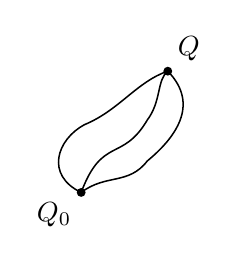
\begin{tikzpicture}[line width=.55pt]
\coordinate (q0) at (0,0);
\coordinate (q) at (1.10,1.54);
\draw (q0).. controls (-.46,.22) and (-.31,.67)..(.04,.86)
  .. controls (.48,1.04) and (.71,1.41)..(q);
\draw (q0).. controls (.27,.72) and (.52,.38)..(.84,.92)
  .. controls (1.02,1.16) and (.96,1.43)..(q);
\draw (q0).. controls (.32,.24) and (.60,.09)..(.84,.40)
  .. controls (1.18,.68) and (1.52,1.11)..(q);
\fill (q0) circle (1.6pt) node[below left] {\(Q_0\)};
\fill (q) circle (1.6pt) node[above right] {\(Q\)};
\end{tikzpicture}}\endgroup\par
Three paths between \(Q_0\) and \(Q\).}
\end{GelfandAdjacentEvidence}
\begin{GelfandAdjacentEvidence}{GELFAND-P000640}{2}


\(z_i=\int_{Q_0}^{Q}\omega_i\). [crossed out: This is?]
(\(\int\) over homol. classes. Basis --- \(g\) numbers)
\Unclear{GELFAND-P000640}{integral-cancel}{The crossed-out entry after the integral tentatively reads “Это” (this is).}
\end{GelfandAdjacentEvidence}
\begin{GelfandAdjacentEvidence}{GELFAND-P000640}{3}


the form determines a set of int. over periods.

up to periods --- \(\mathbb C^g/\underline{\text{lattice}}\).
\quad \(n_1\alpha_1+\cdots+n_{2g}\alpha_{2g}\).

Only some tori arise.

A divisor is a lin. comb. of points. Points of the torus can be added.

\SourceFigure{GELFAND-P000640}{divisor-motion}{%
\par\smallskip
\begingroup\color{black}\GelfandFitDiagram{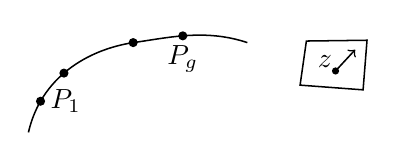
\begin{tikzpicture}[line width=.55pt]
\draw (0,0).. controls (.16,.70) and (.75,1.05)..(1.33,1.14)
  coordinate[pos=.21] (p1) coordinate[pos=.46] (p2) coordinate (p3)
  .. controls (1.77,1.20) and (2.24,1.32)..(2.78,1.14)
  coordinate[pos=.46] (pg);
\fill (p1) circle (1.65pt) node[right] {\(P_1\)};
\fill (p2) circle (1.65pt);
\fill (p3) circle (1.65pt);
\fill (pg) circle (1.65pt) node[below] {\(P_g\)};
\draw (3.45,.60)--(3.53,1.16)--(4.30,1.17)--(4.25,.54)--cycle;
\fill (3.90,.78) circle (1.3pt) node[above left,inner sep=1pt] {\(z\)};
\draw[->] (3.90,.78)--(4.15,1.05);
\end{tikzpicture}}\endgroup\par
Points on the curve and an arrow from \(z\) in a rectangle.}
\end{GelfandAdjacentEvidence}
\begin{GelfandAdjacentEvidence}{GELFAND-P000640}{4}


motion along a straight line on the torus \(\to\) motion of \(P_1,\ldots,P_g\) [crossed out] along the curve.
\Incomplete{GELFAND-P000640}{motion-cancel}{The word between \(P_g\) and “along the curve” is heavily crossed out.}
\end{GelfandAdjacentEvidence}
\begin{GelfandAdjacentEvidence}{GELFAND-P000640}{5}


\begin{center}\textemdash\,\textperiodcentered\,\textemdash\end{center}

Giving a hom. from \(A\) into the ring \(B[\mathcal D]\) is equiv. to giving the following.

\(M\) --- a module over \(A\otimes B\),
\(\nabla:M\to M\), \(\nabla(am)=a\nabla(m)\),
\(\nabla(bm)=b\nabla(m)+b'm\).

\[
0=M_{-1}\subset M_0\subset M_1\subset M_2\subset\cdots,\qquad
\dim_B M_i/M_{i+1}=1\quad\text{for }i\geqslant0.
\]
\Unclear{GELFAND-P000640}{reverse-quotient}{The manuscript writes \(M_i/M_{i+1}\) in the dimension statement.}
\end{GelfandAdjacentEvidence}
\begin{GelfandAdjacentEvidence}{GELFAND-P000640}{6}

\[
\begin{aligned}
BM_i&\subset M_i,\\
\nabla M_i&\subset M_{i+1},\qquad
\nabla_*:M_i/M_{i-1}\overset{\sim}{\to}M_{i+1}/M_i,\\
aM_i&\subset M_{i+\operatorname{deg}a},\\
a:M_i/M_{i-1}&\overset{\sim}{\to}M_{i+\operatorname{deg}a}/M_{i+\operatorname{deg}a-1}.
\end{aligned}
\]

\begin{center}\textemdash\end{center}

\underline{\(\varphi:A\to B[\mathcal D]\)}, \(\Rightarrow B[\mathcal D]=M\).
[crossed out: \(A\otimes B\)-module?]
\Unclear{GELFAND-P000640}{module-phrase-cancel}{The crossed-out line tentatively reads \(A\otimes B\)-module.}
\end{GelfandAdjacentEvidence}
\begin{GelfandAdjacentEvidence}{GELFAND-P000640}{7}


Mult. by \(B\) on the left and by \(A\) on the right,
\[
\begin{array}{rcl}
ma &=& m\varphi(a).\\[-.4ex]
   & \scriptstyle\mathrm{def} & \\[-.6ex]
bm &=& bm.
\end{array}
\]
\Unclear{GELFAND-P000640}{def-placement}{The mark \(\mathrm{def}\) is written between the two equals signs.}
\end{GelfandAdjacentEvidence}
\begin{GelfandAdjacentEvidence}{GELFAND-P000640}{8}


\(\nabla:M\to M\) mult. by \(\mathcal D\) on the left.

\underline{Filtr. --- order}.

\underline{last cond.} --- ellipticity.

\begin{center}\textemdash\,\textperiodcentered\,\textemdash\end{center}

How, from \(M\) to construct \(\varphi\)?

[crossed out: \(M\)?] \(M_{-1}=0\),
\Unclear{GELFAND-P000640}{m-cancel}{The crossed-out mark resembles \(M\).}
\end{GelfandAdjacentEvidence}
\begin{GelfandAdjacentEvidence}{GELFAND-P000640}{9}

\(\nabla:M_0\overset{\sim}{\to}M_1/M_0\).
in \(M_0\) there is a generator \(e\) (over \(B\)).

put \(D=\nabla(e)\).

\(\varphi(a)\) is clear since there is an \(A\)-module, etc..

\begin{center}\textemdash\,\textperiodcentered\,\textemdash\end{center}

\underline{Next step:} translate into the language of sheaves.

[crossed out: on the curve] \(M_{-1}=0\subset M_0\subset M_1\subset\cdots\)
\Unclear{GELFAND-P000640}{curve-cancel}{“On the curve” is crossed out before the filtration.}
\end{GelfandAdjacentEvidence}
\begin{GelfandAdjacentEvidence}{GELFAND-P000640}{10}


\(\sim\) a vect. bundle [inserted: 1-dimensional] on \(X\)
with \(0\) cohom. (0-dimensional and 1-dimensional) of the sheaf of sections.

[At right]
\[
aM_i\subset M_{i+\operatorname{deg}a},\qquad
a:M_i/M_{i-1}\overset{\sim}{\to}M_{i+\operatorname{deg}a-1}
\quad(i\geqslant0).
\]
\Unclear{GELFAND-P000640}{margin-graded}{Only one filtration term is written at the target of the arrow in the right margin.}
\end{GelfandAdjacentEvidence}



\Needspace{7\baselineskip}
\begin{GelfandAdjacentEvidence}{GELFAND-P000641}{1}
\SourcePage{GELFAND-P000641}{unlabelled}
\SourceFigure{GELFAND-P000641}{top-margin-mark}{%
\par\smallskip
\begingroup\color{black}\GelfandFitDiagram{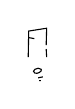
\begin{tikzpicture}[line width=.4pt,scale=.6]
\draw (0,.38)--(.01,.93)--(.39,.99)--(.38,.63) (.38,.55)--(.39,.38);
\draw (.02,.79)--(.13,.77);
\draw (.28,.12).. controls (.19,.19) and (.05,.08)..(.14,.04)
  .. controls (.20,.02) and (.29,.07)..(.28,.12);
\draw (.21,-.06)--(.31,-.04) (.23,-.12)--(.27,-.12);
\end{tikzpicture}}\endgroup\par
A three-sided mark at upper right with several detached strokes below.}
\end{GelfandAdjacentEvidence}
\begin{GelfandAdjacentEvidence}{GELFAND-P000641}{2}


\(L\) --- a 1-dimensional vect. bundle over \(\overline X\),
\(H^0(X,\underline L)=H^1(X,\underline L)=0\).

(\(H^0(X,\underline L)=0\) and \(\operatorname{deg}L=g-1\)).

\(M=H^0(X-P,\underline L)\) (algebraic sects.,
holom. with a single pole).
\Unclear{GELFAND-P000641}{holomorphic-abbrev}{The abbreviation after “algebraic sects.” reads “голом.” (holom.).}
\end{GelfandAdjacentEvidence}
\begin{GelfandAdjacentEvidence}{GELFAND-P000641}{3}


\(M_i\) [crossed out: \(-\)?] with a pole of order \(i+1\).
\Unclear{GELFAND-P000641}{m-i-cancel}{A short horizontal mark after \(M_i\) is crossed out.}
\end{GelfandAdjacentEvidence}
\begin{GelfandAdjacentEvidence}{GELFAND-P000641}{4}


\(M_{-1}=0\) --- first condition, (\(H^0=0\)).

\[
\dim M_i/M_{i-1}=1,\qquad
M_0=H^0(X,\underset{\substack{\uparrow\\\text{with a pole at }P}}{\underline L(P)}).
\]
\[
0\to\underline L\to\underline L(P)\to\underline L(P)/\underline L\to0.
\]
exact cohom. seq. \(\Rightarrow\dim_{\mathbb C}M_i/M_{i-1}=1\).

\begin{center}\shortstack{\textemdash\\[-.35em]\textemdash}\end{center}

Conversely, given a seq. of modules, construct a sheaf
\[
0=M_{-1}\subset M_0\subset M_1\subset M_2\subset\cdots,\qquad
\dim_{\mathbb C}M_i/M_{i-1}=1.
\]
\(M\) --- a module over \(A\).

\[
\begin{aligned}
aM_i&\subset M_{i+\operatorname{deg}a}\\
a_*:M_i/M_{i-1}&\overset{\sim}{\to}
M_{i+\operatorname{deg}a}/M_{i+\operatorname{deg}a-1},\qquad i\geqslant0.
\end{aligned}
\]
\Unclear{GELFAND-P000641}{graded-symbol}{The subscript on \(a\) in the map resembles an asterisk.}
\end{GelfandAdjacentEvidence}
\begin{GelfandAdjacentEvidence}{GELFAND-P000641}{5}


\underline{We give sects. of the sheaf on Zariski open sets}.

The sheaf is quasi-coherent. It suffices to give it on open affine subsets.

\(a_0\in A\), \(a_0\ne\mathrm{const}\) \(\Vert\) cover
\[
X=(X\setminus P)\cup(X\setminus\text{zeros of }a_0).
\]
Sects. over \(X\setminus P\), \(A\)-module --- \(M\).

Over \(X\setminus\text{zeros of }a_0\) --- \(m/a_0^k\),
\(m\in M_{k\cdot\operatorname{deg}a_0-1}\).

\underline{Next time:} Drinfeld \(20\) min., Shnirelman.
\Incomplete{GELFAND-P000641}{bottom-clipped}{Only isolated upper strokes are discernible below the last line.}
\end{GelfandAdjacentEvidence}



\Needspace{7\baselineskip}
\begin{GelfandAdjacentEvidence}{GELFAND-P000642}{1}
\SourcePage{GELFAND-P000642}{unlabelled}
\noindent\textperiodcentered\hfill\textemdash\,\textperiodcentered\,\textemdash\par
\underline{15/III-76 }\quad \underline{Gelfand Sem.}\quad \underline{Drinfeld.}

\(\overline X\) --- a smooth proj. curve over \(\mathbb C\)

\(P\in\overline X\),

\(A\in H^0(X-P,\mathcal O_X)\) --- rat. fns. on \(\overline X\) with a pole at \(P\).
\Unclear{GELFAND-P000642}{ring-membership}{The sign between \(A\) and \(H^0\) is \(\in\).}
\end{GelfandAdjacentEvidence}
\begin{GelfandAdjacentEvidence}{GELFAND-P000642}{2}


\(B\) --- an algebra over \(\mathbb C\) (with a deriv. [below: notation?]),
\(z\) --- a loc. coord. on \(\overline X\) near \(P\).
\Unclear{GELFAND-P000642}{derivation-insertion}{Below “with a deriv.” is an abbreviation resembling “обозн.” (notation), with two short strokes.}
\end{GelfandAdjacentEvidence}
\begin{GelfandAdjacentEvidence}{GELFAND-P000642}{3}


We seek homomorphisms \(\varphi:A\to B[\mathcal D]\) of rank \(1\),

i.e. \(\forall a\in A\), \(a=z^{-m}+\cdots\Rightarrow\varphi(a)=b^mD^m+\cdots\)

\(b\) --- the leading coefficient of \(\varphi\).

They are considered up to conjugation by inv. elements of \(B\).

[crossed out: \(B\)?] Giving \(\varphi\) is then equivalent to giving an
\(A\otimes B\)-module \(M\)
\Unclear{GELFAND-P000642}{assignment-cancel}{The mark crossed out before “Giving” resembles \(B\).}
\end{GelfandAdjacentEvidence}
\begin{GelfandAdjacentEvidence}{GELFAND-P000642}{4}


[crossed out: е?] and a map \(\nabla:M\to M\), such that
\Unclear{GELFAND-P000642}{first-cancel}{The short cancelled mark before “and a map” resembles “е”.}
\end{GelfandAdjacentEvidence}
\begin{GelfandAdjacentEvidence}{GELFAND-P000642}{5}


\(\nabla(am)=a\nabla(m)\), [crossed out: and?]
\(\nabla(bm)=b\nabla(m)+b'm\),
\(\underset{\text{(filtration)}}{M=\bigcup M_i}\),
\Unclear{GELFAND-P000642}{am-cancel}{The mark crossed out between the formulas for the map resembles “и” (and).}
\end{GelfandAdjacentEvidence}
\begin{GelfandAdjacentEvidence}{GELFAND-P000642}{6}


\(BM_i\subset M_i\), [crossed out: \(BM_i\)?]
\(M_{-1}=0\), \(M_i/M_{i-1}=B\) for \(i\geqslant0\).
\Unclear{GELFAND-P000642}{bm-cancel}{The crossed-out entry resembles \(BM_i\).}
\end{GelfandAdjacentEvidence}


\[
\begin{gathered}
\forall a\in A,\qquad aM_i\subset M_{i+\operatorname{deg}a},\\
a:M_i/M_{i-1}\overset{\sim}{\to}M_{i+\operatorname{deg}a}/M_{i+\operatorname{deg}a-1},\\
\nabla:M_i/M_{i-1}\overset{\sim}{\to}M_{i+1}/M_i,\qquad i\geqslant0.
\end{gathered}
\]

\underline{G. corollary:} \(\exists\) an oper. whose powers, except for the \(1\)st ---
are diff. operators (\(2\)nd, \(3\)rd etc.).

\(\overline X\) --- an alg. curve of genus \(g\), \(P\) --- a point.

\(n\) --- the least possible pole multiplicity at \(P\) (the sole pole).

\(\mu_i\) --- the least numbers for which there is a pole of mult. \(i+\mu_i n\), \(i=1,\ldots,n-1\).

Then \(\sum\mu_i=g\).


\Needspace{7\baselineskip}
\begin{GelfandAdjacentEvidence}{GELFAND-P000643}{1}
\SourcePage{GELFAND-P000643}{unlabelled}
[crossed out: There exist fn…?]
\Unclear{GELFAND-P000643}{cancel-top}{The crossed-out opening tentatively reads “Сущ. ф…” (there exist fn…).}
\end{GelfandAdjacentEvidence}
\begin{GelfandAdjacentEvidence}{GELFAND-P000643}{2}

(There are \(g\) omitted pole multiplicities\({}^*\))

[Arrow from the asterisk] this [crossed out] also conversely implies the statement formulated by Krichever.
\Incomplete{GELFAND-P000643}{cancel-top-right}{The word after “this” is heavily crossed out.}
\end{GelfandAdjacentEvidence}
\begin{GelfandAdjacentEvidence}{GELFAND-P000643}{3}


\underline{D. Into the language of sheaves.}

Everything except \(\nabla\), \(\sim\) specifying a vect. bundle \(L\) on \(\overline X\),
for which \(H^0(X,\underline L)=H^1(X,\underline L)=0\).

\(\sim\) specifying a 1-dimensional bundle \(L\) over \(X\otimes B\),
\[
H^0(X\otimes B,\underline L)=H^1(X\otimes B,\underline L)=0.
\]
\[
X=U_1\cup\cdots\cup U_k,\qquad U_i=\operatorname{Spec}R_i.
\]
Glue the aff. schemes \(\operatorname{Spec}\) [crossed out] \(R_i\otimes B\).
\Incomplete{GELFAND-P000643}{cancel-affine}{Marks between Spec and the expression on the right are heavily crossed out.}
\end{GelfandAdjacentEvidence}
\begin{GelfandAdjacentEvidence}{GELFAND-P000643}{4}


\underline{Intuitively:} a germ of a smooth family of vect. bundles.

\[
\nabla:\underline L\longrightarrow
\underset{\substack{\nearrow\\\text{with a first-order sing. at }P}}{\underline L(P)}
\qquad
\underline L\longrightarrow\underline L(P)/\underline L\longrightarrow0.
\]
[At right] \(H^0(\underline L(P)/\underline L)\) is free
(the restriction to \(P\) is trivial).

\(\nabla b-b\nabla=b'\), \(\nabla\) --- \(O_X\)-linear.

\underline{leading coeff.} --- ?

Trivialize near \(P\), Let \(e\) --- a basis.
\[
\frac{\nabla(e)}{e}=\frac{1}{b_0z}+\cdots
\quad\Rightarrow\quad b_0\text{ --- leading coeff.}.
\]

\underline{Krichever thm.}
Homom. of rank \(1\) up to conjugation by inv. elements of \(B\)
\(\Longleftrightarrow\) a point on the Jacobian of \(\overline X\) in general position.

\noindent 1. Given \(\varphi\). \(\Rightarrow\) a 1-dimensional bundle is given over \(X\otimes B\).
We construct a point on the Jacobian.

Let \(\mathbb C\leftarrow B\) and the corresp. embedding
\(\overline X\subset X\otimes B\), since there is a natural map \(B\to\mathbb C\)
(value at \(0\)).

Restrict \(L\) to \(\overline X\), i.e. obtain a vect. bundle on \(\overline X\).

\noindent 2. Let there be given \(L_0\) --- a bundle over \(\overline X\) and let there be given \(B\).
We construct everything else.

\(J\) --- the Jacobian of \(\overline X\), its points are vect. bundles of the same degree.

Tangent space to the Jacob. \(\cong H^1(X,O_X)\)
(the Jacobian itself \(H^1(X,O_X^*)\).
\(\Rightarrow\) the tangent space is obtained by removing \(*\)).

Consider the exact seq.
\[
0\longrightarrow O_X\longrightarrow O_X(P)
\longrightarrow O_X(P)/O_X\longrightarrow0.
\]
\Unclear{GELFAND-P000643}{sequence-overwrite}{The first letter of the third term has been overwritten. Tentatively \(O_X(P)/O_X\).}
\end{GelfandAdjacentEvidence}
\begin{GelfandAdjacentEvidence}{GELFAND-P000643}{5}

\Incomplete{GELFAND-P000643}{cancel-sequence}{A crossed-out entry is visible below the third term of the sequence.}
\end{GelfandAdjacentEvidence}
\begin{GelfandAdjacentEvidence}{GELFAND-P000643}{6}

[Upward arrow] a sheaf over a point.

Consider
\[
\frac{1}{[\text{crossed out}]z}\in H^0(O_X(P)/O_X)
\xrightarrow[\text{boundary hom.}]{} H^1(X,O_X).
\]
\Incomplete{GELFAND-P000643}{bottom-coefficient}{The mark before \(z\) in the denominator is obscured by ink.}
\end{GelfandAdjacentEvidence}

(\(z\) --- a loc. parameter).

The image of \(1/z\) in the tangent space to the Jacobian is denoted by \(\eta_P\in H^1(X,O_X)\).


\Needspace{7\baselineskip}
\begin{GelfandAdjacentEvidence}{GELFAND-P000644}{1}
\SourcePage{GELFAND-P000644}{unlabelled}
\(\ell_0\) --- the corresp. point on the Jacobian. As we vary \(x\) we get a smooth path on the Jacobian
(a point of the Jacobian with values in \(B\)).
\[
\underline{\ell'(x)=\frac{\eta_P}{b_0(x)}}
\]
(a straight line with changing parameter).
\Unclear{GELFAND-P000644}{top-point-letter}{The looped sign in both entries resembles \(\ell\) or \(e\).}
\end{GelfandAdjacentEvidence}
\begin{GelfandAdjacentEvidence}{GELFAND-P000644}{2}


\underline{Again:} curve \(X\), point \(P\), loc. param..

\(\Rightarrow\) a line in the tangent space to the Jacobian.

\(x\in\overline X\) [crossed out] \(x\mapsto\overline{x-P}\) --- \underline{divisor}.
\Incomplete{GELFAND-P000644}{cancel-divisor}{A group of looped signs is crossed out after the membership expression.}
\end{GelfandAdjacentEvidence}
\begin{GelfandAdjacentEvidence}{GELFAND-P000644}{3}


We obtain a map from \(\overline X\) into the Jacobian \(J\).

The curve has at \(P\) a tangent space.
The image --- a 1-dimensional space tangent to the Jacobian.

\begin{center}\textemdash\,\textperiodcentered\,\textemdash\end{center}

\underline{A. Polyakov.}\quad\underline{Gauge fields.}\quad\underline{Quantization of the Yang–Mills eqs.}

Lagrangian
\[
S=\int\mathcal L(x)d^4x,\qquad \mathcal L(x)=\frac14\operatorname{tr} F_{\mu\nu}^2.
\]
For the group \(\mathrm{SU}(2)\) we have \(F_{\mu\nu}\) --- an elem. of the Lie algebra.
\[
F_{\mu\nu}=\partial_\mu A_\nu-\partial_\nu A_\mu+g[A_\mu,A_\nu].
\]
[Outside the right rule]
\Unclear{GELFAND-P000644}{outer-edge-fragment}{The isolated mark resembles “э” or “3”.}
\end{GelfandAdjacentEvidence}
\begin{GelfandAdjacentEvidence}{GELFAND-P000644}{4}


\(A_\mu\), \(\mu=0,1,2,3\) --- anti-Hermitian with trace \(0\) (\(2\times2\)) (“traceless”).

The fields \(A_\mu\) --- dynamical variables.

Elem. fields --- fns. \(A_\mu(x)\), \(\mu=0,1,2,3\).
\[
A_\mu(x)\in\mathrm{SU}(2)\quad\text{(Lie alg.)}.
\]
\Unclear{GELFAND-P000644}{group-symbol}{The line reads \(SU(2)\), followed by “Lie alg.” in parentheses.}
\end{GelfandAdjacentEvidence}
\begin{GelfandAdjacentEvidence}{GELFAND-P000644}{5}

\[
F_{\mu\nu}^2=\sum_{\mu,\nu}F_{\mu\nu}F_{\mu\nu}.
\]
\Incomplete{GELFAND-P000644}{cancel-middle}{Several signs to the right of the sum are crossed out.}
\end{GelfandAdjacentEvidence}
\begin{GelfandAdjacentEvidence}{GELFAND-P000644}{6}


\(A_\mu\) is called the vect. potential,

\(F_{\mu\nu}\) \textemdash\,\textquotedbl\,\textemdash\ the field-strength tensor.

\underline{Passage to the Hamiltonian formalism.}\quad \(n=1,2,3\).
\[
L=\int\mathcal Ld^3\vec x=\operatorname{tr}\int
\left.\frac12(\dot A_n-\nabla_n A_0)^2-\frac12h_n^2\right\}d^3\vec x
\]
(we single out time)
\Unclear{GELFAND-P000644}{lagrangian-opening}{The manuscript has a closing brace. No opening brace is visible after the integral sign.}
\end{GelfandAdjacentEvidence}


Here \(\nabla_n A_0=\partial_n A_0+g[A_n,A_0]\)
(and we call it the covariant derivative).
\[
\begin{aligned}
h_n&=\frac12\varepsilon_{nm\ell}(\partial_m A_\ell-\partial_\ell A_m+g[A_m,A_\ell]),\\
F_{0n}&=\partial_0 A_n-\partial_n A_0+g[A_0,A_n].
\end{aligned}
\]
\[
\underline{\nabla_\mu X\underset{\mathrm{def}}{=}\partial_\mu X+g[A_\mu,X]}.
\]


\Needspace{7\baselineskip}
\begin{GelfandAdjacentEvidence}{GELFAND-P000645}{1}
\SourcePage{GELFAND-P000645}{unlabelled}
\(L\) does not contain \(\dot A_0\),
\(e_n=\dfrac{\partial\mathcal L}{\partial\dot A_n}=\dot A_n-\nabla_n A_0\)
--- \underline{canon. momentum}.

Hamiltonian.
\[
\underline{\mathcal H=e_n\dot A_n-\mathcal L}
=\frac12 e_n(e_n+\nabla_n A_0)+\frac12 h_n^2.
\]
\Unclear{GELFAND-P000645}{legendre-factor}{The manuscript has \(\tfrac12\) before \(e_n(e_n+\nabla_n A_0)\).}
\end{GelfandAdjacentEvidence}
\begin{GelfandAdjacentEvidence}{GELFAND-P000645}{2}

\[
H=\frac12\int d^3\vec x\,\operatorname{tr}[e_n^2+h_n^2-A_0\nabla_n e_n].
\]
\Unclear{GELFAND-P000645}{gauss-factor}{The prefactor of the integral reads one half.}
\end{GelfandAdjacentEvidence}
\begin{GelfandAdjacentEvidence}{GELFAND-P000645}{3}

\Unclear{GELFAND-P000645}{gauss-term}{A minus sign stands before \(A_0\nabla_n e_n\), with no separate numerical factor.}
\end{GelfandAdjacentEvidence}
\begin{GelfandAdjacentEvidence}{GELFAND-P000645}{4}

\[
-\frac{\delta H}{\delta A_0}=\dot e_0=0.
\]

Hamilton eqs. \(\leftrightarrow\) Lagrange eqs..

Hence let us impose the cond.
\[
\nabla_n e_n=0\tag{*}
\]
\[
\widehat H=\frac12\int d^3\vec x\,[e_n^2+h_n^2].
\]
\SourceFigure{GELFAND-P000645}{canonical-variables}{%
\par\smallskip
\begingroup\color{black}\GelfandFitDiagram{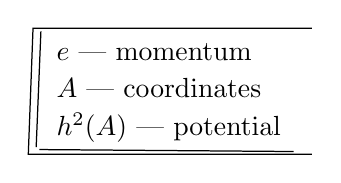
\begin{tikzpicture}[line width=.45pt]
\draw (3.6,1.6)--(.06,1.6)--(0,0)--(3.6,0);
\draw (.16,1.56)--(.10,.09) (.14,.06)--(3.37,.035);
\node[anchor=west,inner sep=2pt] at (.28,1.30) {\(e\) --- momentum};
\node[anchor=west,inner sep=2pt] at (.28,.84) {\(A\) --- coordinates};
\node[anchor=west,inner sep=2pt] at (.28,.34) {\(h^2(A)\) --- potential};
\end{tikzpicture}}\endgroup\par
A note in the right margin with an open-sided frame.}
\end{GelfandAdjacentEvidence}
\begin{GelfandAdjacentEvidence}{GELFAND-P000645}{5}


Will the cond. hold at the next instant \((*)\)?

Denote \(\nabla_n e_n=\rho(\vec x)\).

This is the condition \(\{\rho(x),H\}=0\), where
\[
\{A,B\}=\int d^3\vec x\sum_n
\left(\frac{\delta A}{\delta e_n}\cdot\frac{\delta B}{\delta A_n}
-\frac{\delta A}{\delta A_n}\frac{\delta B}{\delta e_n}\right).
\]
\[
\begin{cases}
\dot A_n=\dfrac{\delta H}{\delta e_n},\\
\dot e_n=-\dfrac{\delta H}{\delta A_n},\\
\nabla_n e_n=0.
\end{cases}
\]

[At right] \underline{These eqs. \(\sim\) the Lagrange eqs. This generalizes the usual result.}.

(generalization of Maxwell’s eqs. from \(U(1)\) to any [crossed out]
compact group --- and even a semisimple one).
\Incomplete{GELFAND-P000645}{cancel-group}{A word between “any” and “compact” is crossed out. Lower loops are visible.}
\end{GelfandAdjacentEvidence}
\begin{GelfandAdjacentEvidence}{GELFAND-P000645}{6}


\begin{center}\textemdash\,\textperiodcentered\,\textemdash\end{center}

\(\exists\) a comb. of Y.–M. fields on which the potential energy does not depend \(h^2\).
\[
\begin{aligned}
h_n&=\frac12\varepsilon_{nm\ell}F_{m\ell},\\
F_{m\ell}&=\partial_m A_\ell-\partial_\ell A_m+g[A_m,A_\ell].
\end{aligned}
\]
\[
\widetilde A_n(x)=\Omega^+A_n\Omega+\frac1g\Omega^+\partial_n\Omega(\vec x),
\]
\(\Omega(x)\) --- arbitrary matrix, \(\Omega(x)\in SU(2)\).

\(\underline{\widetilde h_n=\Omega^+h_n\Omega}\) --- \underline{checked directly}.

\(\Rightarrow\) the pot. en. [crossed out] invar.
(\(\operatorname{Sp}h^2\) does not change).
\Incomplete{GELFAND-P000645}{cancel-energy}{A short entry before “invar.” is heavily crossed out.}
\end{GelfandAdjacentEvidence}


Introduce the field \(a_n\). consider fields with cond. \(\underline{\partial_n a_n=0}\).

Set
\[
\begin{cases}
A_n(x)=\Omega^+(x)a_n\Omega(x)+\dfrac1g\Omega^+\partial_n\Omega(x),\\
\partial_n a_n=0.
\end{cases}
\]
[At right] \(\Vert\) a new set of variables.


\Needspace{7\baselineskip}
\begin{GelfandAdjacentEvidence}{GELFAND-P000646}{1}
\SourcePage{GELFAND-P000646}{unlabelled}
\underline{Canon. momentum split into two parts}.
\(P_n\), \(\rho(x)\), \(\partial_nP_n=0\).
\[
e_n=P_n+\partial_n\Psi,\qquad
H=\frac12\int(P_n^2+h_n^2(a)+(\partial_n\Psi)^2)d^3\vec x.
\]
To find \(\Psi\) we use that \(\nabla_n e_n\underset{\mathrm{def}}{=}\rho(\vec x)\).
\[
\begin{aligned}
\nabla_nP_n+\nabla_n\partial_n\Psi&=\rho,\\
\nabla_n\partial_n\Psi&=\rho+[P_n,a_n].
\end{aligned}
\]
\Unclear{GELFAND-P000646}{charge-commutator-first}{The first formula has \([P_n,a_n]\) with no factor \(g\).}
\end{GelfandAdjacentEvidence}
\begin{GelfandAdjacentEvidence}{GELFAND-P000646}{2}

\((\partial_n\Psi)^2\) is called \underline{Coulomb energy}.

\begin{center}\textemdash\,\textperiodcentered\,\textemdash\end{center}

\[
\begin{aligned}
H&=\int(e_n^2+h_n^2(A)),\\
A_n&\longrightarrow\Omega^+a_n\Omega+\Omega^+\partial_n\Omega,\\
\partial_n a_n&=0.
\end{aligned}
\]
\[
\begin{cases}
H=\int(P_n^2+(\partial_n\Psi)^2+h^2),\\
\nabla_n\partial_n\Psi=[a_n,P_n].
\end{cases}
\qquad\text{(Schwinger)}
\]
\Unclear{GELFAND-P000646}{schwinger-note}{The parenthesis at right reads “швингер” (Schwinger).}
\end{GelfandAdjacentEvidence}
\begin{GelfandAdjacentEvidence}{GELFAND-P000646}{3}

\Unclear{GELFAND-P000646}{charge-commutator-second}{Here the bracket reads \([a_n,P_n]\).}
\end{GelfandAdjacentEvidence}
\begin{GelfandAdjacentEvidence}{GELFAND-P000646}{4}


Here \(h_n(a)=\frac12\varepsilon_{nm\ell}(\partial_m a_\ell-\partial_\ell a_m+g[a_m,a_\ell])\).
\(\Psi\) is found from the last eq..

\[
\nabla_n e_n=\rho(\vec x)\quad\Rightarrow\quad
\left\{\begin{aligned}
\partial^2\Psi&=\rho(x)\quad\text{(in the scalar case)},\\
\int(\partial\Psi)^2dx&=\int\frac{\rho(x)\rho(y)}{|x-y|}\,dx\,dy.
\end{aligned}\right.
\]
--- Coulomb interaction.
\Unclear{GELFAND-P000646}{scalar-abbrev}{Above the equality the entry reads “в скал. случае” (in the scalar case).}
\end{GelfandAdjacentEvidence}
\begin{GelfandAdjacentEvidence}{GELFAND-P000646}{5}

\SourceFigure{GELFAND-P000646}{coulomb-callout}{%
\par\smallskip
\begingroup\color{black}\GelfandFitDiagram{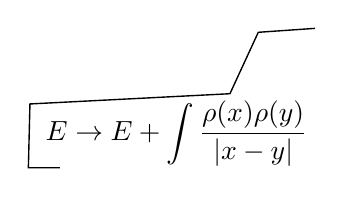
\begin{tikzpicture}[line width=.5pt]
\draw (.4,0)--(0,0)--(.02,.81)--(2.56,.94)--(2.92,1.72)--(3.64,1.77);
\node[anchor=west,inner sep=2pt] at (.14,.43)
  {\(\displaystyle E\to E+\int\frac{\rho(x)\rho(y)}{|x-y|}\)};
\end{tikzpicture}}\endgroup\par
A bent line connects the energy expression to the preceding formulas.}
\end{GelfandAdjacentEvidence}
\begin{GelfandAdjacentEvidence}{GELFAND-P000646}{6}


\underline{Non-Ab. case}. First by perturbation theory (first Khriplovich, then Gross, etc.).

\underline{Classical case:} \(g=0\Rightarrow\) the problem is Abelian.

We obtain
\[
\partial^2\Psi+g[a_n,\partial_n\Psi]=g[a_n,P_n]+\rho(x).
\]
\Unclear{GELFAND-P000646}{charge-commutator-last}{The right-hand side reads \(g[a_n,P_n]+\rho(x)\).}
\end{GelfandAdjacentEvidence}
\begin{GelfandAdjacentEvidence}{GELFAND-P000646}{7}


Approximations:
\[
\Psi^{(0)}=\frac1{\partial^2}\rho(x)
-\frac1{\partial^2}\left[a_n,\partial_n\frac1{\partial^2}\rho(x)\right].
\]
\Unclear{GELFAND-P000646}{perturbative-factor}{The second term has prefactor \(-1/\partial^2\). No separate factor \(g\) is visible.}
\end{GelfandAdjacentEvidence}
\begin{GelfandAdjacentEvidence}{GELFAND-P000646}{8}


\SourceFigure{GELFAND-P000646}{perturbation-graphs}{%
\par\smallskip
\begingroup\color{black}\GelfandFitDiagram{\begin{tikzpicture}[line width=.5pt]
\node[anchor=east,inner sep=1pt] at (0,0) {\(\Psi=\)};
\draw[dashed] (.12,0)--(1.23,0) (2.02,0)--(3.53,0) (4.28,0)--(5.79,0);
\node[below,inner sep=1pt] at (.12,0) {\(x\)};
\draw[->] (.62,.56)--(.52,.11);
\node[above,inner sep=1pt] at (.70,.52) {\(\scriptstyle 1/\partial^2\)};
\draw[->] (1.31,-.52)--(1.25,-.12);
\node[below,inner sep=1pt] at (1.34,-.51) {\(\scriptstyle\rho(y)\)};
\node at (1.62,0) {\(+\)};
\draw (2.76,.02)--(2.76,.45);
\node at (3.89,0) {\(+\)};
\draw (4.79,.02)--(4.79,.45) (5.12,.02)--(5.12,.45);
\foreach \x in {1.23,3.53,5.79} {
  \draw (\x-.055,-.055)--(\x+.055,.055) (\x-.055,.055)--(\x+.055,-.055);
}
\end{tikzpicture}}\endgroup\par
Three dashed diagrams with zero, one and two vertical branches.}
\end{GelfandAdjacentEvidence}
\begin{GelfandAdjacentEvidence}{GELFAND-P000646}{9}


[Below the first diagram]
\(\displaystyle\int\frac1{|x-y|}\rho(y)dy\).

Branch --- \(a_n\).

\SourceFigure{GELFAND-P000646}{one-branch-graph}{%
\par\smallskip
\begingroup\color{black}\GelfandFitDiagram{\begin{tikzpicture}[line width=.5pt]
\node[anchor=east,inner sep=2pt] at (0,0) {\(x\)};
\draw[dashed] (0,0)--(2.12,0);
\draw (.87,-.02)--(.87,.51);
\node[below,inner sep=2pt] at (.87,0) {\(z\)};
\draw (2.05,-.07)--(2.19,.07) (2.05,.07)--(2.19,-.07);
\node[below,inner sep=2pt] at (2.12,-.07) {\(y\)};
\end{tikzpicture}}\endgroup\par
The lower diagram has a branch at \(z\) and a cross above \(y\).}
\end{GelfandAdjacentEvidence}
\begin{GelfandAdjacentEvidence}{GELFAND-P000646}{10}

[At right]
\[
=\int\frac1{|x-z|}a_n(z)\frac{\vec\partial}{\partial z_n}
\frac1{|z-y|}\rho(y)\,d\vec y\,d\vec z.
\]
\Unclear{GELFAND-P000646}{kernel-derivative}{An arrow is written over the derivative sign in the numerator.}
\end{GelfandAdjacentEvidence}
\begin{GelfandAdjacentEvidence}{GELFAND-P000646}{11}


\[
\mathcal H\to\mathcal H+\int\rho(\bar x)
\underset{\substack{\Vert\\V}}{F(\bar x,\bar y,a)}
\rho(\bar y)\,d\bar x\,d\bar y.
\]
\Unclear{GELFAND-P000646}{kernel-mark}{Below the arguments of \(F\) are two short strokes and a sign resembling \(V\).}
\end{GelfandAdjacentEvidence}


Previously \(F=\dfrac1{|x-y|}\).
now \(F\) --- an operator.


\Needspace{7\baselineskip}
\begin{GelfandAdjacentEvidence}{GELFAND-P000647}{1}
\SourcePage{GELFAND-P000647}{unlabelled}
Passage to quant. mech. --- \(a,p\) --- opers.,
\(\left[a(x)\ p(y)\right]=\delta(x-y)\).
\Unclear{GELFAND-P000647}{canonical-bracket}{The second entry in the bracket reads \(p(y)\). The marks between entries are crowded, and a separate comma is indistinct.}
\end{GelfandAdjacentEvidence}
\begin{GelfandAdjacentEvidence}{GELFAND-P000647}{2}


\[
\delta E=\langle V\rangle=\int\rho(x)\langle F(x,y,a)\rangle\rho(y)\ldots
\]
(averaging)
\Unclear{GELFAND-P000647}{expectation-tail}{Three short strokes follow \(\rho(y)\). The integration measure is unwritten.}
\end{GelfandAdjacentEvidence}


\underline{5 April} --- \underline{continuation}.


\Needspace{7\baselineskip}
\begin{GelfandAdjacentEvidence}{GELFAND-P000648}{1}
\SourcePage{GELFAND-P000648}{unlabelled}
\underline{22/III-76.}\quad\underline{Gelfand Sem.}

\underline{G.}\quad\underline{A prob. distrib. arising from biology.}
\[
P_n=e^{-x_0-\alpha n}x_0\frac{(x_0+\alpha n)^{n-1}}{n!},
\qquad 0\leqslant\alpha<1.
\]
\Unclear{GELFAND-P000648}{probability-symbol}{The initial letter appears to be uppercase \(P\).}
\end{GelfandAdjacentEvidence}
\begin{GelfandAdjacentEvidence}{GELFAND-P000648}{2}


For \(\alpha=0\) --- Poisson distrib..

\underline{Exercise.} check that the sum equals \(1\).

“This is the only case where math. makes sense”. There is one more case in the literature.
\Unclear{GELFAND-P000648}{literature-phrase}{The end of the sentence reads “в лит-ре есть” (there is one in the literature).}
\end{GelfandAdjacentEvidence}
\begin{GelfandAdjacentEvidence}{GELFAND-P000648}{3}


\underline{Roiter.}

\(\Lambda\) --- a finite-dimensional algebra over the field \(k\).

There may be finitely or infinitely many indecomp. reps..

\underline{1968 Roiter}: if there are infinitely many, there are indecomp. reps. of arbitrarily large dimension.
\underline{Gabriel} --- a simpler proof.

(\underline{Maurice}) \underline{Auslander}:
1) generalized to Artinian rings.

\noindent 2) if \(\Lambda\) has infinitely many indecomp. reps., there are infinite chains of modules embedded in one another.
\[
A_1\to A_2\to A_3\to\ldots\to A_n\to\ldots
\]
\underline{Roiter reproved this with additional information}.
\Unclear{GELFAND-P000648}{reproved-abbrev}{The abbreviation before “with additional information” reads “передок.” (reproved).}
\end{GelfandAdjacentEvidence}
\begin{GelfandAdjacentEvidence}{GELFAND-P000648}{4}


\(\Lambda\) --- a finite-dimensional algebra, \(A\) --- an indecomp. module over \(\Lambda\).

\(\ell(A)\) --- length of the mod. \(A\) --- max. length
\[
0\subset A_1\subset A_2\subset\cdots\subset A_n=A.
\]
\(\bar\ell(A)\) --- max. length [inserted with arrow: of such a] chain of indecomp. modules.

\underline{We have} \(\ell(A)\geqslant\bar\ell(A)\).

\underline{Theorem} \(\forall\Lambda\) and \(\forall\) nat. \(N\), \(\exists n\):
\[
\bar\ell(A)\leqslant n\Longrightarrow\ell(A)\leqslant N.
\]
\Unclear{GELFAND-P000648}{length-quantifiers}{The arrow goes from \(\bar\ell(A)\leqslant n\) to \(\ell(A)\leqslant N\).}
\end{GelfandAdjacentEvidence}
\begin{GelfandAdjacentEvidence}{GELFAND-P000648}{5}


\begin{center}\textemdash\end{center}

There is an extended Dynkin diagram with \(n\) [crossed out] vertices.
\Incomplete{GELFAND-P000648}{cancel-vertices}{The word between \(n\) and “vertices” is heavily crossed out.}
\end{GelfandAdjacentEvidence}
\begin{GelfandAdjacentEvidence}{GELFAND-P000648}{6}

It has an associated quadr. form
\[
f(x_1,\ldots,x_n)=\sum_{i=1}^n a_i x_i^2+\cdots
\]
[At left] \underline{Kirillov.}

\underline{Dynkin diagram} one of the pictures.
\SourceFigure{GELFAND-P000648}{dynkin-drawings}{%
\par\smallskip
\begingroup\color{black}\GelfandFitDiagram{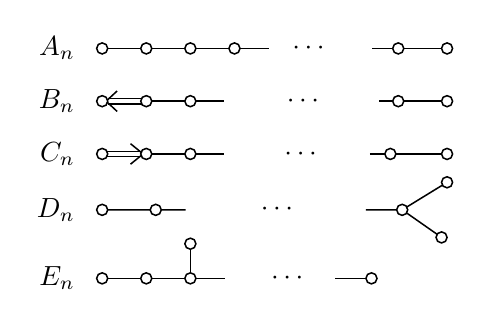
\begin{tikzpicture}[line width=.55pt,vertex/.style={circle,draw,fill=white,inner sep=0pt,minimum size=4pt}]
\node[anchor=east] at (-.22,0) {\(A_n\)};
\node[anchor=east] at (-.22,-.67) {\(B_n\)};
\node[anchor=east] at (-.22,-1.34) {\(C_n\)};
\node[anchor=east] at (-.22,-2.05) {\(D_n\)};
\node[anchor=east] at (-.22,-2.92) {\(E_n\)};
\draw (0,0)--(2.12,0) (3.43,0)--(4.38,0);
\draw (.56,-.67)--(1.55,-.67) (3.52,-.67)--(4.38,-.67);
\draw (.56,-1.34)--(1.55,-1.34) (3.40,-1.34)--(4.38,-1.34);
\draw (.08,-.637)--(.56,-.637) (.08,-.703)--(.56,-.703);
\draw (.19,-.54)--(.05,-.67)--(.19,-.80);
\draw (0,-1.307)--(.48,-1.307) (0,-1.373)--(.48,-1.373);
\draw (.36,-1.21)--(.52,-1.34)--(.36,-1.47);
\draw (0,-2.05)--(1.06,-2.05) (3.35,-2.05)--(3.81,-2.05)
  --(4.38,-1.70) (3.81,-2.05)--(4.31,-2.40);
\draw (0,-2.92)--(1.56,-2.92) (2.96,-2.92)--(3.42,-2.92) (1.12,-2.92)--(1.12,-2.48);
\node at (2.62,0) {\(\cdots\)};
\node at (2.55,-.67) {\(\cdots\)};
\node at (2.52,-1.34) {\(\cdots\)};
\node at (2.22,-2.05) {\(\cdots\)};
\node at (2.35,-2.92) {\(\cdots\)};
\foreach \x in {0,.56,1.12,1.68,3.76,4.38} {\node[vertex] at (\x,0) {};}
\foreach \x in {0,.56,1.12,3.76,4.38} {\node[vertex] at (\x,-.67) {};}
\foreach \x in {0,.56,1.12,3.66,4.38} {\node[vertex] at (\x,-1.34) {};}
\foreach \x in {0,.68,3.81} {\node[vertex] at (\x,-2.05) {};}
\node[vertex] at (4.38,-1.70) {};
\node[vertex] at (4.31,-2.40) {};
\foreach \x in {0,.56,1.12,3.42} {\node[vertex] at (\x,-2.92) {};}
\node[vertex] at (1.12,-2.48) {};
\end{tikzpicture}}\endgroup\par
Left column with the diagrams \(A_n,B_n,C_n,D_n,E_n\).}
\end{GelfandAdjacentEvidence}
\begin{GelfandAdjacentEvidence}{GELFAND-P000648}{7}


\SourceFigure{GELFAND-P000648}{dynkin-right}{%
\par\smallskip
\begingroup\color{black}\GelfandFitDiagram{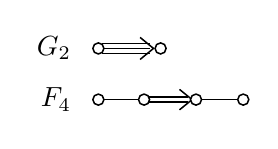
\begin{tikzpicture}[line width=.55pt,vertex/.style={circle,draw,fill=white,inner sep=0pt,minimum size=4pt}]
\node[anchor=east] at (-.22,0) {\(G_2\)};
\node[anchor=east] at (-.22,-.65) {\(F_4\)};
\foreach \y in {-.064,0,.064} {\draw (.04,\y)--(.65,\y);}
\draw (.53,.14)--(.70,0)--(.53,-.14);
\draw (0,-.65)--(.58,-.65) (1.24,-.65)--(1.84,-.65);
\draw (.58,-.617)--(1.14,-.617) (.58,-.683)--(1.14,-.683);
\draw (1.03,-.52)--(1.19,-.65)--(1.03,-.78);
\foreach \x in {0,.79} {\node[vertex] at (\x,0) {};}
\foreach \x in {0,.58,1.24,1.84} {\node[vertex] at (\x,-.65) {};}
\end{tikzpicture}}\endgroup\par
Right column with the diagrams \(G_2,F_4\).}
\end{GelfandAdjacentEvidence}
\begin{GelfandAdjacentEvidence}{GELFAND-P000648}{8}


[At right] and also for \(n=6,7,8\).

\begin{center}\(\longrightarrow\)\end{center}
[At left] \underline{Roiter.}

Dynkin diag. --- an integer-valued quadr. form
\[
\sum a_i x_i^2+\sum_{i<j}b_{ij}x_i x_j.
\]
additional conditions 1) positive definiteness.
\quad 2) \(a_i>0\).
\quad 3) \(b_{ij}\leqslant0\).
\quad 4) \(a_i\mid b_{ij}\) (divides).

[At right] \(\Vert\) one obtains precisely the Dynkin diagrams.

\SourceFigure{GELFAND-P000648}{valued-edge}{%
\par\smallskip
\begingroup\color{black}\GelfandFitDiagram{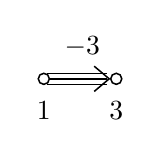
\begin{tikzpicture}[line width=.55pt,vertex/.style={circle,draw,fill=white,inner sep=0pt,minimum size=4pt}]
\foreach \y in {-.07,0,.07} {\draw (.04,\y)--(.80,\y);}
\draw (.64,.16)--(.83,0)--(.64,-.16);
\node[vertex] at (0,0) {};
\node[vertex] at (.92,0) {};
\node[below] at (0,-.16) {\(1\)};
\node[below] at (.92,-.16) {\(3\)};
\node[above] at (.49,.15) {\(-3\)};
\end{tikzpicture}}\endgroup\par
The lower diagram has \(1\) and \(3\) below the circles. The stroke before the upper \(3\) resembles a minus sign.}
\end{GelfandAdjacentEvidence}


\(\Vert\) \underline{Extended diag.} --- if the condition is replaced by nonnegative definiteness.


\Needspace{7\baselineskip}
\begin{GelfandAdjacentEvidence}{GELFAND-P000649}{1}
\SourcePage{GELFAND-P000649}{unlabelled}
A reflection is a change of one coord. of the vector that leaves the quadr. form unchanged. (lin. transf.).

Generate the group by all the refl.

Simple root --- \((0,0,\ldots,1,\ldots,0)\).

\underline{Root:} a vector obtained from a simple one by several reflections.

Given a vector \((x_1,\ldots,x_n)\). When is it a root?

If all the strokes are single, then root \(\Longleftrightarrow\) the quadr. form on it equals 1.
\Unclear{GELFAND-P000649}{single-strokes}{The abbreviation before “are single” reads “чёрт.” (strokes).}
\end{GelfandAdjacentEvidence}
\begin{GelfandAdjacentEvidence}{GELFAND-P000649}{2}


[Crossed out: If they are not all single] If they are not all single?
\Unclear{GELFAND-P000649}{cancel-not-all}{The first “If they are not all single” is crossed out with several strokes.}
\end{GelfandAdjacentEvidence}
\begin{GelfandAdjacentEvidence}{GELFAND-P000649}{3}


\underline{Thm.}
\[
(x_1,\ldots,x_n)\text{ --- root}\quad\Longleftrightarrow\quad
\forall i:\ f(x)\mid a_i x_i.
\]

\underline{Exercise} (for first-year students).
\[
\sum_{i=1}^{n} a_i x_i^2-\sum_{i<j}b_{ij}x_ix_j,
\qquad \frac{b_{ij}}{a_i}\in\mathbb{Z},\quad a_i>0.
\]

\SourceFigure{GELFAND-P000649}{star-drawing}{%
\par\smallskip
\begingroup\color{black}\GelfandFitDiagram{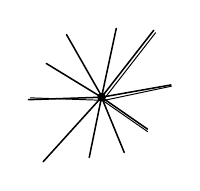
\begin{tikzpicture}[line cap=round,scale=.78]
\draw[line width=.55pt] (0,0)--(-1.19,-.04)
  (0,0)--(-.90,.55) (0,.02)--(-.57,1.02)
  (0,0)--(.24,1.12) (0,0)--(.85,1.09)
  (0,0)--(1.13,.20) (0,0)--(.75,-.52)
  (0,0)--(.37,-.90) (0,0)--(-.20,-.98) (0,0)--(-.95,-1.05);
\draw[line width=.35pt] (.04,-.03)--(.88,1.05)
  (.05,-.05)--(1.14,.18) (.03,-.06)--(.75,-.56)
  (.01,-.05)--(-1.16,-.01);
\fill (0,0) circle[radius=2pt];
\end{tikzpicture}}\endgroup\par
Rays at the left of the following formula. Some strokes are doubled.}
\end{GelfandAdjacentEvidence}
\begin{GelfandAdjacentEvidence}{GELFAND-P000649}{4}

\[
x_0^2+\cdots+x_n^2-x_0x_1-x_0x_2-\cdots-x_0x_n.
\quad \text{unclear.}
\]

Refl. --- a lin. transf. that leaves \(f(x)\) unchanged and changes only one coord.

[Crossed out: \(x\to\bar x\) and пр\ldots в., similar.]
\Incomplete{GELFAND-P000649}{cancel-description}{The interior letters of the crossed-out abbreviation are only partly legible.}
\end{GelfandAdjacentEvidence}

describe all the roots! (obtained by refl. from standard vectors) (\underline{ВОЛК}\(\to\)КОЗА).

[At right, column]
\begin{gather*}
\text{ВОЛК (wolf)}\\
\text{ПОЛК (regiment)}\\
\text{ПОЛА (coat flap)}\\
\text{ПОЗА (pose)}\\
\text{КОЗА (goat)}
\end{gather*}

\begin{center}\textemdash\enspace\textperiodcentered\enspace\textemdash\end{center}

\underline{Kirillov on Berezin’s talk.}
\[
x_i x_k=x_k x_i,\qquad x_1,\ldots,x_p
\]
\[
\xi_i\xi_k=-\xi_k\xi_i,\qquad \xi_1,\ldots,\xi_q
\]
\underline{Supermanifold:} Berezin, Leites.

[In the left margin] \underline{Following Rudakov.}

Consider the manifold \(M^p\) and the bundle \(E\to M^p\), whose fibre is a
\underline{Grassmann algebra} (with \(q\) generators)
(the struct. is specific to \(\forall\) point).

Morphisms are described in a more complicated way.

A fn. on a superman. is a smooth sect. of the bundle.

Integration rules. w.r.t. \(x\) as usual, and
\[
\int d\xi=0,\qquad \int\xi\,d\xi=1.
\]

Reps. of a 64-dimensional Lie superalgebra describe elem. particles better than reps. of \(SU(3)\).

Change of var.:
\[
\begin{cases}
x\to x+\xi_1\xi_2,\\
\xi_1\to\xi_1+x\xi_2,\\
\xi_2\to\xi_2+\xi_1\xi_2\xi_3
\end{cases}
\]
\[
\int P(\xi_1,\xi_2,\xi_3)\,d\xi_1\,d\xi_2\,d\xi_3
=\text{coeff. of the highest term.}
\]

\underline{Lie superalgebra:} \(\mathbb Z_2\)-graded, and
\[
[x,y]=-(-1)^{\deg x\cdot\deg y}[y,x].
\]

Jacobi id. \([x,\cdot]\) --- a homogeneous derivation.

\underline{more conv. def.:} a superalg. is obtained from a graded assoc. algebra by the rule
\[
[x;y]=xy-(-1)^{\deg x\cdot\deg y}yx.
\]

Lie thm. --- Berezin and Kac from Kyiv.

\begin{GelfandAdjacentEvidence}{GELFAND-P000649}{5}
\underline{G.’s remark.} \(p(t+\xi)=p(t)+p'(t)\xi\). Small quantities only of first order.
\Unclear{GELFAND-P000649}{first-order-phrase}{The first word tentatively reads “Малые” (small quantities).}
\end{GelfandAdjacentEvidence}



\Needspace{7\baselineskip}
\begin{GelfandAdjacentEvidence}{GELFAND-P000650}{1}
\SourcePage{GELFAND-P000650}{unlabelled}
Fns. on a superman. form a superalgebra.

There is a Poisson bracket.

Find deformations in the direction of the Poisson bracket.

\underline{Sinai.}\quad Theory of phase transitions --- spectra of matrices.

It was possible to calc. one of the interesting examples.
\Unclear{GELFAND-P000650}{sinai-examples}{The abbreviation after “of” tentatively reads “инт.” (interesting).}
\end{GelfandAdjacentEvidence}
\begin{GelfandAdjacentEvidence}{GELFAND-P000650}{2}


Dimension of the space \(2^n\).
\[
\begin{gathered}
a_{ij}\qquad a(\underbrace{x_1,\ldots,x_n}_{i},\underbrace{y_1,\ldots,y_n}_{j})\\
={e}^{\beta\left(J_1\sum_{i=1}^n x_i x_{i-1}
                  +J_2\sum_{i=1}^n x_i y_i\right)}.
\end{gathered}
\]
\(x_k=\pm1\), \underline{\(x_0=x_n\)}.
\Unclear{GELFAND-P000650}{spin-index}{The subscript on \(x\) is heavily overwritten and resembles \(k\).}
\end{GelfandAdjacentEvidence}
\begin{GelfandAdjacentEvidence}{GELFAND-P000650}{3}


\underline{Physical problem:} one needs to study \(\dfrac{e^{-\beta H}}{Z}\). Here [crossed out]
\Incomplete{GELFAND-P000650}{cancel-here}{A short passage after “Here” is heavily crossed out.}
\end{GelfandAdjacentEvidence}
\begin{GelfandAdjacentEvidence}{GELFAND-P000650}{4}

\[
\underline{\frac{\ln Z}{R^2}\underset{R\to\infty}{\longrightarrow}f(\beta).}
\]
The fns. \(f(\beta)\) can have singularities.

Study \(f(\beta)\) --- [crossed out]
\Incomplete{GELFAND-P000650}{cancel-study}{A short word before “there is” is heavily crossed out.}
\end{GelfandAdjacentEvidence}
\begin{GelfandAdjacentEvidence}{GELFAND-P000650}{5}

there is a transfer matrix (transfer-matrix).

Matrix with positive entries.
\SourceFigure{GELFAND-P000650}{lattice-diagram}{%
\par\smallskip
\begingroup\color{black}\GelfandFitDiagram{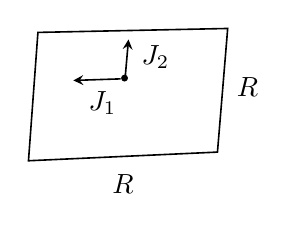
\begin{tikzpicture}[line width=.58pt,>=stealth]
\draw (0,0)--(2.40,.11)--(2.53,1.68)--(.12,1.63)--cycle;
\fill (1.22,1.05) circle[radius=1.25pt];
\draw[->] (1.17,1.04)--(.57,1.02);
\draw[->] (1.23,1.08)--(1.27,1.54);
\node[below] at (.94,1.01) {\(J_1\)};
\node[right] at (1.31,1.32) {\(J_2\)};
\node[right] at (2.52,.94) {\(R\)};
\node[below] at (1.20,-.05) {\(R\)};
\end{tikzpicture}}\endgroup\par
The arrows point left and up. The labels read as \(J_1\) and \(J_2\).}
\end{GelfandAdjacentEvidence}
\begin{GelfandAdjacentEvidence}{GELFAND-P000650}{6}

\[
Z=\sum e^{-\beta\sum_{x',x''}H(x',x'')},
\qquad \underline{Z=\operatorname{tr}A^R}.
\]
\Unclear{GELFAND-P000650}{trace-exponent}{The superscript is heavily overwritten and reads as \(R\).}
\end{GelfandAdjacentEvidence}

\(A^R\) --- transition matrix from layer to layer.

\underline{(Onsager’s 2-dimensional problem).}

\underline{Onsager computed all the eigenvalues of this matrix:}

Anticomm. variables help here: there are anticomm. matrices \(A_i,A_j\), such that
\[
A=e^{\sum c_{ij}A_i A_j}
\]
and the integrals can be calculated.

[In the right margin] \(\Vert\) see \underline{Huang} “\underline{Stat. Mech.}”.

\underline{Lieb} similarly calculated the entropy of square ice.

\begin{center}\textemdash\enspace\textperiodcentered\enspace\textemdash\end{center}


\Needspace{7\baselineskip}
\begin{GelfandAdjacentEvidence}{GELFAND-P000651}{1}
\SourcePage{GELFAND-P000651}{unlabelled}
\underline{29/III-76.}\quad \underline{Gelfand Sem.}

\underline{Krichever:}\quad \underline{problem:} solve the eq. \([L_1,L_2]=0\).
If \(\operatorname{ord}L_1\) and \(\operatorname{ord}L_2\) are coprime, the answer is a curve and a bundle
(1-dimensional).

The orders are not coprime --- multidimensional sheaves arise.

E.g. \underline{4th and 6th order --- not done}. Reduced to 2-dimensional bundles.
\[
\left.\begin{aligned}
L_1y&=E_1y\\
L_2y&=E_2y
\end{aligned}\right\}
\quad P(E_1,E_2)=0\quad\text{--- curve.}
\]
\Incomplete{GELFAND-P000651}{cancel-bundle}{A heavily crossed-out passage below the brace of the simultaneous equations.}
\end{GelfandAdjacentEvidence}
\begin{GelfandAdjacentEvidence}{GELFAND-P000651}{2}

Joint solution --- a 2-dimensional bundle over the curve.

Coprime --- the basis is 1-dimensional. (from the asymptotics).

\((m,n)=1\Longrightarrow\) the number of common eigenfns. equals \(n\). (and the eigenvalues are distinct)

\(E_1\) is determ. by \(E\); \(y\) a uniquely determ. fn. on a Riemann surf.
\Unclear{GELFAND-P000651}{eigenvalue-overwrite}{The subscript on the first \(E\) tentatively reads \(1\). The word “по” (by) is heavily overwritten.}
\end{GelfandAdjacentEvidence}
\begin{GelfandAdjacentEvidence}{GELFAND-P000651}{3}


\underline{Inverse problem:} construct commuting diff. ops. from the bundle --- not done.

\underline{Drinfeld.}
\[
d=(m,n)\Longrightarrow\quad
\text{specifying a pair of comm. ops.}\quad\Longleftrightarrow\quad
\text{specifying \((d-1)\) arbitrary fns.}
\]

\(B^{-1}LB\) can be solved --- 1 arbitrary fn. remains --- the leading coeff.

Orders 4 and 6 --- if square and cube --- already 2 arbitrary fns.

\underline{\underline{Shnirelman.}}\quad \(M\) --- an \(n\)-dimensional compact analytic Riemannian manifold,

\(\Delta\) --- Laplace op. on \(M\);
\[
\underline{\Delta u_k+\lambda_k^2u_k=0;}\qquad(1)
\]

\underline{def. of \(\Delta\):}
\SourceFigure{GELFAND-P000651}{sphere-sketch}{%
\par\smallskip
\begingroup\color{black}\GelfandFitDiagram{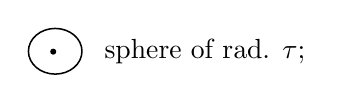
\begin{tikzpicture}[line width=.55pt]
\draw (0,0) ellipse[x radius=.34,y radius=.29];
\fill (-.025,-.005) circle[radius=1.1pt];
\node[right] at (.50,0) {sphere of rad. \(\tau\);};
\end{tikzpicture}}\endgroup\par
Circle with a dot at the centre.}
\end{GelfandAdjacentEvidence}
\begin{GelfandAdjacentEvidence}{GELFAND-P000651}{4}

\[
\frac{\text{avg. over sphere of rad. \(\tau\) --- value at centre}}{\tau^2}
\longrightarrow\Delta f(x).
\]

\underline{Growth as \(k\):}\quad \(\lambda_k\sim c k^{1/n}\), [crossed out: \(a\ldots\)]
\Incomplete{GELFAND-P000651}{cancel-square}{A sign resembling \(a\) is visible at the start of the cancellation.}
\end{GelfandAdjacentEvidence}
\begin{GelfandAdjacentEvidence}{GELFAND-P000651}{5}


Let \(a>0\). How is the following distributed \(\underline{a\cdot\lambda_k\bmod 2\pi}\)

(There are often arithmetic progressions).

\qquad --- subseq.

\underline{Torus.}
\SourceFigure{GELFAND-P000651}{torus-rectangle}{%
\par\smallskip
\begingroup\color{black}\GelfandFitDiagram{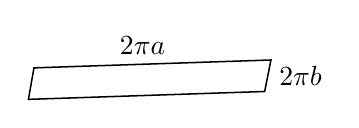
\begin{tikzpicture}[line width=.55pt]
\draw (0,0)--(3.0,.10)--(3.08,.50)--(.07,.40)--cycle;
\node[above] at (1.45,.44) {\(2\pi a\)};
\node[right] at (3.06,.30) {\(2\pi b\)};
\end{tikzpicture}}\endgroup\par
Rectangle under the heading “Torus”.}
\end{GelfandAdjacentEvidence}
\begin{GelfandAdjacentEvidence}{GELFAND-P000651}{6}

\[
\Delta u=\lambda^2u.
\]
\(\sin\alpha x\cdot\sin\beta y\)
[crossed out: \(\cos\ldots\)]
\Incomplete{GELFAND-P000651}{cancel-sine}{The start of the crossed-out entry resembles \(\cos\). The remaining signs are illegible.}
\end{GelfandAdjacentEvidence}
\begin{GelfandAdjacentEvidence}{GELFAND-P000651}{7}

or \(\cos\alpha x\cdot\sin\beta y\) etc.
\[
\lambda^2=\frac{n^2}{a^2}+\frac{m^2}{b^2},\qquad
\lambda=\sqrt{\frac{n^2}{a^2}+\frac{m^2}{b^2}}.
\]
Series --- for different \(n\) and \(m\) (for fixed).

Which 2 indices --- unclear.

\underline{Thm. for 1 dim.}
\Unclear{GELFAND-P000651}{first-dimension}{The last abbreviation tentatively reads “мер.” (dimension).}
\end{GelfandAdjacentEvidence}
\begin{GelfandAdjacentEvidence}{GELFAND-P000651}{8}

\[
-y''+u(x)y=\lambda y\quad\Longrightarrow\quad\text{on}
\]
\SourceFigure{GELFAND-P000651}{interval-sketch}{%
\par\smallskip
\begingroup\color{black}\GelfandFitDiagram{\begin{tikzpicture}[line width=.55pt]
\draw (0,0)--(1.45,0) (0,-.09)--(0,.09) (1.45,-.09)--(1.45,.09);
\end{tikzpicture}}\endgroup\par
Horizontal line with two end ticks.}
\end{GelfandAdjacentEvidence}
\begin{GelfandAdjacentEvidence}{GELFAND-P000651}{9}

\[
\sum_{i=0}^{n-1}c_i y_i\quad\text{has \(\leq n\) zeros}
\quad\Longrightarrow\quad\text{behaves like a polyn. of degree 1.}
\]

Hence 2 dim. --- a polynomial in \(n\) variables.
\Unclear{GELFAND-P000651}{second-dimension}{The abbreviation after 2 tentatively reads “мер.” (dimension).}
\end{GelfandAdjacentEvidence}
\begin{GelfandAdjacentEvidence}{GELFAND-P000651}{10}


\underline{Lowest --- positive everywhere.}

\underline{1st} --- like linear fns.

Next --- a curve of 2nd order.

follow the lin. combin.
\SourceFigure{GELFAND-P000651}{oval-chords}{%
\par\smallskip
\begingroup\color{black}\GelfandFitDiagram{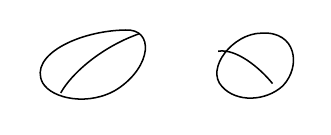
\begin{tikzpicture}[line width=.55pt]
\draw (-.85,0) .. controls (-1.03,.35) and (-.39,.66) .. (.20,.67)
 .. controls (.57,.69) and (.54,.21) .. (.10,-.08)
 .. controls (-.25,-.30) and (-.73,-.21) .. (-.85,0);
\draw (-.62,-.13) .. controls (-.49,.11) and (-.11,.45) .. (.37,.62);
\draw (1.43,-.05) .. controls (1.21,.18) and (1.57,.63) .. (1.93,.63)
 .. controls (2.37,.66) and (2.44,.21) .. (2.20,-.04)
 .. controls (1.98,-.24) and (1.61,-.25) .. (1.43,-.05);
\draw (1.38,.40) .. controls (1.60,.44) and (1.90,.20) .. (2.07,-.01);
\end{tikzpicture}}\endgroup\par
Two ovals. The sloping line in the left one runs from an interior point to the upper boundary. In the right one it runs from the left boundary to an interior point.}
\end{GelfandAdjacentEvidence}


\underline{\underline{Rayleigh}} --- theory of sound (2 volumes).

\underline{Arnold:} transfer Harnack’s thm. on the number of ovals (unknown for lin. combs.).

[In the right margin] \(\Vert\) For the \(n\)th eigenfn. the zeros divide the region \(\leq\) into \(n\) parts.


\Needspace{7\baselineskip}
\begin{GelfandAdjacentEvidence}{GELFAND-P000652}{1}
\SourcePage{GELFAND-P000652}{unlabelled}
Consider
\[
\Phi(\lambda,a)=\lim_{\varepsilon\to0}\varepsilon
\left(\sum\delta((\lambda-a\lambda_k)\bmod 2\pi)e^{-\varepsilon\lambda_k}
-\sum_k\frac{e^{-\varepsilon\lambda_k}}{2\pi}\right).
\]
\[
\mu_k=a\lambda_k\bmod 2\pi.
\]
\(\mu\) --- param. on the circle.
\Unclear{GELFAND-P000652}{distribution-letter}{The heavily retraced letter tentatively reads \(\mu\). The following words read “param. on the circle”.}
\end{GelfandAdjacentEvidence}
\begin{GelfandAdjacentEvidence}{GELFAND-P000652}{2}

\[
\Phi(\mu,a)=\lim_{\varepsilon\to0}\varepsilon
\left(\sum_{k=1}^{\infty}\delta(\mu-\mu_k)e^{-\varepsilon\lambda_k}
-\sum e^{-\varepsilon\lambda_k}/2\pi\right).
\]
[Arrow to the subtracted term] subtract so that the avg. value is \(0\). constant.

\(\Phi^\varepsilon(\mu,a)\) --- pre-limit expression.

\underline{Theorem.} Let \(\gamma_1,\gamma_2,\ldots\) --- closed geodesics on \(M\),
\(\ell(\gamma_1),\ell(\gamma_2),\ldots\) --- their lengths.
Let невд. расп.,
\Unclear{GELFAND-P000652}{nondegenerate-abbreviation}{The first Russian abbreviation resembles “невд.”. The next reads “расп.”.}
\end{GelfandAdjacentEvidence}
\begin{GelfandAdjacentEvidence}{GELFAND-P000652}{3}

in a discr. manner,
\Unclear{GELFAND-P000652}{dispersion-abbreviation}{The Russian abbreviation tentatively reads “дискр.” (discr.).}
\end{GelfandAdjacentEvidence}
\begin{GelfandAdjacentEvidence}{GELFAND-P000652}{4}

the lengths are all distinct and incommensurable. (general pos.).
\[
\Phi(\mu,a)\left\{
\begin{aligned}
&\equiv0&&\text{if } a\ne\frac pq\ell(\gamma_j),\\
&\not\equiv0&&\text{[crossed out] if } a=\frac pq\ell(\gamma_j).
\end{aligned}
\right.
\quad(p,q\in\mathbb Z)
\]
\Incomplete{GELFAND-P000652}{cancel-if}{The word before the second “if” is heavily crossed out.}
\end{GelfandAdjacentEvidence}
\begin{GelfandAdjacentEvidence}{GELFAND-P000652}{5}


[In the left margin]
\SourceFigure{GELFAND-P000652}{geodesic-loop}{%
\par\smallskip
\begingroup\color{black}\GelfandFitDiagram{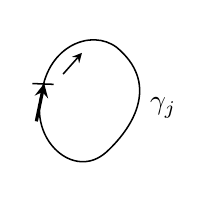
\begin{tikzpicture}[line width=.55pt,>=stealth]
\draw (-.57,.06) .. controls (-.49,.66) and (.06,.88) .. (.38,.64)
 .. controls (.91,.20) and (.63,-.34) .. (.25,-.69)
 .. controls (-.16,-1.06) and (-.74,-.53) .. (-.57,.06);
\draw[line width=1.15pt,->] (-.64,-.30)--(-.54,.18);
\draw (-.69,.18)--(-.42,.17);
\draw[->] (-.30,.30)--(-.06,.57);
\node[right] at (.68,-.13) {\(\gamma_j\)};
\end{tikzpicture}}\endgroup\par
Oval and arrows. The heavy strokes on the left edge overlap.}
\end{GelfandAdjacentEvidence}
\begin{GelfandAdjacentEvidence}{GELFAND-P000652}{6}

consider the geodesic flow. (\(\in SM\)).

\(S\) --- a plane transv. to the closed geod. (dim. \(2n-2\)).

return map \(\Psi:S\to S\).

\(S\cap\gamma_j\) --- fixed point.
\[
d\Psi\big|_{S\cap\gamma_j}=\mathcal M
\quad\text{--- monodromy op.}\quad\text{(\underline{monodromy matrix})}.
\]
This transf. is \underline{symplectic}, since the flow is Hamiltonian.

The eigenvalues fall into pairs and quadruples.
\SourceFigure{GELFAND-P000652}{eigenvalue-drawings}{%
\par\smallskip
\begingroup\color{black}\GelfandFitDiagram{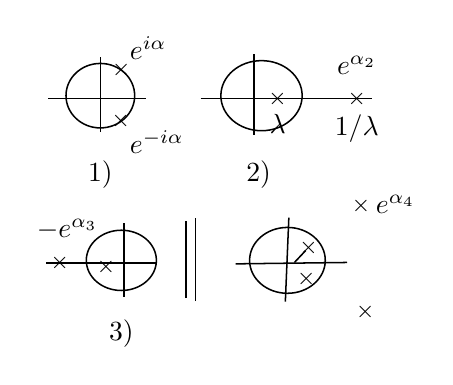
\begin{tikzpicture}[line width=.55pt,scale=.89,
cross/.style={inner sep=0pt,font=\footnotesize}]
\begin{scope}[xshift=.1cm]
\draw (0,0) ellipse[x radius=.49,y radius=.46];
\draw (-.74,-.04)--(.65,-.04) (0,-.52)--(0,.55);
\node[cross] at (.30,.37) {\(\times\)};
\node[cross] at (.29,-.36) {\(\times\)};
\node[above right] at (.28,.37) {\(e^{i\alpha}\)};
\node[below right] at (.28,-.36) {\(e^{-i\alpha}\)};
\node[below] at (0,-.78) {1)};
\end{scope}
\begin{scope}[xshift=2.33cm]
\draw (.07,0) ellipse[x radius=.58,y radius=.50];
\draw (-.80,-.04)--(1.64,-.04) (-.04,-.56)--(-.04,.59);
\node[cross] at (.30,-.04) {\(\times\)};
\node[cross] at (1.43,-.04) {\(\times\)};
\node[below] at (.30,-.13) {\(\lambda\)};
\node[above] at (1.43,.16) {\(e^{\alpha_2}\)};
\node[below] at (1.43,-.13) {\(1/\lambda\)};
\node[below] at (.03,-.78) {2)};
\end{scope}
\begin{scope}[yshift=-2.35cm,xshift=.40cm]
\draw (0,0) ellipse[x radius=.50,y radius=.43];
\draw (-1.07,-.04)--(.49,-.04) (.04,-.52)--(.04,.54);
\node[cross] at (-.88,-.04) {\(\times\)};
\node[cross] at (-.22,-.09) {\(\times\)};
\node[above] at (-.77,.15) {\(-e^{\alpha_3}\)};
\node[below] at (0,-.71) {3)};
\draw (.92,-.54)--(.92,.56) (1.06,-.58)--(1.06,.60);
\end{scope}
\begin{scope}[xshift=2.77cm,yshift=-2.35cm]
\draw (0,0) ellipse[x radius=.54,y radius=.47];
\draw (-.74,-.05)--(.85,-.03) (-.03,-.59)--(.02,.61);
\draw (.10,-.03)--(.26,.14);
\node[cross] at (.30,.18) {\(\times\)};
\node[cross] at (.27,-.26) {\(\times\)};
\node[cross] at (1.05,.77) {\(\times\)};
\node[cross] at (1.11,-.73) {\(\times\)};
\node[right] at (1.12,.80) {\(e^{\alpha_4}\)};
\end{scope}
\end{tikzpicture}}\endgroup\par
Three numbered sketches and an unnumbered fourth. No legible label is visible at the inner cross in the third sketch.}
\end{GelfandAdjacentEvidence}
\begin{GelfandAdjacentEvidence}{GELFAND-P000652}{7}


[At the right of the fourth sketch] --- this only in 3-dimensional space.

\underline{Consider the Fourier coeffs.:}
\[
\varphi_n(a)=\int_0^{2\pi}\varphi(\mu,a)e^{-i\mu n}\,d\mu.
\]
\begin{align*}
1)\quad\varphi_n(a)&=\frac{c}{\sin\dfrac{n\alpha_1}{2}},\\
2)\quad\varphi_n(a)&=\frac{c}{\operatorname{sh}\dfrac{n\alpha_2}{2}},\\
3)\quad\varphi_n(a)&=(-1)^n\frac{c}{\operatorname{sh}\dfrac{n\alpha}{2}}.
\end{align*}
\(c\) depends on the dimension.

[A long enclosing line runs from the three formulas to the entry at right.]

\(1)\quad\alpha_1\) is poorly approx. by rationals (required) \(\Longrightarrow\)
\Unclear{GELFAND-P000652}{approximation-verb}{The word before “approx.” reads “плохо” (poorly).}

\Unclear{GELFAND-P000652}{approximation-parenthesis}{The parenthesis tentatively reads “треб.” (required).}
\end{GelfandAdjacentEvidence}
\begin{GelfandAdjacentEvidence}{GELFAND-P000652}{9}

\[
\text{A)}\quad
\varphi(\mu,a)=\sum_{n=0}^{\infty}
\delta\left(\mu-\left(n+\frac12\right)\alpha-\frac1{2\pi}\right).
\]

(exactly in the reg. sense
\[
\varphi(\mu,a)=\lim_{\varepsilon\to0}\sum_{n=0}^{\infty}
\delta\left(\mu-\left(n+\frac12\right)\alpha e^{-n\varepsilon}-\frac1{2\pi}\right).
\]

[In the lower left margin] \underline{2 quantum numbers} --- 2 indices.

[In the lower left margin] [heavy mark] Infinitely many arithm. progressions.
\Incomplete{GELFAND-P000652}{progression-mark}{Before the line is a heavy mark resembling the letter A.}
\end{GelfandAdjacentEvidence}



\Needspace{7\baselineskip}
\begin{GelfandAdjacentEvidence}{GELFAND-P000653}{1}
\SourcePage{GELFAND-P000653}{unlabelled}
\[
\begin{aligned}
2)\quad\varphi(\mu,a)
&=c\sum_{m,n=-\infty}^{\infty}
\left(
\frac1{\mu-n\cdot2\pi-(m+\frac12)i}
+\frac1{n\cdot2\pi+(m+\frac12)i\,\text{[cancelled mark]}}
\right)\\
&=c\int_0^\mu\wp(\xi)\,d\xi,
\end{aligned}
\]
\(\wp\) --- Weierstrass fn.
\Unclear{GELFAND-P000653}{period-end}{A stroke with several crossbars follows \(i\) in the second denominator. The cancelled letter is undeciphered.}
\end{GelfandAdjacentEvidence}
\begin{GelfandAdjacentEvidence}{GELFAND-P000653}{2}


\SourceFigure{GELFAND-P000653}{pole-lattice}{%
\par\smallskip
\begingroup\color{black}\GelfandFitDiagram{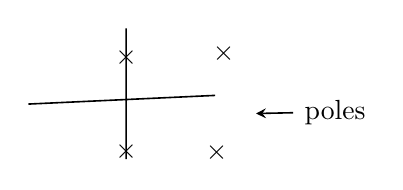
\begin{tikzpicture}[line width=.58pt,>=stealth]
\draw (-1.24,-.08)--(1.13,.03) (0,-.78)--(0,.88);
\foreach \x/\y in {0/.51,1.24/.56,0/-.68,1.15/-.70}
 {\node[inner sep=0pt] at (\x,\y) {\(\times\)};}
\draw[->] (2.12,-.19)--(1.65,-.20);
\node[right] at (2.14,-.19) {poles};
\end{tikzpicture}}\endgroup\par
Crosses on the vertical axis and to its right.}
\end{GelfandAdjacentEvidence}
\begin{GelfandAdjacentEvidence}{GELFAND-P000653}{3}


\SourceFigure{GELFAND-P000653}{curve-figure}{%
\par\smallskip
\begingroup\color{black}\GelfandFitDiagram{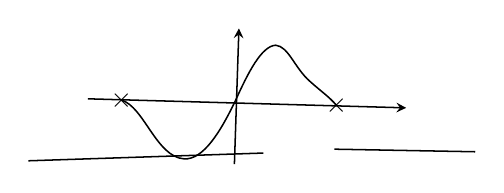
\begin{tikzpicture}[line width=.55pt,>=stealth,x=.82cm,y=.82cm]
\draw[->] (-2.30,.04)--(2.63,-.10);
\draw[->] (-.03,-.97)--(.04,1.13);
\draw (-3.22,-.92)--(.42,-.80) (1.52,-.74)--(3.70,-.78);
\draw (-1.78,.02) .. controls (-1.43,-.08) and (-1.24,-.86) .. (-.81,-.89)
 .. controls (-.51,-.91) and (-.24,-.46) .. (-.01,.02)
 .. controls (.18,.44) and (.39,.86) .. (.61,.87)
 .. controls (.81,.85) and (.90,.52) .. (1.14,.31)
 .. controls (1.33,.14) and (1.44,.07) .. (1.55,-.06);
\node[inner sep=0pt] at (-1.78,.02) {\(\times\)};
\node[inner sep=0pt] at (1.55,-.06) {\(\times\)};
\end{tikzpicture}}\endgroup\par
Curve with a minimum and a maximum, two crosses on the axis, and a broken lower line. A heavy illegible mark lies below the left part of the line.}
\end{GelfandAdjacentEvidence}
\begin{GelfandAdjacentEvidence}{GELFAND-P000653}{4}


Consider the fn.
\[
f(z)=\sum_{k=1}^{\infty}e^{i\lambda_k z}.
\]
Continues analytically downwards with simple poles.

[At right]
\SourceFigure{GELFAND-P000653}{hatched-poles}{%
\par\smallskip
\begingroup\color{black}\GelfandFitDiagram{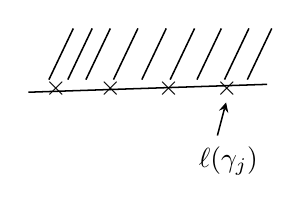
\begin{tikzpicture}[line width=.55pt,>=stealth]
\draw (0,-.02)--(3.03,.08);
\foreach \x in {.26,.50,.73,1.08,1.44,1.80,2.14,2.49,2.78}
 {\draw (\x,.14)--++(.31,.65);}
\foreach \x in {.35,1.04,1.78,2.52}
 {\node[inner sep=0pt] at (\x,.03) {\(\times\)};}
\draw[->] (2.40,-.57)--(2.51,-.15);
\node[below] at (2.54,-.58) {\(\ell(\gamma_j)\)};
\end{tikzpicture}}\endgroup\par
Four crosses on a hatched horizontal line. The arrow from below points to the rightmost cross.}
\end{GelfandAdjacentEvidence}
\begin{GelfandAdjacentEvidence}{GELFAND-P000653}{5}


Fund. sol. of the wave eq. Continuat.

Residues at \(\ell(\gamma_j),\,2\ell(\gamma_j),\,\ldots\) --- Fourier coeffs., etc.
\Unclear{GELFAND-P000653}{pole-order}{The letter with subscript \(j\) in the label and residue line reads \(\gamma\), as in the geodesic notation on the preceding frame.}
\end{GelfandAdjacentEvidence}
\begin{GelfandAdjacentEvidence}{GELFAND-P000653}{6}

\Unclear{GELFAND-P000653}{fourier-overwrite}{The abbreviation before “Fourier” is heavily overwritten and reads “коэфф.” (coeffs.).}
\end{GelfandAdjacentEvidence}



\Needspace{7\baselineskip}
\begin{GelfandAdjacentEvidence}{GELFAND-P000654}{1}
\SourcePage{GELFAND-P000654}{unlabelled}
5/IV-76.\quad \underline{Gelfand Sem.}\quad \underline{Polyakov.}

Action
\[
\left\{\begin{aligned}
S&=\frac1{4e^2}\operatorname{tr}\int A_{\mu\nu}^{2}\,d^4x\\
F_{\mu\nu}&=\partial_\mu A_\nu-\partial_\nu A_\mu+[A_\mu,A_\nu]
\end{aligned}\right.
\]
\Unclear{GELFAND-P000654}{curvature-symbol}{The integrand is written \(A_{\mu\nu}^2\). The next line defines \(F_{\mu\nu}\).}
\end{GelfandAdjacentEvidence}
\begin{GelfandAdjacentEvidence}{GELFAND-P000654}{2}

\(A_\mu^+=-A_\mu\),\quad \(A_\mu\) --- a skew-Herm. matr. \(2\times2\),
which is a fn. on \(\mathbb R^4\).

[Below \(A_\mu\)] \(\mu=0,1,2,3\).

\(A_\mu\) --- the field. \(S\) --- a functional of the field.

Classical eqs. of motion --- stationarity of \(S\).

For numerical \(A_\mu\) --- electromagn. field.

\underline{Analogue for discrete \(x\) and \(t\).}
\[
x=(t,\vec{x}).
\]
\SourceFigure{GELFAND-P000654}{lattice-grid}{%
\par\smallskip
\begingroup\color{black}\GelfandFitDiagram{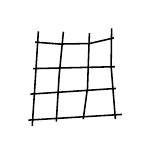
\begin{tikzpicture}[line width=.56pt,scale=.60]
\draw (-.07,0)--(1.91,.12) (-.03,.55)--(1.78,.67)
  (.03,1.09)--(1.76,1.13) (.07,1.65)--(.59,1.61)--(1.22,1.62)--(1.74,1.74);
\draw (.01,-.12)--(.06,.62)--(.14,1.88)
  (.52,-.03)--(.58,.95)--(.67,1.87)
  (1.09,.02)--(1.18,.68)--(1.22,1.84)
  (1.77,.02)--(1.68,1.14)--(1.69,1.94);
\end{tikzpicture}}\endgroup\par
Four roughly horizontal lines and four vertical lines.}
\end{GelfandAdjacentEvidence}
\begin{GelfandAdjacentEvidence}{GELFAND-P000654}{3}

\[
S=\frac{1}{4e_0^2}\sum_{\bar x}\chi\left(
B_{\bar x,\mu} B_{\bar x+\bar a_\mu,\nu}
B^{-1}_{\bar x+\bar a_\nu,\mu} B^{-1}_{\bar x,\nu}
\right).
\]
\Unclear{GELFAND-P000654}{plaquette-notation}{Short bars appear over \(x\) and \(a\) in the product. The bar over the first \(x\) is heavily retraced.}
\end{GelfandAdjacentEvidence}
\begin{GelfandAdjacentEvidence}{GELFAND-P000654}{4}

\(a_\mu\) --- frame,\qquad \(B_{x,\mu}\in SU(2)\).

\(\chi\) --- any character (crossed out)
\Incomplete{GELFAND-P000654}{cancelled-character}{The crossed-out word before “fn.” is illegible.}
\end{GelfandAdjacentEvidence}

(a fn. constant on classes of conj. elements --- e.g. trace).
\[
Z=\int\prod_{\vec x,\mu}dB_{\vec x,\mu}\ e^{-S(B)}.
\]
\(12n\) indep. variables (\(n\) --- the number of lattice sites, at \(\forall\) --- 4 matrices).

\(B_{\vec x,\mu}\) --- indep. vars. \(\Longrightarrow\)
\(dB_{\vec x,\mu}\) --- \underline{inv. measure}
(\(4n\) integrals with inv. measures).
\[
t\to it\quad\Longrightarrow\quad e^{iS}\to e^{-S}.
\]
\underline{In the continuous case --- a functional integral.}

Correl. fns.
\[
\cdots\quad\cdots\quad\cdots\quad\cdots\quad\cdots\quad\cdots
\]


\Needspace{7\baselineskip}
\begin{GelfandAdjacentEvidence}{GELFAND-P000655}{1}
\SourcePage{GELFAND-P000655}{unlabelled}
\underline{12/IV-76.}\quad \underline{Gelfand Sem.}

\underline{\underline{Fuchs.}}\quad \underline{Use of computers in theor. mathematics.}

Comput. of the cohom. of the alg. of formal divergence-free vect. fields

Given \(\mathbb R^n\). consider \((\mathbb R^n)'\) and polynomials
\[
p(\xi_1,\ldots,\xi_q;\eta_1,\ldots,\eta_q),\qquad
\xi_i\in\mathbb R^n,\quad\eta_i\in(\mathbb R^n)'.
\]
They have the property

a) if the pair \(\xi_i,\eta_i\) is put in the place of \(\xi_j,\eta_j\), the polynomial changes sign.

\(dP=P_1\) given by the formula
\begin{align*}
P_1(\xi_1,\ldots,\xi_{q+1},\eta_1,\ldots,\eta_{q+1})
 &=\sum_{i<j}(-1)^{i+j-1}\big[(\xi_i,\eta_j)-(\xi_j,\eta_i)\big]\\
 &\quad P(\xi_i+\xi_j,\xi_1,\ldots,\widehat\xi_i,\ldots,
                \widehat\xi_j,\ldots,\xi_{q+1},\\
 &\qquad\;\;\eta_i+\eta_j,\eta_1,\ldots,\widehat\eta_i,\ldots,
                 \widehat\eta_j,\ldots,\eta_{q+1}).
\end{align*}

\underline{\underline{problem:}} find the cohomology of this complex (still undone).

A computer helped find nontriv. cycles.

Consider those linear in \(\eta\); then this is the cohom. complex of the algebra \(W_n\).

Undone even for \(n=1\).

All results obtained concern this case.

complex \(=\) the sum of many finite-dimensional ones.

Total degree in \(\xi\): \(m_1+q\),
\quad in \(\eta\): \(m_2+q\).
\quad [At right] \(\Vert\) \underline{subcomplex} \(K_{m_1,m_2}\).

(\(q\) varies)

\underline{polys. in \(\xi_1,\ldots,\xi_q,\eta_1,\ldots,\eta_q\).}
\Unclear{GELFAND-P000655}{polynomial-abbreviation}{The first abbreviation tentatively reads “мн-ны” (polynomials).}
\end{GelfandAdjacentEvidence}
\begin{GelfandAdjacentEvidence}{GELFAND-P000655}{2}


Each of them is finite-dimensional.

\(m_1\ne m_2\Longrightarrow\) it is acyclic.

In fact, \(\sum\) homol. of a countable number of subcompls.
\[
H(K)=\bigoplus_m H(K_{m,m}).
\]
(for now \(n\) is arbitrary)

\underline{\(n=1\)}.

\(m=1,2,3\) are acyclic.

\underline{\(m=4\)} nontriv. in dim. \underline{\(7\) and \(10\)}
--- computed on a machine (Gelfand, Fuchs, Kalinin).
\Unclear{GELFAND-P000655}{cohomology-name}{The third surname reads “Калинин” (Kalinin).}
\end{GelfandAdjacentEvidence}
\begin{GelfandAdjacentEvidence}{GELFAND-P000655}{3}


\underline{\(m=5\)} --- “work area overflow \(N=2\)”.

\underline{Euler char.} does not depend on the differential.

\underline{Perchik} (Bott’s grad. student) computed up to \underline{\underline{\(m=35\)}}.
\Unclear{GELFAND-P000655}{perchik-name}{The manuscript spells the surname “Першик”.}
\end{GelfandAdjacentEvidence}
\begin{GelfandAdjacentEvidence}{GELFAND-P000655}{4}

\[
K_{m,m}\supset K'_{m,m}\qquad
H(K_{m,m})=H(K'_{m,m})\otimes H(S^3).
\]
\[
\chi_m^*\text{ --- ?}\qquad(\text{for }K'_{m,m}).
\]
\underline{Perchik found} the generating fn. for \(\chi_m\).
\Unclear{GELFAND-P000655}{series-chi}{After “for” the manuscript has \(\chi_m\) without a star.}
\end{GelfandAdjacentEvidence}
\begin{GelfandAdjacentEvidence}{GELFAND-P000655}{5}


Interesting: prove that for arbitrarily large \(m\) there are \(\chi_m\ne0\).
\Unclear{GELFAND-P000655}{bottom-word-full}{The middle letters are retraced. The word reads “Интересно” (interesting).}
\end{GelfandAdjacentEvidence}

\[
\begin{aligned}
&\tfrac12(1-t^{-1}x^{-1})(1-t^{-1}x)\\
&\qquad (1-x^{-2})\qquad (1-x^2)\\
&(1-tx^{-3})(1-tx^{-1})(1-tx)(1-tx^3)\\
&\ldots
\end{aligned}
\]


\Needspace{7\baselineskip}
\begin{GelfandAdjacentEvidence}{GELFAND-P000656}{1}
\SourcePage{GELFAND-P000656}{unlabelled}
\[
(1-t^\ell x^{-\ell-2})(1-t^2x^{-\ell})\ldots(1-t^\ell x^{\ell+2}).
\]
\Unclear{GELFAND-P000656}{middle-t-power}{The middle exponent of \(t\) is heavily retraced and resembles \(2\). The outer exponents read \(\ell\).}
\end{GelfandAdjacentEvidence}
\begin{GelfandAdjacentEvidence}{GELFAND-P000656}{2}


Take the product of all of them. Discard \underline{everything that contains \(x\)}. Then one obtains
\[
\sum\chi_m t^{2m}=t^{-2}+2-t^8-t^{14}-t^{22}+\ldots+10t^{70}+\ldots
\]
Wrote the expansion through \(t^{70}\).

(Existence proved of \(\geqslant57\) nontriv. [inserted above: classes] of cohomology.)

\underline{\underline{Buchstaber}}\quad \underline{on Adams’s work on Buchstaber’s work.}

\(X\) --- top. space. Consider \(X\times X\to X\) for a group.
\(\Longrightarrow\)

[At left, with arrow to “Consider”] If \(X\) --- an actual group, then,
\[
C(X\times X)\longleftarrow C(X)\quad\text{--- coalgebra struct..}
\]
Roughly:
\[
M(f(x\cdot y))\longleftarrow f(x)
\]
(expected value of the values).

\begin{center}\textemdash\enspace\textperiodcentered\enspace\textemdash\end{center}

\underline{\underline{S. P. Novikov}}\qquad \underline{General theory of relativity.}

\underline{Read:} Landau and Lifshitz (together with Riem. geometry) --- Theory of Fields.

\((t,\vec x)\) --- space of events. \((t,\vec x)\to(x^0,\vec x),\quad x^0=ct\).
\[
\underline{ds^2=g_{ij}\,dx^i\,dx^j},
\qquad
g_{ij}=\begin{pmatrix}
1&&&0\\&-1&&\\&&-1&\\0&&&-1
\end{pmatrix}.
\]
Proper time --- length of a curve.

\underline{Let \(M^4\); given \(g_{ij}\)}.\qquad
\(U\) --- coord. system \(x^0,x^1,x^2,x^3\).
\Unclear{GELFAND-P000656}{coordinate-symbol}{The symbol before “coord. system” tentatively reads \(U\). Its shape resembles Cyrillic И.}
\end{GelfandAdjacentEvidence}
\begin{GelfandAdjacentEvidence}{GELFAND-P000656}{3}


\underline{Einstein:} the metric is called the gravit. field (1913) (+ Grossmann)

\underline{Einstein’s eq.} --- independently Einstein and Hilbert (1916)
\[
\underbrace{R_{ij}-\frac12Rg_{ij}=\frac{8\pi K}{c^4}T_{ij}}.
\]
\Unclear{GELFAND-P000656}{field-equation-k}{The numerator has uppercase \(K\).}
\end{GelfandAdjacentEvidence}
\begin{GelfandAdjacentEvidence}{GELFAND-P000656}{4}


Here \(R_{j\ell}=\sum_i R^i_{ji\ell}\) --- Ricci tensor.

[At right] \(\Vert\) \((R^i_j)_{k\ell}\) --- 2-form
(skew-symm. in \(k,\ell\)) with values in the Lie alg. of the group \(O(n)\).

\(T_{ij}\) --- matter energy-momentum tens. (external mass).

[At right] \(T_{ij}\) accounts for everything except the gravit. field.
\[
R=\sum_{j,\ell}g^{j\ell}R_{j\ell}.
\]
In any dimension
\[
\underbrace{R_{ij}-\frac12Rg_{ij}=T_{ij}}.
\]
Let the phys. quantities be determined by the Lagrangian \(L\).
\[
S=\int L(q,g_{ij})\,\underbrace{\sqrt g\,d^4x}_{d\sigma}.
\]
\(d\sigma\) --- inv. volume elem..

Then
\[
\sqrt g\,T_{ij}=\frac{\delta S}{\delta g_{ij}}.
\]
\Unclear{GELFAND-P000656}{variation-positions}{This fraction has \(g_{ij}\), with lower indices.}
\end{GelfandAdjacentEvidence}


\underline{Electromagn.}
\[
L_{\text{elm.}}=F_{\mu\nu}F^{\mu\nu},\quad
\text{where}\quad F_{\mu\nu}dx^\nu\wedge dx^\mu=d(\vec A).
\]
[Arrow to \(F^{\mu\nu}\)] \underline{the metric enters.}

\underline{No forces:}
\[
\Longrightarrow\quad\frac{\delta S}{\delta g^{ij}}=0,
\qquad S=\int R\sqrt g\,d^4x.
\]


\Needspace{7\baselineskip}
\begin{GelfandAdjacentEvidence}{GELFAND-P000657}{1}
\SourcePage{GELFAND-P000657}{unlabelled}
\underline{Einstein’s eq.:} in the grav. field there is no energy-mom. apart from that in other forms of energy.

\underline{\underline{G.}} Is it quantized? If so, there is no metric (geom. structure of space).

\underline{\underline{N.}} But this affects only \(10^{-33}\) cm
(whereas nuclear interactions at \(10^{-23}\) cm).

As long as space makes sense, Einstein’s eq. holds.

Quantum mech. is limited only by times of \(10^{-43}\) sec.
\[
T_{00}\text{ --- energy density}=\varepsilon>0.
\]
[heading crossed out]
\Incomplete{GELFAND-P000657}{cancelled-heading}{Dense hatching obscures the heading before “Problems”.}
\end{GelfandAdjacentEvidence}
\begin{GelfandAdjacentEvidence}{GELFAND-P000657}{2}

\underline{Problems}

1) \underline{continuum approx.}: hydrodyn. form with Pascal’s law
\[
T_{ij}=(p+\varepsilon)u_i u_j-pg_{ij}.
\]
[At right] (\(p\) --- press., \(\varepsilon\) --- energy density

\(\varepsilon,p,\vec u\) --- fns. of the point.
\[
\varepsilon=\varepsilon(p)\text{ --- given}\qquad\text{or}\quad p=p(\varepsilon).
\]
\underline{Problem:} find \((M^4,g_{ij})\).
Dust-like fluid \(p=0\).

or \(p=\dfrac{\varepsilon}{3}\) --- ultrarelativistic fluid (light

Hydrodyn. --- \(g_{ij}\) --- ordinary metr.
\Unclear{GELFAND-P000657}{hydro-coordinates}{The final abbreviation tentatively reads “метр.” (metric).}
\end{GelfandAdjacentEvidence}
\begin{GelfandAdjacentEvidence}{GELFAND-P000657}{3}

\[
\underline{\sum_k\nabla_k T_i^k=0}\qquad\Longrightarrow\qquad
\text{laws of hydrodyn.}
\]
Field of a point mass
\[
R_{ij}-\tfrac12Rg_{ij}=\delta_{ij}(r,t).
\]
\Unclear{GELFAND-P000657}{stress-index}{The heavily retraced signs on \(\delta\) tentatively read \(ij\).}
\end{GelfandAdjacentEvidence}
\begin{GelfandAdjacentEvidence}{GELFAND-P000657}{4}

symmetry grp. \(SO(3)\) --- \underline{Schwarzschild soln.}.
First \(M^4\) given by Kruskal in 1960.

Spherical coords. describe one chart (and not the whole manifold).

\(r\) in preferred coords. has \underline{saddles} (gravit. radii).

Next time \underline{\underline{Novikov}}.
\Unclear{GELFAND-P000657}{novikov-abbreviation}{The letters before “time” read “След.” (next).}
\end{GelfandAdjacentEvidence}
\begin{GelfandAdjacentEvidence}{GELFAND-P000657}{5}


\underline{19/IV-76.}\qquad \underline{Gelfand Sem.}

\underline{Serre’s problem.} Is every [inserted in a callout: projective]
\(\mathbb C[x_1,\ldots,x_n]\)-module free?
\SourceFigure{GELFAND-P000657}{projective-callout}{%
\par\smallskip
\begingroup\color{black}\GelfandFitDiagram{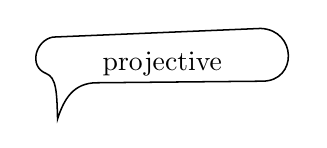
\begin{tikzpicture}[line width=.55pt]
\node at (0,.34) {projective};
\draw (-1.48,.22) .. controls (-1.70,.31) and (-1.61,.64) .. (-1.39,.68)
 -- (1.25,.79) .. controls (1.71,.77) and (1.72,.12) .. (1.27,.12)
 -- (-.83,.10) .. controls (-1.13,.10) and (-1.25,-.11) .. (-1.33,-.36)
 .. controls (-1.34,-.03) and (-1.34,.17) .. (-1.48,.22);
\end{tikzpicture}}\endgroup\par
The word “projective” in an outlined callout before the ring.}
\end{GelfandAdjacentEvidence}
\begin{GelfandAdjacentEvidence}{GELFAND-P000657}{6}


\begin{center}\textemdash\enspace\(\circ\)\enspace\textemdash\end{center}

\underline{Gelfand, following Vaseršteĭn’s notes}
\[
a_1,\ldots,a_k\in\mathbb C[x_1,\ldots,x_n]=A.
\]
is called unimodular if \(\exists p_1,\ldots,p_k:\ \sum p_i a_i=1\).

Is there a matrix with entries in \(A\), and with \underline{\(\det=1\)}
\[
\begin{pmatrix}
a_{11}&\ldots&a_{1k}\\
a_{k1}&\ldots&a_{kk}
\end{pmatrix},
\]
\Unclear{GELFAND-P000657}{matrix-index-corrections}{The indices in \(a_{11},a_{1k},a_{k1}\) are retraced or corrected.}
\end{GelfandAdjacentEvidence}
\begin{GelfandAdjacentEvidence}{GELFAND-P000657}{7}

and with first row [crossed out: \(a_{11},\ldots,a_{1k}\)] \(a_1,\ldots,a_k\)?
\Unclear{GELFAND-P000657}{crossed-first-row}{The indexed row before the corrected first row is crossed out.}
\end{GelfandAdjacentEvidence}


\underline{Drinfeld} on the same topic.

\(B\) --- a ring
\[
f=\begin{pmatrix}f_1\\\vdots\\f_n\end{pmatrix}
\quad\text{--- a unimod. column in }B[x]
\]
(\(x\) --- one var.).

\underline{leading coeff. of \(f_1=1\)}\quad Then \(f(x)\sim f(0)\)
(transformed by a nonsing. matrix over \(B[x]\)).

Main tool --- \underline{resultant}:
\[
\prod(\xi_i-\eta_k)
\]
[At right] \(\xi_i,\eta_k\) --- roots of 2 polys. in 1 var.


\Needspace{7\baselineskip}
\begin{GelfandAdjacentEvidence}{GELFAND-P000658}{1}
\SourcePage{GELFAND-P000658}{unlabelled}
\underline{Main lemma.} Let \(c=\operatorname{Res}(f_1,f_2)\).
Then if \(f\) --- any column, then,
\[
f(Y_1+cY_2)\sim f(Y_1)\quad\text{over }B[Y_1,Y_2].
\]
\Unclear{GELFAND-P000658}{lemma-equivalence}{The relation sign has several retraced wavy strokes. The reading \(\sim\) is tentative.}
\end{GelfandAdjacentEvidence}
\begin{GelfandAdjacentEvidence}{GELFAND-P000658}{2}


\underline{Proof:} by an explicit construction (\underline{Suslin})

\underline{Need:} \(c=1\) and set \(Y_2=-Y_1\).

\underline{Reduction to this lemma.}

A change of var. reduces to the case where \(1\) of the leading coeffs. is \(1\).

Remove all vars. in turn.

\underline{S. P. Novikov.}

\(M^n,g_{ij}\), sign. \((1,-1,-1,-1)\)
\[
R_{ij}-\frac12Rg_{ij}=T_{ij}.
\]
[At right] \(\Vert\) \underline{\underline{Spher. symm. problem}}:
\underline{to completion} \underline{in 1960, Kruskal}.

Phys. formulation of the problem --- hypotheses on \(T_{ij}\).

Continuum
\[
T_{ij}=(p+\varepsilon)u_i u_j-pg_{ij},\quad\text{where }p=p(\varepsilon);
\]
\[
\vec u=(u_0,u_1,u_2,u_3);\qquad 1=\langle u,u\rangle.
\]
Dust: \(p=0\). Speed of sound:
\[
\begin{aligned}
c_{\text{sound}}^2&=\frac{\partial p}{\partial\varepsilon}\geqslant0,\\
c_{\text{sound}}^2&\leqslant c^2=1.
\end{aligned}
\]
There are too few eqs. But there are gauge transfs.

\underline{Hilbert} wrote down the eqs. but gave them up as incorrect.

There is the metric of \underline{Gödel} (that very one) with a closed timelike line (lines?).
\Unclear{GELFAND-P000658}{goedel-line}{The parenthesis reads “линиями?” (lines?) after the singular “линией”.}
\end{GelfandAdjacentEvidence}



\clearpage\section*{Chapter 10}
\Needspace{7\baselineskip}
\begin{GelfandAdjacentEvidence}{GELFAND-P000659}{1}
